\documentclass[a4paper, 11pt]{tubsreprt}
\usepackage[ngerman]{babel}
\usepackage[utf8]{inputenc}
\usepackage{cite}
\usepackage{graphicx}
\usepackage{wrapfig}
\usepackage{subfigure}
\usepackage{hyperref}
\usepackage{blindtext}
\usepackage{amsmath}

\usepackage{ulem}
\title{Gefügeoptimierung einer Fanschaufel aus der Titanlegierung Ti 6Al 4V}
\date{Wintersemester 17/18}
\author{J. Hansen, S. Vodde,
 J. Veer, T. Stein}

\logo{
	
\includegraphics{Bilder/ifw-logo.jpg}
}

\begin{document}
\pagenumbering{roman}
\maketitle
\ \\
\newpage


\chapter*{Eidesstattliche Erklärung}

Wir erklären hiermit an Eides statt, dass wir die vorliegende Projektarbeit ''Gefügeoptimierung einer Fanschaufel aus der Titanlegierung Ti 6Al 4V'' selbstständig verfasst sowie alle
benutzten Quellen und Hilfsmittel vollständig angegeben haben und dass die Arbeit nicht bereits als Prüfungsarbeit vorgelegen hat.\\

\ \\
\ \\
\ \\



Braunschweig, den 26.01.2017


\ \\
\ \\
\ \\
\ \\

(Unterschriften mit Vor- und Zuname) 

\ \\
\newpage
\ \\

\tableofcontents





\chapter*{Einleitung (Steffen Vodde)}
\pagenumbering{arabic}
\addcontentsline{toc}{chapter}{Einleitung}
Titanwerkstoffe gewinnen in der heutigen Zeit zunehmend an Bedeutung. In der Luft- und Raumfahrttechnik sowie der Medizintechnik kann auf die Verwendung von Titanlegierungen nur noch schwer verzichtet werden. Eine geringe Dichte, gute Festigkeitswerte und der Einsatz unter hohen Temperaturen ermöglichen einen vielfältigen Gebrauch dieses Werkstoffes. Insbesondere die Luft-und Raumfahrt profitiert von der Forschung an unterschiedlichen Titanlegierungen. Die Gewichtsersparnis spielt in dieser Thematik eine entscheidende Rolle. Eine Festigkeitssteigerung der verwendeten Titanlegierungen wird angestrebt. Durch diese Steigerung können belastete Bauteile aus Titan geringer dimensioniert werden. Die auftretenden Spannung werden durch einen verringerten Bauteilquerschnitt ertragen und Gewicht wird eingespart. 
  
Im Folgenden befasst sich auch diese Projektarbeit mit der Festigkeitssteigerung einer Titanlegierung. Die Zugfestigkeit der Legierung Ti 6Al 4V soll durch eine Gefügeoptimierung gesteigert werden. Eingesetzt wird diese Legierung in einer Fanschaufel für Flugzeugtriebwerke. Die notwendigen Grundlagen über die Titanlegierung und deren Wärmebehandlung müssen aus geeigneter Literatur erfasst und angewandt werden. Mehrere Gefügezustände sind einzustellen und zu analysieren. Die mechanischen Eigenschafften der einzelnen Gefüge sollen abgeschätzt und erprobt werden. Die erzielten Ergebnisse sollen umfassend beschrieben und ausgewertet werden. Aufbauend auf diese Ergebnisse gilt es diese Zustände zu optimieren.  
 
Die Ausarbeitung befasst sich zunächst mit dem Werkstoff Titan. Anschließend wird insbesondere die Legierung Ti 6Al 4V betrachtet. Der Fokus liegt dabei auf den Gefügemerkmalen, den mechanischen Eigenschaften, sowie den Legierungselementen. Ausgehend von den für die Auswertung notwendigen Methoden und Anwendungen werden die einzelnen Wärmebehandlungen und Strategien dargestellt. Die daraus resultierenden Ergebnisse werden vorgestellt und mit der verwendeten Literatur abgeglichen. Aus den Erklärungen der Festigkeitssteigerung gehen abschließend Schlussfolgerungen hervor.
\newpage
\ \\
\newpage
\chapter{Titanwerkstoffe}\label{Kapitel Titanwerkstoffe}
Dieses Kapitel behandelt die für Titan charakteristischen Eigenschaften. Es wird vorerst auf generelle Eigenschaften eingegangen und dann auf die der Legierung Ti 6Al 4V. Gefügemerkmale, intermetallische Verbindungen und die Eigenschaften der einzelnen Legierungselemente sind Teil dieses Kapitels.
\section{Gefügemerkmale (Tammo Stein)}\label{Abschnitt Gefügemerkmale}
Wie andere Metalle liegt Titan in verschiedenen Gittermodifikationen beziehungsweise Phasenzuständen vor (Allotropie). Der Zustand ist von der Temperatur und den vorliegenden Legierungselementen abhängig. Bei reinem Titan liegt zwischen 1668°C und 882°C ein kubisch raumzentriertes Kristallgitter vor. Diese Phase wird als Beta-Phase ($\beta$-Phase) bezeichnet. Bei 882°C erfährt Titan eine Phasenumwandlung zu einem hexagonalen Gitter. Diese Phasenumwandlungstemperatur wird als Betatransus Temperatur bezeichnet und ist für jede Legierung unterschiedlich, denn die Legierungselemente haben Einfluss auf diese Temperatur \cite{Luetjering2007}.

Das hexagonale Gitter wird als Alpha-Phase ($\alpha$-Phase) bezeichnet. Wenn das Material langsam abgekühlt ist, liegt reines Titan bei Raumtemperatur nahezu vollständig als Alpha-Phase vor. 

Dieses Gitter ist annähernd am dichtesten gepackt. Das Verhältnis in der Zelle ist etwas kleiner, als das in der ideal am dichtesten gepackten Zelle, c/a von Alpha-Titan liegt bei 1.586, wobei c und a die Längen innerhalb einer Zelle sind. Die hexagonal dichteste Packung hat ein Verhältnis von 1.624 \cite{Luetjering2007}. Je nach Aufbau der Zelle sind diese Längen unterschiedlich groß.

Die Phasenumwandlung zwischen Beta- und Alpha-Phase kann auch martensitisch erfolgen. Dabei muss das Material aus einer ausreichend hohen Temperatur abgeschreckt werden. Diese Temperatur wird als Martensitstart Temperatur bezeichnet. Sie ist wie die Betatransus Temperatur von den Legierungselementen abhängig \cite{Luetjering2007}.

\subsection{Alpha-Phase}
Die Alpha-Phase des Titans ist durch eine hexagonale Gitterstruktur gekennzeichnet. Dadurch entsteht ein anisotropes Werkstoffverhalten in einem Korn beziehungsweise Einkristall. In Abbildung \ref{Hexagonale Gitterstruktur} ist das Gitter dargestellt. 

\begin{figure}[h]
\centering
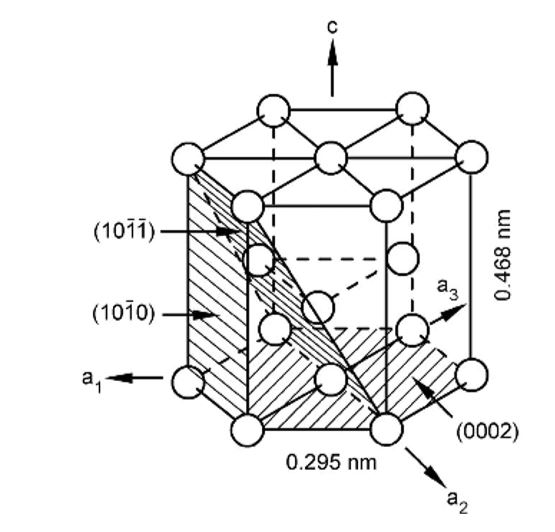
\includegraphics[width=0.5\textwidth]{Bilder/HexagonalesGitter.jpg}
\caption{Hexagonale Gitterstruktur \cite{Luetjering2007}}
\label{Hexagonale Gitterstruktur}
\end{figure}
Ein Einkristall ist über ein homogenes, einheitliches Kristallgitter definiert \cite{Luetjering2007}.
In einem Belastungsfall dieses Einkristalls ist das Werkstoffverhalten abhängig von der Belastungsrichtung im Verhältnis zur Gitterrichtung. Eine Kenngröße, die das elastische Verhalten eines Werkstoffes definiert, ist der Elastizitätsmodul: 
\begin{equation}
E=\sigma*\epsilon.
\end{equation}
Der Elastizitätsmodul ist das Verhältnis zwischen der anliegenden Spannung $\sigma$ und der daraus resultierende Dehnung $\epsilon$.
Es wird in Pascal angegeben. Das Elastizitätsmodul $E$ reicht je nach Verhältnis von minimal 100 GPa bis maximal 145 GPa \cite{Luetjering2007}.

Allerdings wird Titan sehr selten als Einkristall hergestellt, sodass die unterschiedliche Kornorientierung dafür sorgt, dass die Anisotropie der einzelnen Körner sich gegenseitig aufhebt. Somit kann von einem isotropen Werkstoffverhalten ausgegangen werden \cite{Luetjering2007}.


\subsection{Beta-Phase}
Eine Beta-Phase ist ein Gefüge mit einer kubisch raumzentrierten Gitteranordnung. Daraus resultiert ein isotropisches Werkstoffverhalten \cite{Luetjering2007}. Abbildung \ref{Kubischraumzentriertes Gitter} zeigt ein solches Gitter.

\begin{figure}[h]
\centering
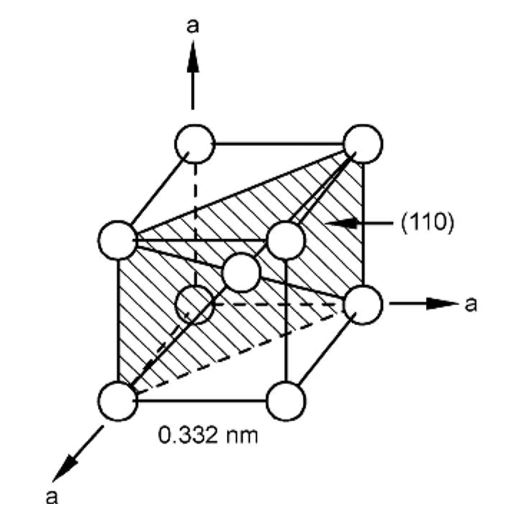
\includegraphics[width=0.5\textwidth]{Bilder/KubischraumzentriertesGitter.jpg}
\caption[Kubisch raumzentriertes Gitter]{Kubisch raumzentriertes Gitter \cite{Luetjering2007}}
\label{Kubischraumzentriertes Gitter}
\end{figure}
Eine große Menge an Beta-Phase existiert in der Regel bei Raumtemperatur nur unter bestimmten Bedingungen. Der aus einem diffusionslosen Umklappvorgang entstehende Martensit wird auch als metastabile Beta-Phase bezeichnet. Durch Zusatz bestimmter Legierungselemente kann die Beta-Phase auch stabil in Raumtemperatur vorliegen. Dies wird im Kapitel  \ref{Kapitel Betastabilisierende Legierungselemente} näher erläutert.
\ \\
Ausgehend von grundlegend verschiedenen Gefügen können diese durch Wärmebehandlung hinsichtlich ihrer mechanischen Eingenschaften optimiert werden. Eine Kombination aus mehreren Gefügeausprägungen können die Vorteile der einzelnen kombinieren. Dazu werden mehrstufige Wärmebehandlungen eingesetzt. Die Proben, die in dieser Arbeit verwendet werden, können nicht mehr rekristallisiert werden, sodass die verbleibenden Wärmebehandlungen auf Parameter wie Korngröße kaum Einfluss nehmen können. Mögliche Gefüge sind also von dem Ausgangsgefüge abhängig.  
\newpage
\subsection{Lamellar} \label{section Gefüge Lamellar}
Rein lamellare Gefüge sind unabhängig von dem Ausgangsgefüge einstellbar. Sie entstehen aus einer langsamen Abkühlung aus dem Beta-Gebiet. Während des Abkühlens bilden sich in den Korngrenzen der Beta-Phase Alpha-Bereiche, die in das Beta-Korn hinein wachsen. Die Alphabereiche wachsen erst in eine Richtung bevor sie ihre Dicke erhöhen. Je nach Abkühlgeschwindigkeit entstehen so dünne oder dickere Bereiche. Die Abbildung \ref{lamellar} zeigt ein beispielhaftes Gefüge, indem voll lamellare Strukturen zu sehen sind \cite{Luetjering2007}.


\begin{figure}
	\centering
		\includegraphics[width=0.5\textwidth]{Bilder/lamellar.jpg}
		\captionof{figure}[lamellares Gefüge]{Volllamellares Gefüge \cite{Leyens2002}}
		\label{lamellar}
		
\end{figure}
\newpage
\subsection{Martensit}
Der Martensit ist eine metastabile Phase, die unter bestimmten Umständen entstehen kann. Aufgrund von Diffusionsvorgängen während eines Glühvorganges verändert sich der Anteil an Legierungselementen innerhalb einer Phase. Dementsprechend reichert sich die Beta-Phase mit Beta stabilisierenden Legierungselementen an. Ist diese Anreicherung zu groß, kann eine martensitische Umwandlung der Beta-Phase nicht statt finden. Um diese Anreicherung zu regulieren, kann die Temperatur verwendet werden. Für eine Martensitbildung muss die Temperatur oberhalb der Martensitstart Temperatur liegen. Bei dieser wird eine zu große Anreicherung vermieden, da die Beta-Phase bei steigendem Volumenanteil eine geringere Konzentration an Beta stabilisierenden Legierungslementen besitzt. Die Martensitstart Temperatur sinkt, je höher die Konzentration an Beta stabilisierenden Elemente in der Phase ist, sodass sie unterhalb der Raumtemperatur liegen kann. Dann ist ein Erzeugen des martensitischen Gefüges nicht mehr möglich.

Neben der Glühtemperatur ist auch die Abkühlgeschwindigkeit entscheidend. Diffusionsvorgänge, die bei einer langsamen Abkühlung stattfinden, finden bei einer martensitischen Umwandlung nicht statt, da Abkühlgeschwindigkeiten von über 500 K/s durch eine Wasserabschreckung vorherschen. Aufgrund der unterschiedlichen Gitterstrukturen der Alpha- und Beta-Phase kommt es so zu einem scherartigen, diffusionslosen Umklappvorgang von einem kubisch raumzentrierten Gitter zu einem hexagonalen Gitter. Anders als bei Stahl kommt es nur zu einer minimalen Gitterverzerrung, da es keine zwangsgelösten Elemente in der Martensit-Phase gibt, die eine Gitterverzerrung verursachen würden. Die entstehende Verzerrung resultiert ausschließlich aus der Umwandlung des Gitters. Das hexagonale Gitter besitzt eine andere Raumausdehnung als das kubisch raumzentrierte Gitter. Durch den Umklappvorgang wandelt sich das Gitter bei konstantem Volumen. Daraus resultiert eine geringe Verzerrung des Gitters \cite{Luetjering2007}. Das charakteristische Martensit-Gefüge wie in Abbildung \ref{vollmartensit} resultiert aus dem Umwandlungsvorgang. Wie bei lamellaren Strukturen entstehen ausgehend von den ehemaligen Korngrenzen des Beta-Korns Nadeln, die in das Korn hinein wachsen. Im Gegensatz zu lamellaren Gefügen sind die Nadeln im Martensit wesentlich feiner \cite{Luetjering2007}.

Liegt eine bestimmte Konzentration an Beta stabilisierenden Elemente vor, verzerren diese metastabil geslösten Elemente das Kristallgitter und es kommt zu einem eher orthorhombischen Gitter. Die ehemalige hexagonale Struktur des Martensits wird auch als $\alpha'$ bezeichnet, das orthorhombrische Gitter als $\alpha''$ \cite{Luetjering2007}. 

\begin{figure}
\centering
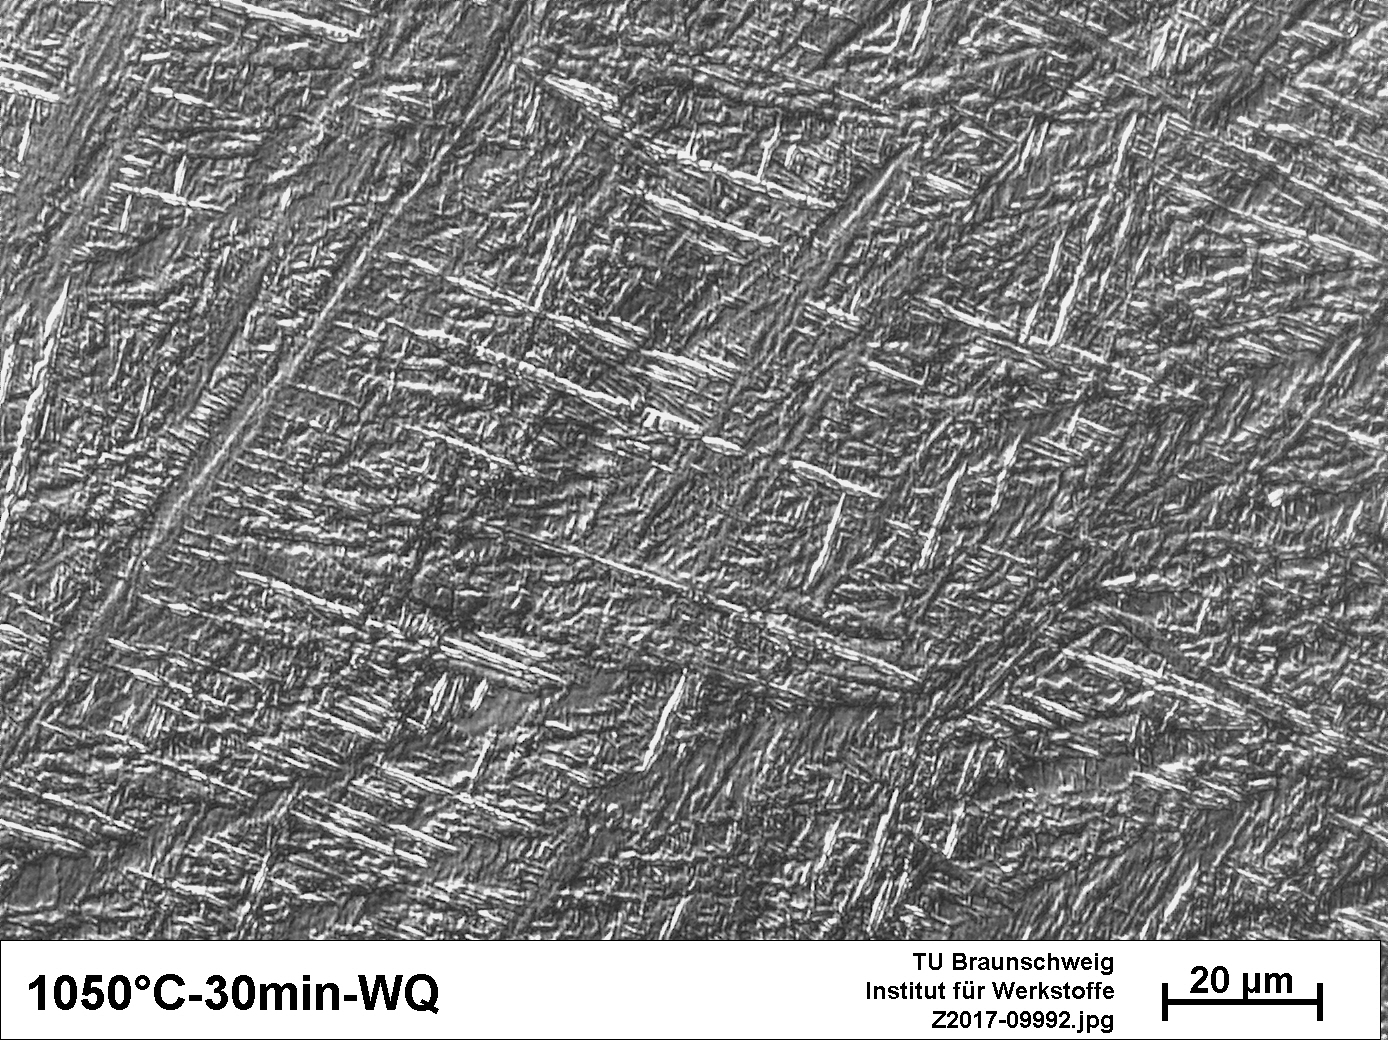
\includegraphics[width=0.4\textwidth]{Bilder/Vollmartensit.jpg}
\caption{Vollmartensitisches Gefüge}
\label{vollmartensit}
\end{figure}
\subsection{Globular}
Die Globulare-Phase besteht aus runden Alpha-Bereichen. Dieses Gefüge resultiert aus einer Rekristallisation. Die Größe der einzelnen Körner ist von der Versetzungsdichte innerhalb des Gefüges vor der Rekristallisation abhängig. Nach einer Rekristallisation ist nur noch eine Zunahme der Korngröße realisierbar. Ausgehend aus diesem Gefüge lassen sich alle relevanten Gefüge einstellen. In Abbildung \ref{globular} erkennt man ein solches Gefüge. 
\begin{figure} %Globulares Gefüge
\subfigure[Globulares Gefüge]{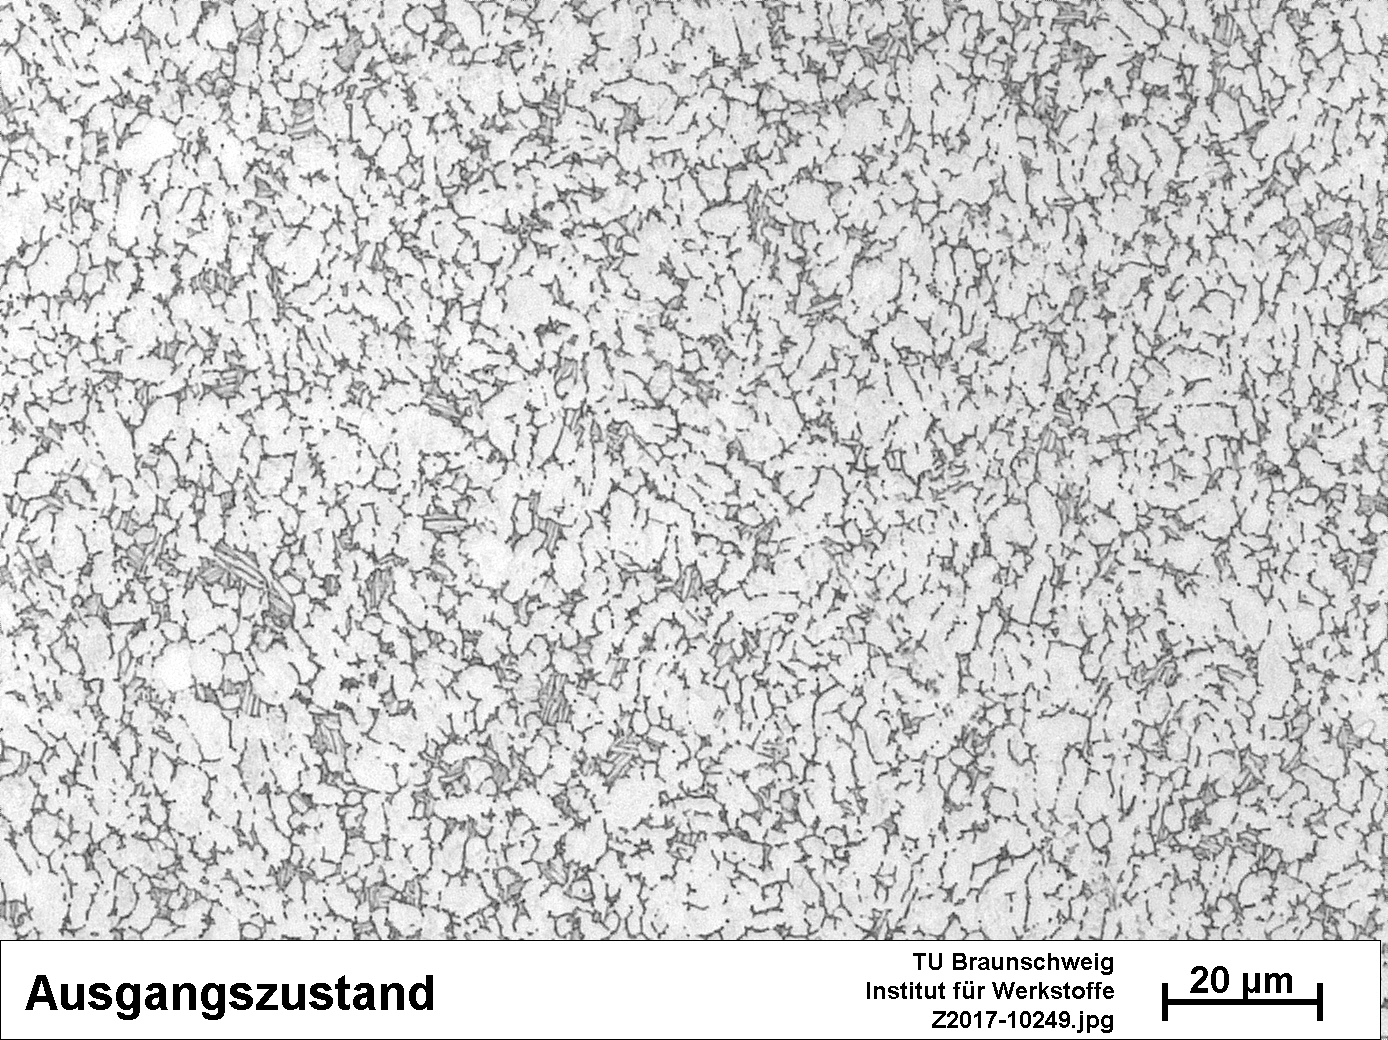
\includegraphics[width=0.5\textwidth]{Bilder/Ausgangsgefuege.jpg}}
\subfigure[Bi-Modal-Gefüge \cite{Werkstoffdesign2012}]{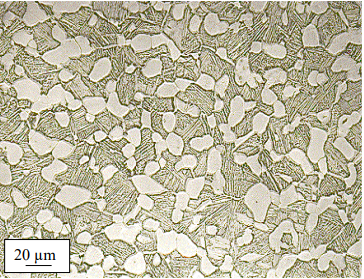
\includegraphics[width=0.5\textwidth]{Bilder/Duplexgefuege.PNG}}
\caption{Globular- und Bi-Modal-Gefüge}
\label{globular}
\label{bimodal}
\end{figure}

\subsection{Bi-Modal}
Bi-Modal-Gefüge (Duplex-Gefüge) sind durch globulare Alpha-Phase und Lamellen aus Alpha- und Beta-Phase gekennzeichnet. In Abbildung \ref{bimodal} ist ein solches Gefüge zu erkennen. 

\newpage
\section{Legierungselemente (Jonas Veer)}
Titanwerkstoffe können durch Zugabe von Legierungselementen in ihren Eigenschaften beeinflusst werden. 
Unterschiedliche Legierungselemente können die Gefügezustände und Umwandlungstemperaturen variieren. 
\subsection{Neutrale Legierungselemente}
\begin{figure}
\subfigure[Einfluss neutraler Elemente auf die Betatransus Temperatur \cite{Luetjering2007}]{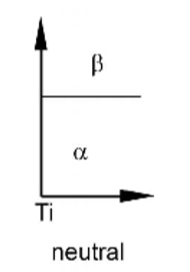
\includegraphics[width=0.3\textwidth]{Bilder/Neutralelegierungselemente.png}}
\subfigure[Titan-Hafnium~ Phasendiagramm \cite{Zwicker1974}]{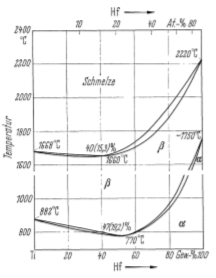
\includegraphics[width=0.3\textwidth]{Bilder/Titanhafniumphasendiagramm.png}}
\caption{Neutrale Legierungselemente}
\label{Abbildung neutrale legierungselemente}
\end{figure}

Zu den neutrale Legierugselementen gehören Zirkonium, Hafnium und Zinn. Sie haben bei niedrigen Konzentrationen keine große Auswirkung auf die Alpha-Beta-Umwandlungstemperatur. Erst bei größeren Konzentrationen zeigt sich ein Einfluss auf die Transformationstemperatur, wie bei Hafnium bei dem die Betatransus Temperatur zunächst ein Minimum durchläuft um bei sehr großen Konzentrationen wieder zu steigen(siehe Abbildungen \ref{Abbildung neutrale legierungselemente}).

\subsection{Alpha stabilisierende Legierungselemente}
\begin{figure}


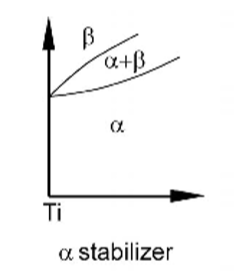
\includegraphics[width=0.25\textwidth]{Bilder/alphastabilisierendelegierungselemente.png}

\caption[Einfluss Alpha stabilisierender Elemente auf die Betatransus Temperatur]{Einfluss Alpha stabilisierender Elemente auf die Betatransus Temperatur \cite{Luetjering2007}}
\label{Alpha stabilisierende Legierungselemente}
\end{figure}
Alpha stabilisierende Legierungselemente zeichnen sich dadurch aus, dass sie die Betatransus Temperatur erhöhen und so die Alpha-Phase bei höheren Temperaturen stabilisieren. Mit steigender Konzentration der Alpha stabilisierenden Elementen steigt die stabilisierende Wirkung und die Betatransus Temperatur erhöht sich weiter (siehe Abbildung \ref{Alpha stabilisierende Legierungselemente}).

Wichtige Vertreter sind hierbei das Substitutionselement Aluminium und die Einlagerungselemente Sauerstoff, Stickstoff und Kohlenstoff.
Um die Alpha stabilisierende Wirkung der Legierungselemente auf die Titanlegierung allgemein auszudrücken wurde das Aluminium-Äquivalent entwickelt (Gleichung \ref{aluminiumequivalent} \cite{Luetjering2007}).
\begin{equation}
[AL]_{eq}=[AL]+0,17[Zr]+0.33[Zn]+10[O].
\label{aluminiumequivalent}
\end{equation}

Es enthält neben Aluminium und Sauerstoff auch die neutralen Elemente Zirkonium und Zinn. Sie haben alleine keinen Einfluss auf die Umwandlungstemperatur, jedoch hat Zirkonium ähnliche chemische Eigenschaften wie Titan und Zinn kann in der intermetallischen Phase Ti$_{3}$Al Aluminium ersetzen.

\subsection{Beta stabilisierende Legierungselemente}\label{Kapitel Betastabilisierende Legierungselemente}

\begin{figure}
\subfigure[Einfluss auf die Betatransus Temperatur]{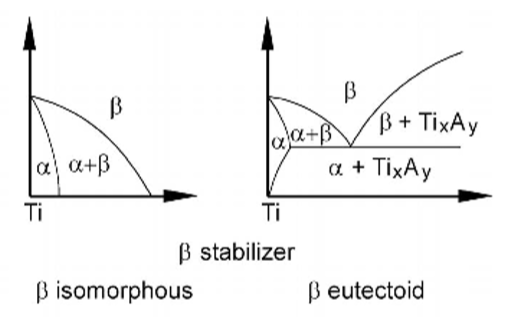
\includegraphics[width=0.5\textwidth]{Bilder/BetastabilisierendeLegierungselemente.png}}
\subfigure[Titan-Vanadium-Phasendiagramm]{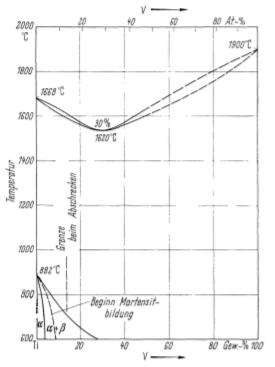
\includegraphics[width=0.35\textwidth]{Bilder/Titanvanadium.png}}
\caption{Beta eutektoide und isomorphe Legierungselemente}
\label{Beta eutektisch isomorphe legierungselemente}
\end{figure}

Durch die Zugabe von Beta stabilisierenden Legierungselementen wird die Betatransus Temperatur von den bei reinem Titan üblichen 882°C gesenkt und erlaubt es bei größerer Konzentration auch bei niedrigen Temperaturen die Beta-Phase zu stabilisieren. Dabei unterteilen sich die Beta-Stabilisatoren in die Gruppen der isomorphen und der eutektoiden Beta-Stabilisatoren.
Wichtige Vertreter der isomorphen Beta-Stabilisatoren sind Vanadium, Molybdän, Niob und Tantal. Durch die Zugabe dieser Elemente ist es möglich die Beta-Phase auf Raumtemperatur zu stabilisieren (siehe Abbildung \ref{Beta eutektisch isomorphe legierungselemente}).
Die Beta-eutektoiden Elemente mit technischer Relevanz sind Eisen, Chrom, und Silizium. Bei Raumtemperatur bilden sie eine Gleichgewichtsphase aus Alpha-Phase und intermetallischen Verbindungen zwischen Titan und dem Legierungselement aus. Das Molybdenequivalent

\begin{equation}
\begin{split}
[Mo]_{eq}=[Mo]+0,2[Ta]+0,28[Nb]+0,4[W]+0,67[V]+1,25[Cr]+ \\
1,25[Ni]+1,7[Mn]+1,7[Co]+2,5[Fe].
\end{split}
\label{Molybdenequivalent}
\end{equation}

beschreibt den quantitativen Einfluss der Beta-Stabilisatoren auf die Legierung \cite{Luetjering2007}.

\subsection{Diffusion von Legierungselementen}\label{Kapitel Diffusion von legierungselementen}
Durch die unterschiedliche Löslichkeit der Legierungselemente in den verschiedenen Kristallgittern der Alpha- beziehungsweise Beta-Phase kommt es im Titan durch Diffusion zum sogenannten ''element partitioning''. Aluminium besitzt eine gute Löslichkeit in der Alpha- wie auch in der Beta-Phase und ist somit eher wenig vom element partioning betroffen.

Da Beta stabilisierende Elemente eine geringe Löslichkeit in der Alpha-Phase besitzen, haben sie die Eigenschaft bei hohen Temperaturen durch Diffusion in die Beta-Phase der Alpha+Beta-Legierung zu fließen. Dies erlaubt weitreichende Wärmebehandlungen, da die Bildung der Ti$_{3}$Al-Phase im Primär-Alpha von der Konzentration von Alpha stabilisierenden Elementen wie auch die Möglichkeit der Martensitbildung von der Konzentration der Beta-Stabilisatoren in der metastabilen Beta-Phase abhängt.
\newpage

\section{Intermetallische Verbindungen (Steffen Vodde)}
Titanlegierungen können, wie alle anderen Metalllegierungen, intermetallische Verbindungen bzw. Phasen bilden. Der Gittertyp der Phase passt meist nicht zu den Gittertypen der einzelnen Komponenten \cite[vgl.]{Domke1986}. Abhängig von den Gittertypen und der Größe der intermetallischen Verbindung können kohärente, teilkohärente oder inkohärente Ausscheidungen entstehen. Die Grenzflächenenergie der kohärenten Teilchen ist gering. Sie verzerren das Kristallgitter nur etwas. Wachsen diese zu inkohärenten Teilchen heran, steigt die Grenzflächenenergie und das Kristallgitter wird stärker verzerrt. 
Bestimmte Titanlegierungen nutzen diese intermetallischen Phasen, um die mechanischen Eigenschaften der Legierung zu verbesseren. Durch eine Ausscheidungshärtung kann die Festigkeit gesteigert werden \cite{Luetjering2007}. Reines Titan kann keine intermetallischen Phasen bilden. Ausschlaggebend hierfür sind die Legierungselemete. Diese Phasen lassen sich in Alpha- und Beta-Phasen aufteilen.  
 

\subsection{Intermetallische Alpha-Phase}
Mit steigendem Aluminium-Äquivalent können sich intermetallische Titan-Aluminium-Phasen bilden, die bei Raumtemperatur beständig sind. Wie das Diagramm \ref{Titan Aluminium Phasendiagramm} zeigt, beginnt dieser Vorgang bereits bei einem Anteil von ca. 5\% Aluminium. Das Zweiphasen-Gebiet $\alpha$Ti und Ti$_{3}$Al bildet sich. Ab einer Temperatur von ca. 500°C können sich Ti$_{3}$Al Teilchen unkontrolliert im $\alpha$Ti ausscheiden. Für die meisten Titanlegierungen gilt jedoch der Richtwert von 6\% Aluminium. Die Ti$_{3}$Al Teilchen besitzen eine hexagonale Gitterstruktur wie das $\alpha$Ti. Die Teilchen können die gleichen Gitterplätze besetzten und verzerren das Kristallgitter nur wenig. Sie sind kohärent. Die Ti$_{3}$Al Teilchen werden vorwiegend für das Ausscheidungshärten genutzt.   

Werden noch größere Anteile Aluminium zum Titan legiert, kann sich TiAl ($\gamma$-TiAl) bilden. Diese Teilchen besitzen ein Tetragonales Kristallgitter. Sie werden in sogenannten Titan-Aluminiden erzeugt. Die Hauptbestandteile dieser Legierungen sind die Phasen Ti$_{3}$Al und TiAl \cite{Luetjering2007}.   
  
\begin{figure}
\centering
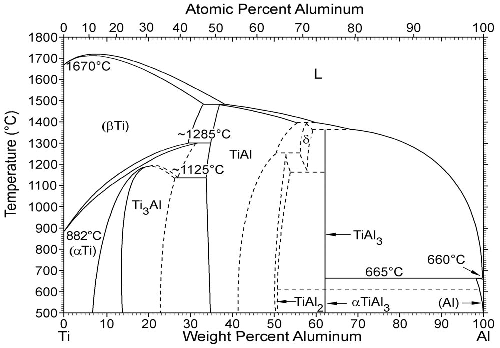
\includegraphics[width=0.5\textwidth]{Bilder/Titanaluminide.png}
\caption[Titan Aluminium Phasendiagramm]{Titan Aluminium Phasendiagram\cite{Luetjering2007}}
\label{Titan Aluminium Phasendiagramm}
\end{figure}

 \newpage
\subsection{Intermetallische Beta-Phasen}
Intermetallische Beta-Phasen sind in Titanlegierungen unerwünscht, da sie meist die mechanischen Eigenschaften verschlechtern. Die isomorphen Stabilisatoren, wie Molybdän, Vanadium oder Niob, bilden in gewöhnlichen Legierungen keine intermetallischen Phasen. Ihre Legierungsanteile sind zu gering. Die eutektoiden Stabilisatoren, wie Chrom oder Eisen hingegen, können schon bei geringen Gehalten intermetallische Phasen bilden. TiFe und Ti$_{2}$Cr Phasen sollen in Titanlegierungen nicht entstehen \cite{Luetjering2007}.   

\section{Ti 6Al 4V (Jannik Hansen)}\label{Kapitel ti64}
Im Mittelpunkt der Aufgabenstellung dieser Arbeit steht der Werkstoff Titan mit den Legierungszusätzen von sechs Gewichtsprozent Aluminium und vier Gewichtsprozent Vanadium (Ti 6Al 4V). Im Folgenden soll demnach ein wenig näher auf die Eigenschaften dieser Legierung eingegangen werden.  
\subsection{Legierungselemente und Verwendung}
Ti 6Al 4V ist die am häufigsten verwendete Titanlegierung weltweit. Sie wurde bereits in den 1950er Jahren entwickelt und zählt zu den am besten erforschten Titanlegierungen \cite{Leyens2002}. Ti 6Al 4V macht etwa 60\% des in Europa und den USA produzierten Titans aus \cite{Sieniawski2013}. Durch seine Legierungselemente Aluminium als Stabilisator der Alpha-Phase und Vanadium als Beta stabilisierendes Element, lässt sich Ti 6Al 4V zu den Alpha + Beta Legierungen zählen. Die genaue Zusammensetzung von Ti 6Al 4V hängt vom Anwendungsbereich und der damit verbundenen Norm ab. Allen gemeinsam liegt aber der Namensgebende Anteil von 6\% Aluminium und 4\% Vanadium zugrunde. Nach DIN EN ISO 5832 sind die in Tabelle \ref{Tabelle Norm Legierungselemente Ti64} aufgeführten Legierungselemente bis zum angegeben Anteil zulässig.

\begin{table}[t]
\begin{tabular}{c|c|c|c|c|c}
Legierungszusatz & Fe & C & N & O & H \\
\hline
Gewichtsprozent nach DIN ISO 5832 & 0.3 & 0.08 & 0,05 & 0,02 & 0,15 \\
\end{tabular}
\caption{Zusätzliche Legierungselemente einer Ti-64 Legierung nach DIN EN ISO 5832}
\label{Tabelle Norm Legierungselemente Ti64}
\end{table}

Die Hauptverwendung der Legierung liegt wie oben bereits erwähnt in der Luftfahrt. Hier kommt sie zum Beispiel als Material für Schaufeln im Fan oder Niederdruckverdichter vor \cite{Luetjering2007}. Weiter findet man Anwendungen in der Medizintechnik. Hier werden gerade Implantate, von denen eine etwas höhere Festigkeit verlangt wird, nicht mehr aus ''commercially pure (CP)'' Titan sondern aus Ti 6Al 4V hergestellt. Das ist insbesondere bei Hüftimplantaten oder Schrauben der Fall \cite{Luetjering2007}.
\subsection{Mechanische Eigenschaften}
\begin{table}
\begin{tabular}{c|c|c|c}
Gefüge & Dehngrenze [MPa] & Zugfestigkeit [MPa] & Bruchdehnung [\%] \\
\hline
bi-modal &	970-170 & 1050-1130 & 10-12 \\
\hline
{$\alpha, \alpha'$} & 800-1100 & 900-1200 & 3-8 \\
\hline
Lamellar & 800-1100 & 900-1200 & 13-16 \\
\hline
Allgemein & 800-1100 & 900-1200 & 13-16 \\

\end{tabular}

\caption[Werkstoffkennwerte für verschiedene Gefüge]{Werkstoffkennwerte für verscheide Gefüge \cite{Chen2008} \cite{Sieniawski2013} \cite{Lee2005}}
\label{Tabelle Spannungen Gefüge}
\end{table}

Die mechanischen Eigenschaften von Ti 6Al 4V hängen wie bei anderen Legierungen des Basiswerkstoffes Titans auch von der abschließenden Wärmebehandlung ab. In Abhängigkeit der durchgeführten Wärmebehandlung schwanken die Angaben in der Literatur. Die Betatransus Temperatur steigt gegenüber der von CP-Titan von ungefähr 882°C \cite[s. 23]{Luetjering2007} und liegt für Ti 6Al 4V zwischen 985°C und 1000°C. Sie wird meist mit 995°C und einer Genauigkeit von 10°C angegeben \cite{Semiatin2003}\cite{Chen2008}. Die Betatransus Temperatur bildet einen zentralen Bezugspunkt für die Einstellung eines Gefüges. Durch seine Legierungselemente ist Ti 6Al 4V in der Lage bei Raumtemperatur sowohl in Alpha- als auch Beta-Phase aufzutreten.
Ein mögliches Gefüge stellt hierbei das Bi-modal- oder Duplexgefüge dar. In Kombination mit einem bis über 200 Stunden andauerndem Auslagern lässt sich hier zusätzlich eine Ausscheidung von Titanaluminiden  herbeiführen. Das Bi-modal-Gefüge in Kombination mit feinsten Ti$_{3}$Al Ausscheidungen verbessert gerade, die schlechten Impact-Eigenschaften von Ti 6Al 4V \cite{Lee2005}. Die schlechten Impact-Eigenschaften sind auf die Bildung adiabater Scherbänder zurück zu führen. Unter hohen Verformungsgeschwindigkeiten kommt es dann in Kombination mit der schlechten Wärmeleitfähigkeit von Titan zu einem schlagartigen Versagen des Werkstoffes.
Ein weiteres mögliches Gefüge stellt das lamellare Gefüge dar. Als lamellare Gefüge versteht man Gefüge, in denen Alpha- und Beta-Phase in feinen Streifen wie in Abschnitt \ref{section Gefüge Lamellar} beschrieben nebeneinander liegen. Die Festigkeit von lamellaren Gefügen hängt maßgeblich von der Größe paralleler lamellarer Bereiche und der Alpha-Lamellenbreite ab. Eine geringe Alpha-Lamellenbreite verspricht hierbei für Ti-64 eine hohe Festigkeit \cite{Sieniawski2013}. Einstellen lassen sich lamellare Gefüge durch ein langsames Abkühlen von oberhalb der Martensit Start-Temperatur. Die Martensit-Start-Temperatur liegt für Ti-64 bei ca. 800°C \cite{Boyer1994}. Ebenfalls sind auch Gefüge möglich, bei denen nur ein Teil als Martensit vorliegt. Ein Beispiel dafür stellt ein Primär Alpha Martensit Gefüge dar. Bei diesem liegt die Alpha-Phase bei Raumtemperatur vor, die Beta-Phase aber hat durch Abschrecken martensitisch umgewandelt. Auch wenn diese nicht mehr zu den lamellaren Gefügen gezählt wird, lassen sich durch diese Gefüge Form erhebliche Festigkeitssteigerungen erzielen. Die Aufgabenstellung dieser Arbeit sieht vor die Zugfestigkeit von Ti 6Al 4V im Hinblick auf eine Verwendung als Triebwerksmaterial zu optimieren. Möglichst hohe Festigkeiten lassen sich dabei mit allen oben aufgezeigten Gefügen erreichen. Einen Überblick gibt Tabelle \ref{Tabelle Spannungen Gefüge}.


\chapter{Angewandte Methodik und Analyseverfahren}

In diesem Kapitel werden die für die Arbeit relevanten Methoden beschrieben und die benötigten Analyseverfahren erläutert.
\section{Wärmebehandlung (Tammo Stein)}

Die Wärmebehandlung nach der Rekristallisation ist die letzte Methode, um das Gefüge des Titans einzustellen. Hierbei kommt es auf Parameter wie Temperatur, Haltezeit und Abkühlmethode an. Um die bereits erwähnten Gefüge zu realisieren, ist eine spezifische Abfolge von einer beziehungsweise mehreren Stufen einer Wärmebehandlung nötig. Die grundlegenden Behandlungen werden in diesem Kapitel behandelt, die speziellen, mehrstufigen, soweit für das Projekt relevanten, im dritten.
\subsection{Temperaturkontrolle}
Für die Temperaturkontrolle innerhalb der Wärmebehandlung kommt ein Ofen zum Einsatz. Dieser kann bis zu Temperaturen deutlich oberhalb der Betatransus Temperatur aufheizen und diese mit einer Genauigkeit von drei Kelvin halten. So kann der Temperaturbereich, der für die Wärmebehandlungen wichtig ist, eingestellt werden. Dieser liegt zwischen Raumtemperatur und 50°C - 100°C oberhalb der Betatransus Temperatur. Der Ofen ist außerdem für die insoweit bedeutende Aufheizgeschwindigkeit verantwortlich.

\subsection{Abkühlmedien}

Durch Abkühlmedien werden bestimmte Abkühlgeschwindigkeiten realisiert. Für langsamere Abkühlungen als in der Luft wird der Ofen genutzt. Hier kann die Temperatur beliebig langsam reduziert werden. Ein weiterer Vorteil des Ofens ist, dass die Probe auf eine bestimmte Temperatur herunter gekühlt werden kann. Dies ist für mehrstufige Wärmebehandlungen wichtig, bei denen eine Abkühlung auf Raumtemperatur zwischen den Schritten vermieden werden soll. 

Da der Ofen nicht überaus schnell abkühlen kann, wird zur schnelleren Abkühlung Luft mit Raumtemperatur verwendet. Durch den höheren Temperaturgradienten im Verhältnis zum Ofen wird so die Abkühlung beschleunigt.  

Um noch schnellere Abkühlungen zu realisieren, wird Wasser oder Öl verwendet. So werden zum Beispiel Abkühlgeschwindigkeiten für eine Martensitbildung ermöglicht.


\section{Anpassung der Gefüge durch Wärmebehandlung (Tammo Stein)}
\begin{figure}
	\centering
	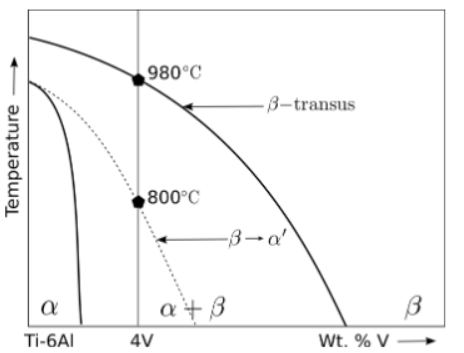
\includegraphics[width=0.5\textwidth]{Bilder/Phasendiagram.PNG}
	\caption[Phasendiagramm]{schematisches Phasendiagramm Ti-6Al-4V \cite{Babu2008}}
	\label{Phasendiagram}
\end{figure}

Das Anpassen der Gefüge ist das Ziel jeder Wärmebehandlung. So werden Werkstoffeigenschaften gezielt für den jeweiligen Anwendungsfall optimiert, denn bestimmte Gefüge, mit bestimmten Mechanische Eigenschaften, folgen aus bestimmten Wärmebehandlungen. Diese Einstellung hat bestimmte Grenzen. Korngrößenreduzierung ist nur durch eine Rekristallisation möglich, sodass im Rahmen dieser Arbeit eine Wärmebehandlung mit Kornwachstum nicht rückgängig gemacht werden kann. Eine derartige Behandlung sollte somit mit bedacht gewählt werden, da gewöhnlich die Festigkeit durch Kornwachstum abnimmt.
\subsection{Lamellar}
Rein lamellare Strukturen folgen aus einer Abkühlung aus dem Beta-Gebiet. In dem Phasendiagramm aus Abbildung \ref{Phasendiagram} ist erkennbar, dass oberhalb der Betatransus Linie das Material in einem Einphasenfeld liegt und somit bei einer moderaten Abkühlgeschwindigkeit vollständig in lamellare Phase umwandelt. Wird die Glühtemperatur unterhalb der Betatransus Temperatur gewählt, ist das Material in einem Zweiphasengebiet. So können unterschiedliche Alphagehalte eingestellt werden, sodass eine Kombination aus Alpha-Phase und Alpha+Beta-Phase entsteht. Die Alphakörner werden auch als Primär Alpha bezeichnet.


Je nach Feinheit der Platten hat das Gefüge positive oder negative Eigenschaften bezüglich der Festigkeit. Fein lamellare Platten sorgen für eine Zunahme der Festigkeit und grobe Platten für eine Abnahme. Dies ist durch die unterschiedliche Grenzflächendichte zu erklären, denn die hohe Anzahl an Körnern behindert den Versetzungsfortschritt. Bei großen lamellaren Platten ist es für die Versetzung deutlich einfacher, durch das Bauteil zu wandern. 
\newpage
\subsection{Martensit}
Martensit entsteht mit Glühtemperaturen höher als die Martensitstart  Temperatur, folgend aus einer Wasserabschreckung. Wie bei lamellaren Gefügen kann auch eine Kombination aus Primärem Alpha und Martensit erfolgen, indem die Glühtemperatur im Zweiphasen-Gebiet gewählt wird. Wie hoch die Temperatur gewählt wird, entscheidet über den Primäralpha-Phasenanteil.

\subsection{Bi-Modal}
Diese Strukturen bestehen aus einer Kombination von Primär-Alpha und lamellaren Strukturen aus Alpha und Beta in den ehemaligen Betakörnern. Dies lässt sich durch eine Wärmebehandlung einstellen, in der die Glühungstemperatur unterhalb der Betatransus-Temperatur liegt. Die Temperatur entscheidet über die Ausprägung der primären Alphakörner. Aus dem Phasendiagramm in Abbildung \ref{Phasendiagram} erklärt sich, dass, je höher die Glühungstemperatur ist, desto geringer ist der primäralpha-Gehalt in dem resultierenden Gefüge. Die Abkühlgeschwindigkeit entscheidet über die Breite der während des Abkühlvorgangs entstehenden Lamellen \cite{Luetjering2007}.

\subsection{Globular}
Wie in Kapitel \ref{Kapitel Titanwerkstoffe} bereits erwähnt, lässt sich ein globulares Gefüge nur durch eine Rekristallisierung ermöglichen. Es ist hierbei wichtig, dass die Glühtempteratur gering und die Haltezeit kurzgehalten werden, um ein Kornwachstum zu verhindern \cite{Luetjering2007}.



\section{Auswertung der Proben}
\subsection{Probenpräparation (Jannik Hansen)}\label{Kapitel Probenpräperation}
Im Folgenden wird auf die Probenpräparation im Anschluss an die Wärmebehandlung im Ofen eingegangen. Ziel der Präparation ist das Erhalten einer geeignete Oberfläche für die Auswertungsverfahren. 

\subsubsection{Trennen}
Um sicher zu gehen, dass bei der präparierten Ebene keine Randeffekte das Ergebnis beeinflussen, wird die Probe mittig getrennt. Das Trennen der Probe geschieht auf einer Trennmaschine vom Modell CUTO 20 der Firma JeanWirtz. Die Schnittebene wird dabei so gewählt, dass die zylindrische Probe senkrecht zur Kreisfläche geteilt wird. Geschnitten wird unter anhaltender Kühlung. Die Kühlung soll eine Veränderung des Gefüges im Bereich der Schnittebene durch zu hohe Temperaturen verhindern. Da die Maschine über keinen automatischen Vorschub verfügt, ist ein gleichmäßiger Vorschub durch einheitliches Kurbeln zu erreichen. Sollten durch den Trennprozess Grate an der Probe entstehen sind diese zu entfernen.
\subsubsection{Einbetten}
Um die Proben später in einer geeigneten Schleif- und Poliermaschine weiter präparieren zu können müssen die Proben auf ein bestimmtes Maß gebracht werden. Das geschieht über das Einbetten der Probe in einen Polymerkörper, welcher anschließend in den Träger der Poliermaschine passt. Zum Einbetten werden grundsätzlich zwei Verfahren verwendet. Beim Warmeinbetten wird ein unter Druck und Temperatur aushärtender Kunststoff verwendet. Beim Kalteinbetten kommt ein Einbettmittel auf Epoxid- oder Acrylbasis zum Einsatz. Diese Einbettmittel bieten den Vorteil der geringen Temperatur beim Aushärten, schmiegen sich aber schlechter an die eigentliche Probe an und haben teilweise eine hohe Aushärtedauer. Da im Rahmen dieser Arbeit keine temperaturempfindlichen Gefügestrukturen wie zum Beispiel Gamma-Titan eingestellt werden sollen, reicht hier ein Warmeinbettverfahren aus. Dabei wird die  Warmeinbettpresse ''SimpliMet 3000'' der Firma Bühler verwendet. Die Probe wird mit der zu betrachtenden Seite nach unten auf den Stempel der Maschine gelegt und mit dem Einbettmedium eingedeckt. Als Einbettmedium wird an der Probe Epomet verwendet, das gut an der Probe haftet. Das Risiko von Lücken zwischen Einbettmedium und Probe wird so minimiert. Ist die Probe bedeckt wird Bakelite verwendet um eine ausreichende Höhe der eingebetteten Probe zu erhalten. Das Einbetten geschieht unter 200 bar Druck und einer Temperatur von 180°C. Die Probe heizt auf, wird zwei Minuten gehalten und wird dann innerhalb von fünf Minuten abgekühlt. Die Abkühlung erfolgt durch das Wasser. 
\subsubsection{Schleifen}
Das Schleifen erfolgt zunächst per Hand auf 240er Schleifpapier um den gesamten Querschnitt der Probe aus dem Einbettmedium freizulegen. Alle Schleifstufen erfolgen nass. Das Wasser dient als Kühl und Schmierstoff und verlängert die Lebensdauer der Schleifkörner gerade auf die Dauer eines Schleifgangs. Das Schleifpapier nach einem Schleifgang ist zu wechseln. Geschliffen wird im Anschluss auf einem Schleifautomat Modell ''Bühler Phoenix 4000''. Dabei wird mit einem Anpressdruck von 8-10N und 150 Umdrehungen pro Minute im Gegenlauf geschliffen. Es erfolgen vier Schleifgänge mit feiner werdender Körnung des Schleifpapieres. Die Schleifgänge erfolgen nach der Tabelle \ref{Tabelle Schleifdauer Körnung}. 
\begin{table}
\begin{tabular}{c|c|c|c|c|c|c}
Körnung & 240 & 320 & 600 & 800 & 1200 & 2500 \\
\hline
Schleifdauer [min] & 0.5 & 1 & 2 & 2.5 & 3 & 3.5 \\
\end{tabular}
\caption{Schleifdauer der einzelnen Schleifstufen}
\label{Tabelle Schleifdauer Körnung}
\end{table}
Nach jedem Schleifgang können sich noch Schleifkörner der vorherigen Körnung auf der Probe befinden. Diese Körner könnten dann im nächsten Schleifgang zu Kratzern auf der Oberfläche führen, welche in der feineren Schleifstufe nicht mehr entfernt werden können. Aus diesem Grund sind die Proben nach jedem Schleifgang für drei Minuten im Ultraschallbad mit Seifenwasser zu reinigen. 

\subsubsection{Polieren}
Im Gegensatz zu einigen anderen Werkstoffen wie zum Beispiel Stahl, kann bei Titan auf Vorpolierstufen verzichtet und direkt mit der Endpolierstufe begonnen werden. Die Endpolierstufe erfolgt in  fünf Minuten Gegen- und anschließender zwei Minuten Gleichlaufpolitur. Poliert wird mit einer OPS Politur und destilliertem Wasser. Die Polierkörner dieser Lösung haben eine mittlere Korngröße von circa 50 nm. Um den Verbleib dieser Körner in ausreichender Zahl auf der Polierscheibe zu sichern, sind jede Minute einige Tropfen der OPS Politur nachzugeben. Nach einem Poliergang sind die Proben drei Minuten in Ethanol im Ultraschallbad zu reinigen. Um Verunreinigungen auf der Probe zu minimieren werden abschließend die Proben mit Ethanol gereinigt und mit einem Heißluftföhn getrocknet.

\subsubsection{Ätzen}
Das Ätzen erfolgt mithilfe eines Ätzmediums nach Kroll (3 ml HF, 6 ml HNO$_{3}$, 100 ml H$_{2}$O). Da die Lösung Flusssäure enthält ist dieser Schritt von geeignetem Personal durchzuführen. Die Probe verbleibt im Falle von Gefügen mit Alpha- und Beta-Phasenanteilen für sechs Sekunden im Ätzmedium und wird anschließend unter Wasser abgewaschen. Bei Proben mit rein martensitischen Gefügen wurde der Verbleib im Ätzmedium auf zehn Sekunden ausgedehnt um bei der späteren Mikroskopie bessere Kontraste zwischen den einzelnen Martensitplatten zu erhalten.

\subsection{Lichtoptische Analyse (Jonas Veer)}

Um herauszufinden, ob die Wärmebehandlung ein Erfolg war, ist der erste Schritt die lichtoptische Analyse der Probenoberfläche am Auflichtmikroskop. Im Labor des IfW steht ein Zeiss Axio Imager 2 zur Verfügung. Das Licht wird aus dem Lichthaus heraus auf einen halbdurchlässigen Spiegel, welcher in einen 45° Winkel befestigt ist, geleuchtet. Von hier aus wird es durch einen Bereich, indem verschiedene Filter eingesetzt werden können, nach unten aus dem auf den Objekttisch reflektiert. Von der Probe wird es zurück in das Objektiv zurückgestrahlt. Hier durchläuft es den halbdurchlässigen Spiegel und wird in das Auge des Betrachters projiziert. 
Zusätzlich verfügt das Mikroskop die Möglichkeit das gesehene Bild mit einer Kamera aufzunehmen und so weitere Bildanalysen durchzuführen. 
Um Martensit in der lichtoptischen Analyse sichtbar zu machen wird ein Polarisationsfilter in das Mikroskop eingesetzt. Dieser Filter polarisiert das Licht linear. Das polarisierte Licht wird auf die Probenoberfläche geführt an welcher es dann reflektiert wird. Hierbei erfährt es einen strukturabhängigen Gangunterschied, welcher sich auf dem Bild als unterschiedliche Graustufen bemerkbar macht.

\subsection{Auszählverfahren (Steffen Vodde)} \label{Kapitel Auszählverfahren}
Das Auszählverfahren ist ein manuelles Hilfsmittel um die Phasenanteile von Gefügen zu ermitteln. Metalllegierungen, wie auch Titan, können unterschiedliche Gefüge mit mehreren Phasen ausbilden. Deren Anteile können mit diesem Verfahren bestimmt werden.

Das zu analysierende Gefüge wird mit einem Mikroskop abgebildet. Fünf zufällig ausgewählte Bildbereiche werden ausgedruckt und mit einem gleichmäßigen Raster versehen. Die Abbildung \ref{Raster für das Auszählverfahren} zeigt ein beispielhaftes Raster.
\begin{figure} %Raster für das Auszählverfahen
\centering
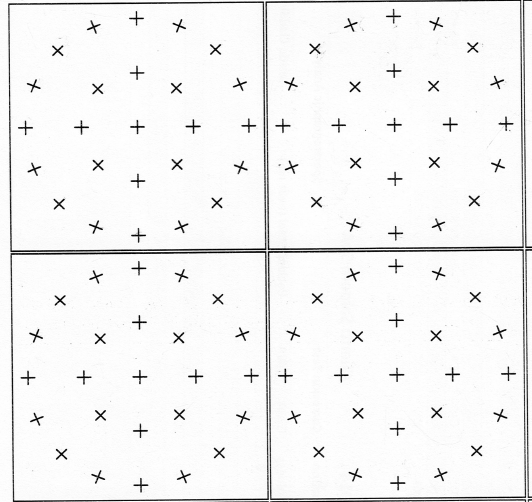
\includegraphics[width=0.3\textwidth]{Bilder/Raster.png}
\caption{Raster für das Auszählverfahren}
\label{Raster für das Auszählverfahren}
\end{figure}

Für eine gleichmäßige Verteilung der Phasen reichen die äußeren Ringe der Felder. Liegen die Anteile allerdings bei wenigen Prozent müssen alle Kreuze berücksichtigt werden. 
Anschließend erfolgt das Auszählen. Die Kreuze die auf der Phase liegen, die bestimmt werden soll, werden mit '1' gezählt. Liegen die Kreuze an einer Phasengrenze, werden sie mit '0,5' gezählt. Berühren die Kreuze die Phase nicht werden sie mit '0' gezählt. Alle Werte werden aufsummiert und durch die Anzahl aller gezählten Kreuze geteilt. Das Ergebnis ist der Phasenanteil. Dieses Verfahren wird an fünf unterschiedlichen Bildbereichen durchgeführt und der Mittelwert gebildet.
\newpage

\subsection{Rasterelektronenmikroskopie (Steffen Vodde)}\label{Kapitel Rasterelektrodenmikroskopie}
Das Rasterelektronenmikroskop (REM) bietet eine bessere Auflösung und eine stärkere Vergrößerung als das Auflichtmikroskop. Es können Vergrößerungen von bis 100000 x erreicht werden. Die Auflösung liegt bei wenigen Nanometern. Durch eingebaute Detektoren am REM können bestimmte analytische Methoden zusätzlich durchgeführt werden. Eine genauere Gefügebeurteilung ist dadurch möglich.  

Die Funktionsweise wird im Folgenden kurz erläutert. Ein Wolframdraht oder ein Lanthanhexaborideinkristall (LaB$_{6}$) dient als Elektronenquelle. Die Elektronen werden emittiert und mittels Beschleunigungsspannung in Richtung Anode abgelenkt. Je nach Auflösung kann die Spannung zwischen 200V und 50kV variieren. Elektromagnetische Linsen bündeln die Elektronen in einem Strahl und lenken ihn auf die Probe. Mit einer Anblenkspule kann der Strahl über die Probe geführt werden (siehe Abbildung \ref{REM Aufbau}).  


\begin{figure} %REM Aufbau
\centering
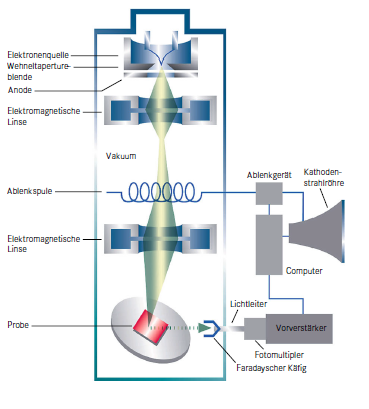
\includegraphics[width=0.5\textwidth]{Bilder/REM.png}
\caption[Aufbau eines Rasterelektronenmikroskops]{Aufbau eines Rasterelektronenmikroskops \cite{Welsch2015}}
\label{REM Aufbau}
\end{figure}


Die Elektronen gelangen auf die Probeoberfläche und es entstehen Wechselwirkungen zwischen den Strahlelektronen und den Atomen der Probenoberfläche. Die zwei wichtigsten Erscheinungen sind hierbei die Rückstreuelektronen (RE) und die Sekundärelektronen (SE). Die Strahlelektronen werden durch die Atomkerne in der Probe abgelenkt und verlieren an Energie. Diese Energie wird in Form der Röntgenbremsstrahlung frei. Die dabei teilweise zurückgeworfenen Elektronen werden als RE bezeichnet. Der Streuprozess zwischen den Strahlelektronen und den Elektronen in den Atomschalen führt zu SE. Die entstandene Röntgenstrahlung, ist die charakteristische Röntgenstrahlung. Die Elektronen in den Atomschalen werden von den Strahlelektronen herausgeworfen. Die Schale ist ionisiert. Diese freien Plätze werden durch andere Elektronen besetzt. Die dabei frei werdende Energie wird in Form von Röntgenstrahlung emittiert. Verlassen RE die Probe können zusätzlich SE entstehen.

Die SE und RE dienen nun der Bilderzeugung. Die Elektronen werden mit jeweils unterschiedlichen Detektoren erfasst. Die Spannung, die aus dem Detektorimpuls erzeugt wird, gelangt zur Kathodenstrahlröhre. Werden viele Elektronen erfasst, steigt die Spannung und der Bildpunkt erscheint hell. Die einzelnen Bildpunkte werden nun durch das ''abrastern'' der Oberfläche erzeugt. Heutzutage erfolgt die Bildherstellung digital\cite{Welsch2015}.

Gute Bildergebnisse können nur durch eine sorgfältige Probepräparation entstehen. Die Oberflächen müssen sauber sein. Die Proben sollten vor der Analyse im Ultraschallbad gereinigt werden.  Zudem muss die gesamte Probe elektrisch leiten. Eingebettete Proben können nicht verwendet werden. Der Kunststoff nimmt die Elektronen auf und würde den Elektronenstrahl ablenken. Alternativ kann eine leitende Gold oder Silberschicht aufgebracht werden.   

\subsection{Energiedisperive Röntgenspektroskopie (Steffen Vodde)}\label{Kapitel EDX}

Die Energiedisperive Röntgenspektroskopie (EDX) wird vor allem in der Werkstoff- und Materialtechnik eingesetzt. Die EDX ermöglicht die Elementverteilung in der Oberfläche von unterschiedlichen Materialien  darzustellen. Die Elementverteilung in bestimmten Gefügebereichen kann so visualisiert werden (z.B. element partitioning).
Wird ein Elektronenstrahl auf eine Probenoberfläche beschleunigt (siehe Kapitel \ref{Kapitel Rasterelektrodenmikroskopie}), entsteht die charakteristische Röntgenstrahlung. Je nach Element besitzt diese Strahlung eine bestimmte Energie. Die Formel

\begin{equation}
E_{ n }=\frac{ 1 }{ n^{ 2 } }*\frac{ m_{ 0 } }{ 8 }*\left( \frac{ Z*e^{ 2 } }{ \epsilon_{ 0 }*h } \right)^{ 2 }
\end{equation}
(E$_{n}$: Energie, n: ganze Zahl, m$_{0}$: Elektronenmasse, Z: Ordnungszahl, e: Elementarladung, $\epsilon_{0}$: Influenzkonstante, h: Plancksches Wirkungsquantum)\cite{Gemming2013}

zeigt, dass die Energie von der Ordnungszahl des Elements abhängig ist. Diese Energie wird in eine charakteristische Wellenlänge umgewandelt. Nach der Formel  

\begin{equation}
\lambda_{ min }=\frac{ h*c }{ E_{ 0 } }
\end{equation}
(c: Lichtgeschwindigkeit, $\lambda$: Wellenlänge)\cite{Gemming2013}

ist das Verhältnis zwischen der Energie und Wellenlänge antiproportional.

\newpage
Die charakteristischen Röntgenstrahlen werden auf einen Halbleiterkristall gelenkt. Dieser wandelt die Energie der Strahlung in eine Spannung um. Diese Spannung wird aufgezeichnet und im Röntgenspektrum als Peak dargestellt. Je höher der Elementanteil, desto höher ist die Intensität des Peaks. Die Summe aller Ausschläge ergibt 100\%. Die Intensität aller Peaks ist abhängig von der Zeit, in der Elektronenstrahl auf die Probenoberfläche trifft. 
Jedes Element besitzt meist mehrere Elektronenschalen, die angeregt werden können. Werden diese Schalen ionisiert, emittieren sie Röntgenstrahlung mit unterschiedlicher Wellenlänge. Je nach Element können so mehrere Peaks mit einer spezifischen Röntgenenergie im Spektrum entstehen (siehe Abbildung \ref{Röntgenspektrum1}). Je nach angeregter Schale (L oder K) entstehen Peaks für das Zirconium. Die Ausschläge im Bereich niedriger Wellenlänge sind auf die Bremsstrahlung der einzelnen Elemente zurückzuführen. Zudem kann es vorkommen, dass sich einzelne Peaks von unterschiedlichen Elementen überlagern. Dies erschwert die Zuordnung der einzelnen Ausschläge \cite{Gemming2013}. 

\begin{figure}
\centering
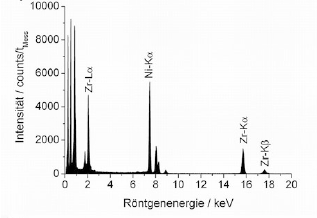
\includegraphics[width=0.66\textwidth]{Bilder/Roentgenspektrum.png}
\caption[Röntgenspektrum]{Röntgenspektrum \cite{Gemming2013}}
\label{Röntgenspektrum1}
\end{figure}

Jeder Ausschlag im Röntgenspektrum muss eindeutig zugeordnet werden, um eine qualitative Aussage über die Elementverteilung abzugeben. Um eine Zuordnung vorzunehmen, müssen die einzelnen Wellenlängen bzw. Röntgenenergien der Elemente bekannt sein. Für ein aussagekräftiges Röntgenspektrum sollte die Strahlzeit des Elektronstrahls großzügig gewählt werden.   

\newpage


\subsection{Härteprüfverfahren nach Vickers (DIN EN ISO 6507-1) (Jannik Hansen)} \label{Kapitel Härte}
Die im Rahmen dieser Arbeit durchgeführten Härteprüfungen erfolgen alle nach dem Verfahren nach Vickers. Das Verfahren nach Vickers eignet sich besonders für Laborprüfungen, da mit ihm sowohl niedrige als auch hohe Härten ermittelt werden können. Um den Härtewert einer Probe zu ermitteln wird ein LECO LV 100AT verwendet. Der Härtewert einer Probe wird durch die Auswertung von fünf Eindrücken ermittelt. Die Eindrücke werden dabei auf einer Geraden gleichmäßig auf der Probe verteilt. Dabei ist darauf zu achten ausreichend Abstand zum Rand zu lassen, damit Randeinflüsse vermieden werden. Der Abstand von Rand und zwischen den Eindrücken ist genormt.
Erzeugt werden die Eindrücke unter einer Prüfkraft von 10 Kilopond was etwa 98,1 Newton entspricht. Die Prüfdauer beträgt nach Norm 15 Sekunden. An den ermittelten Härtewert wird die Prüfkraft HV10 angehängt. Der Härtewert ergibt sich als Quotient der aufgebrachten Prüfkraft $F$ und dem Mittelwert der Diagonalen $d$ des quadratischen Prüfeindrucks nach Formel \ref{Vickershärte formel}.

\begin{equation}
HV = \frac{ 0.102 F * 1.8544 }{ d^{ 2 } }.
\label{Vickershärte formel}
\end{equation}


Durch die verwendete Prüfapparatur, das verwendete Messverfahren nach Vickers und die aufgebrachte Prüfkraft, kann von einer Ungenauigkeit der ermittelten Härtewerte von 3\% ausgegangen werden.
Nach der Quelle \cite{Donachie2001} existiert zwischen Härtewert und Zugfestigkeit bei Titanwerkstoffen lediglich eine sehr schlechte Korrelation. Trotzdem lässt die Ermittlung des Härtewertes eine Abschätzung auf die Zugfestigkeit zu. Um eine endgültige Aussage über die Festigkeit des Titans nach der Wärmebehandlung treffen zu können, ist ein Zugversuch durchzuführen.


Exemplarisch für die Bestimmung der Zugfestigkeit aus der Vickershärte, seien im Folgenden zwei Möglichkeiten aufgezeigt. Eine Diskussion dieser Formeln und der nach Quelle \cite{Donachie2001} schlechten Korrelation von Zugfestigkeit und Härte in Titan wird an spätere Stelle stattfinden.
Nach Ulrich Zwickert gilt für die Zugfestigkeit  $\sigma_{B}$  folgende Gleichung:

\begin{equation}
\sigma_{B}=\alpha*HV.
\label{Zugfestigkeit}
\end{equation}

Der Vorfaktor $\alpha$ wird hierbei zwischen 0,31 und 0,35 angegeben. Die Spannung $\sigma_{B}$ wird in diesem Fall in $kp/mm^{2}$ angegeben. Für eine Umrechnung in MPa muss mit 9,81 multipiziert werden. Wichtig ist auch, dass Zwickert von Härtewerten HV30 ausgeht. Ebenfalls soll die Gleichung nur bei Zugfestigkeiten von 882 MPa bis 1226 MPa gelten \cite{Zwicker1974}. Da die Vickershärte oberhalb einer Prüfkraft von 5,1 $kp$ unabhängig von der aufgebrachten Prüfkraft wird, sollten die hier ermittelten Härtewerte HV10 nur minimale Abweichungen zu den Härtewerten HV30 liefern. 
Quelle \cite{Shi2013} gibt nach folgender Gleichung einen möglichen Zusammenhang zwischen Dehngrenze $\sigma_{0,2}$ und Vickershärte HV:
\begin{equation}
\sigma_{0,2} = 3,013 HV - 127,012.
\label{Formel zusammenhang dehngrenze vickershärte}
\end{equation}

Weiter soll der Zusammenhang zwischen Dehngrenze und Zugfestigkeit wie folgt dargestellt werden können: 
\begin{equation}
\sigma_{B} = 1,1907\sigma_{0,2} - 86,63.
\label{Formel zusammenhang dehngrenze und Zugfestigkeit}
\end{equation}

Die Autoren beziehen sich in ihrer Arbeit jedoch auf elektronenstrahlgeschweißte Wertstücke \cite{Shi2013}.
\subsection{Zugversuch (DIN EN ISO 6892-1 Teil B) (Tammo Stein)}
\label{Kapitel Zugversuch}
Bei einem Zugversuch werden Proben bis zum Bruch gedehnt und dabei Werkstoffkennwerte bestimmt. Die Kennwerte sind unter anderem  Elastizitätsmodul, Elastizitätsgrenze, Zugfestigkeit und Bruchdehnung. Unter diesen Kennwerten ist für die Anforderung der Arbeit die Zugfestigkeit interessant, da diese über eine Wärmebehandlung optimiert werden soll. Sie ist die größte zu ertragene Spannung bevor sich das Bauteil einschnürt beziehungsweise reißt. Der Zugversuch wird mit einer Universalprüfmaschine der Firma Zwick Roell nach der Norm DIN EN ISO 6892-1 Teil B durchgeführt. Dabei werden die Zugproben nach DIN 50125-B5x25 angefertigt. Nach der Norm des Zugversuches wird die Spannungsgeschwindigkeit abhängig von dem Elastizitätsmodul des Werkstoffs gewählt. Da Titan ein E-Modul kleiner 150000 $MPa$ besitzt, wird eine Spannungsgeschwindigkeit zwischen 2 und 20 $MPa$~ $s^{-1}$ gewählt. Diese Spannungsgeschwindigkeit wird während der Bestimmung der Dehngrenze verwendet. Danach wird eine Dehngeschwindigkeit von maximal $0,008$ $s^{-1}$ zur weiteren Messung gewählt. Form B der Zugproben sind nach Norm Rundproben mit Gewinde. Der Zusatz ''5x25'' beschreibt die Maße der Probe. Fünf Millimeter im Probendurchmesser und 25 Millimeter in der Anfangsmesslänge.



\chapter{Wärmebehandlungsstrategien}
Die vorliegende Titanlegierung Ti 6Al 4V besitzt ein globulares Ausgangsgefüge, bestehend aus Alpha- und transformierter Beta-Phase (siehe Abbildung \ref{ausgangsgefüge Kapitel3}). Die Härte im Ausgangszustand beträgt circa 305 HV10. Ausgehend von diesem Zustand soll die statische Festigkeit gesteigert werden. Der Härtewert dient hierfür als erster Richtwert (siehe Kapitel \ref{Kapitel Härte}). Die gegebenen Proben werden unterschiedlichen Wärmebehandlungen unterzogen und metallografisch ausgewertet. 

\begin{figure}[h]
\centering
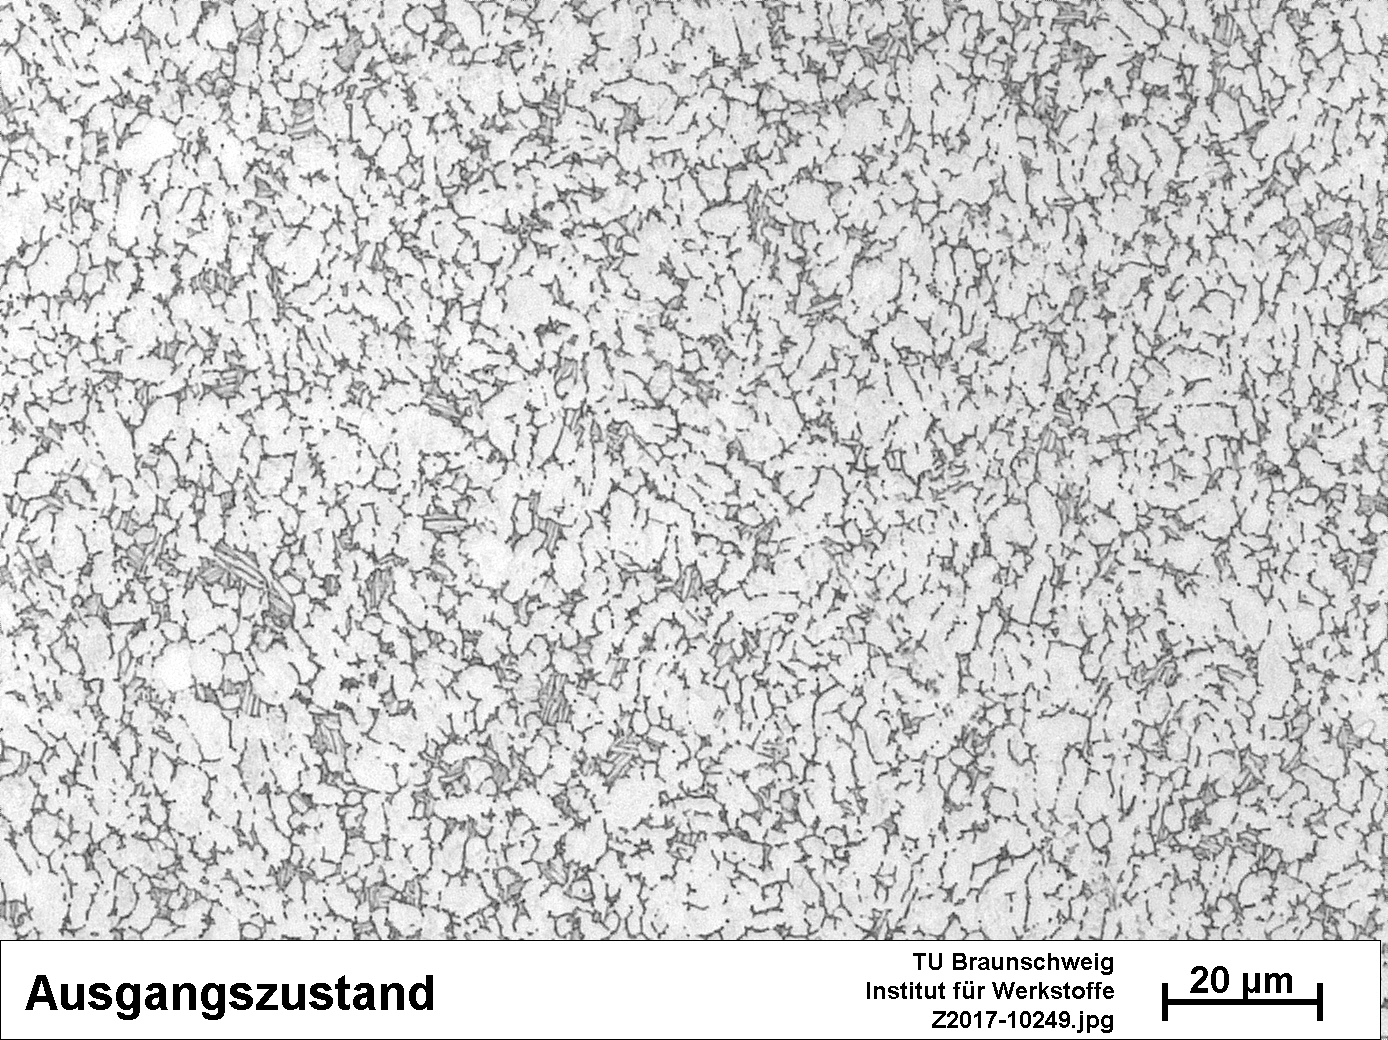
\includegraphics[width=0.7\textwidth]{Bilder/Ausgangsgefuege.jpg}
\caption{Ausgangsgefüge, Alpha- und transformierte Beta-Phase}
\label{ausgangsgefüge Kapitel3}
\end{figure}

\newpage
\section{Festigkeitssteigerung durch Primär-Alpha-Martensit-Gefüge (Steffen Vodde)}\label{Festigkeitssteigerung durch Martensitbildung}
Die Literaturrecherchen zeigen, dass sich die mechanischen Eigenschaften der Titanlegierung durch unterschiedliche Gefügestrukturen beeinflussen lassen. Das erste angestrebte Gefüge besteht aus primär Alpha ($\alpha$) und Martensit ($\alpha'$). Ausgehend von diesem Gefüge beeinflusst eine anschließende Alterung die mechanischen Eigenschaften. Ein  Verhältnis aus hoher Festigkeit und guter Duktilität kann so eingestellt werden \cite{Gilbert1990}. Der erste Schritt dieser zweistufigen Wärmebehandlung ist das Einstellen eines Gefüges aus primärer Alpha- und Martensit-Phase.
 
Einen großen Einfluss auf die mechanischen Eigenschaften hat hierbei die Alpha-Phase. Der Volumenanteil und die Größe der Alpha-Körner beeinflussen diese Eigenschaften und die Verteilung der Legierungselemente, die damit Auswirkungen auf die spätere Alterung des Gefüges haben. Der Anteil ist dabei abhängig von der gewählten Glühtemperatur. In der Quelle \cite{Sahoo2015} wird die Variation der Alpha-Phase in einem Bi-Modal-Gefüge durch unterschiedliche Glühtemperaturen dargestellt. Mit abnehmendem Alpha-Anteil wird die Härte gesteigert und die Elementverteilung gesteuert. Die hier angewandte Methodik wird auf das gewünschte Martensit-Gefüge übertragen.
Mit einer Wärmebehandlung im Zweiphasengebiet (Alpha + Beta) und anschließendem Wasserabschrecken der Proben, wird das gewünschte Gefüge erzeugt. Bei steigender Glühtemperatur sinkt der Anteil der Alpha-Phase bis die Betatransus Temperatur erreicht und keine Alpha Phase mehr vorhanden ist (siehe Abbildung \ref{Phasendiagram}).  Durch das Abschrecken wird dieser Zustand eingefroren und die Beta-Phase wandelt diffusionslos in den Martensit um. Drei Proben werden bei unterschiedlichen Glühtemperaturen knapp unterhalb Betatransus geglüht und anschließend abgeschreckt.

\newpage
\subsection{Abhängigkeit des Primär-Alpha-Anteils von der Glühtemperatur}
Der Alpha-Anteil wird durch die unterschiedlichen Glühtemperaturen im Zweiphasen Gebiet eingestellt. Dazu wurden drei Proben bei jeweils 950°C, 960°C und 970°C für eine Stunde im Ofen geglüht und anschließend im Wasser abgeschreckt. Nach der Probenpräparation (siehe Kapitel \ref{Kapitel Probenpräperation}) folgt die metallografische Untersuchung. Die Abbildung \ref{Alle Glühen} zeigt die lichtmikroskopischen Aufnahmen. Die durchgeführte Wärmebehandlung erzeugt das gewünschte Gefüge. Primär Alpha-Körner liegen in einer Matrix aus Martensit. Die Alpha-Körner wurden durch das Abschrecken eingefroren. Die Beta-Phase ist komplett in den Martensit umgeklappt. In den Abbildungen sind die unterschiedlichen Alpha-Anteile klar zu erkennen. Mit steigender Glühtemperatur nimmt, wie erwartet, der Anteil ab. 

Die genauen Phasenanteile sind mittels Auszählverfahren (siehe Kapitel \ref{Kapitel Auszählverfahren}) bestimmt worden. Aus der Tabelle \ref{Härte in Abhängigkeit der Glühtemperatur} wird ersichtlich, dass bei einer Glühtemperatur von 950°C circa 20\% Alpha-Phase vorliegt. Dieser Anteil sinkt auf circa 6\% bei einer Temperatur von 970°C. Unter dem Auflichtmikroskop sind diese geringen Anteile nur noch schwer zu erkennen.  
\begin{table}[h]	%Härte in Abhängigkeit der Glühtemperatur
\begin{tabular}{c|c|c|c}
Wärmebehandlung	& Primär Alpha Anteil [\%] &	Mittelwert 
Härte in HV10 	& Standardabweichung \\
\hline
950°C 1h WQ	& 	20	&	343	&	6,68 \\
960°C 1h WQ	&	13	&	351	&	9,07 \\
970°C 1h WQ	&	6	&	357	&	8,95 \\

\end{tabular}
\caption{Härte in Abhängigkeit der Glühtemperatur}
\label{Härte in Abhängigkeit der Glühtemperatur}
\end{table}

\begin{figure}
\subfigure[Gefüge bei einer Glühungstemperatur von 970°C]{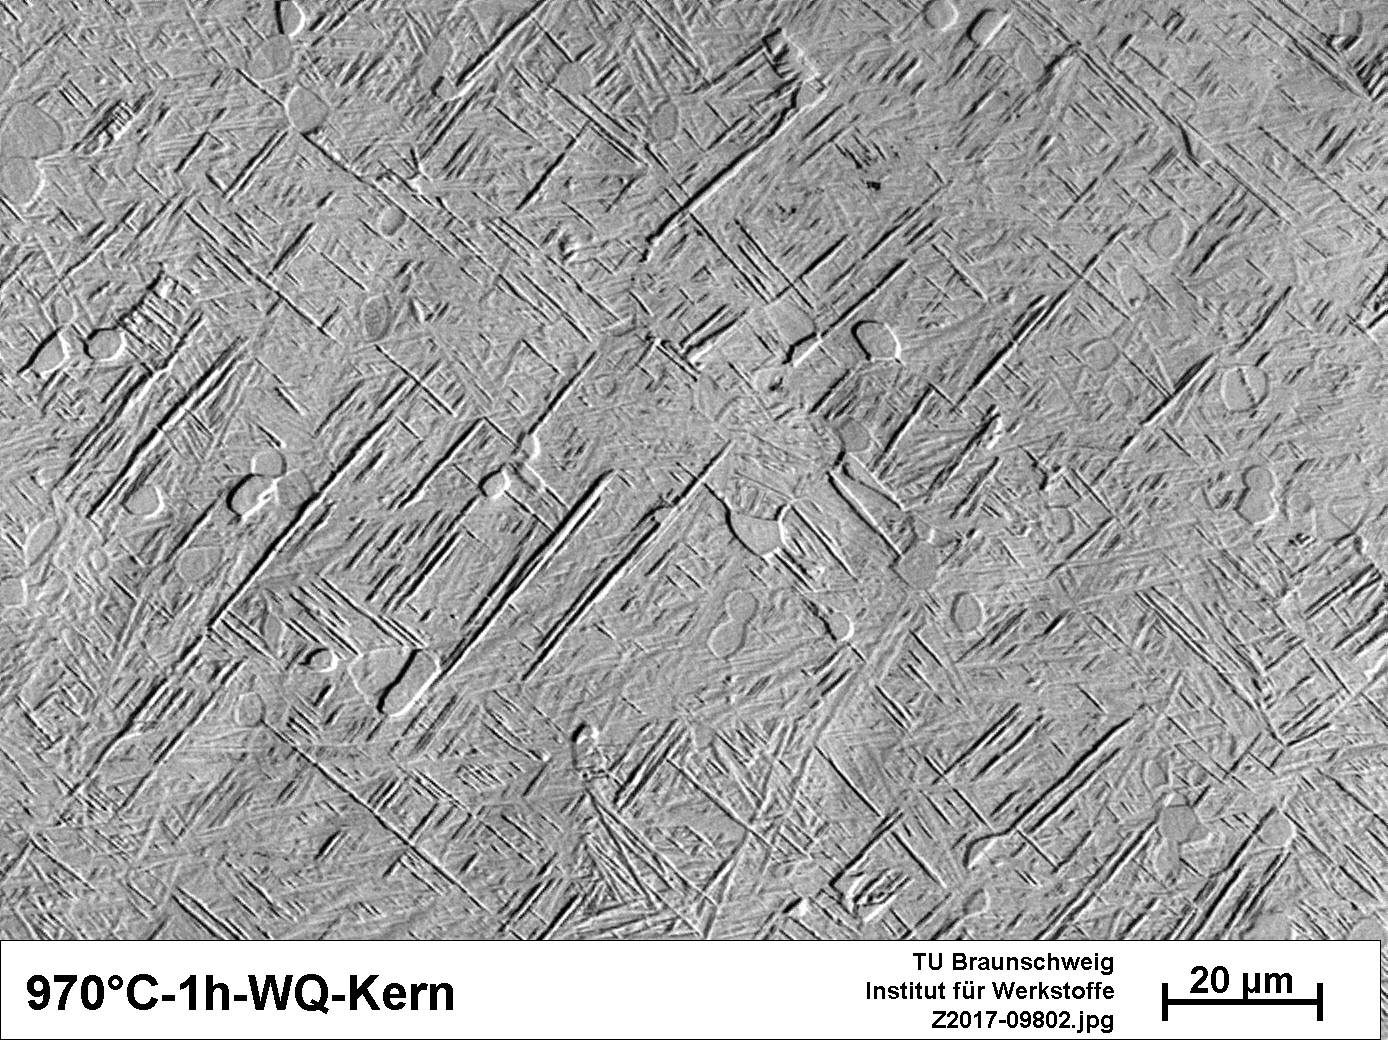
\includegraphics[width=0.33\textwidth]{Bilder/9701hwq.jpg}}
\subfigure[Gefüge bei einer Glühungstemperatur von 960°C]{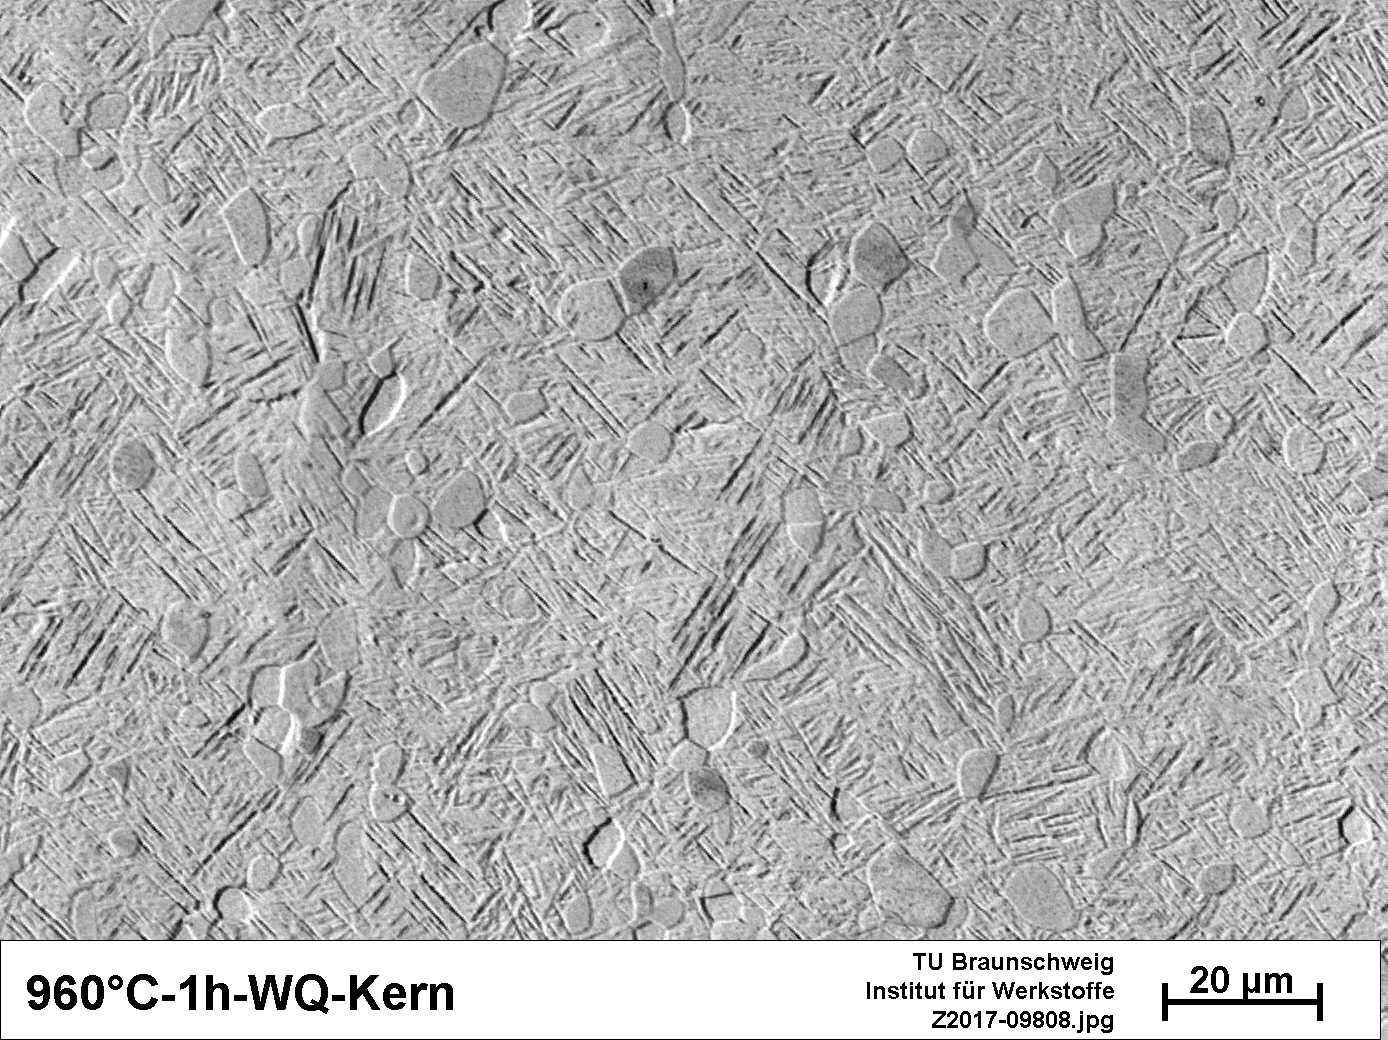
\includegraphics[width=0.33\textwidth]{Bilder/9601hwq.jpg}}
\subfigure[Gefüge bei einer Glühungstemperatur von 950°C]{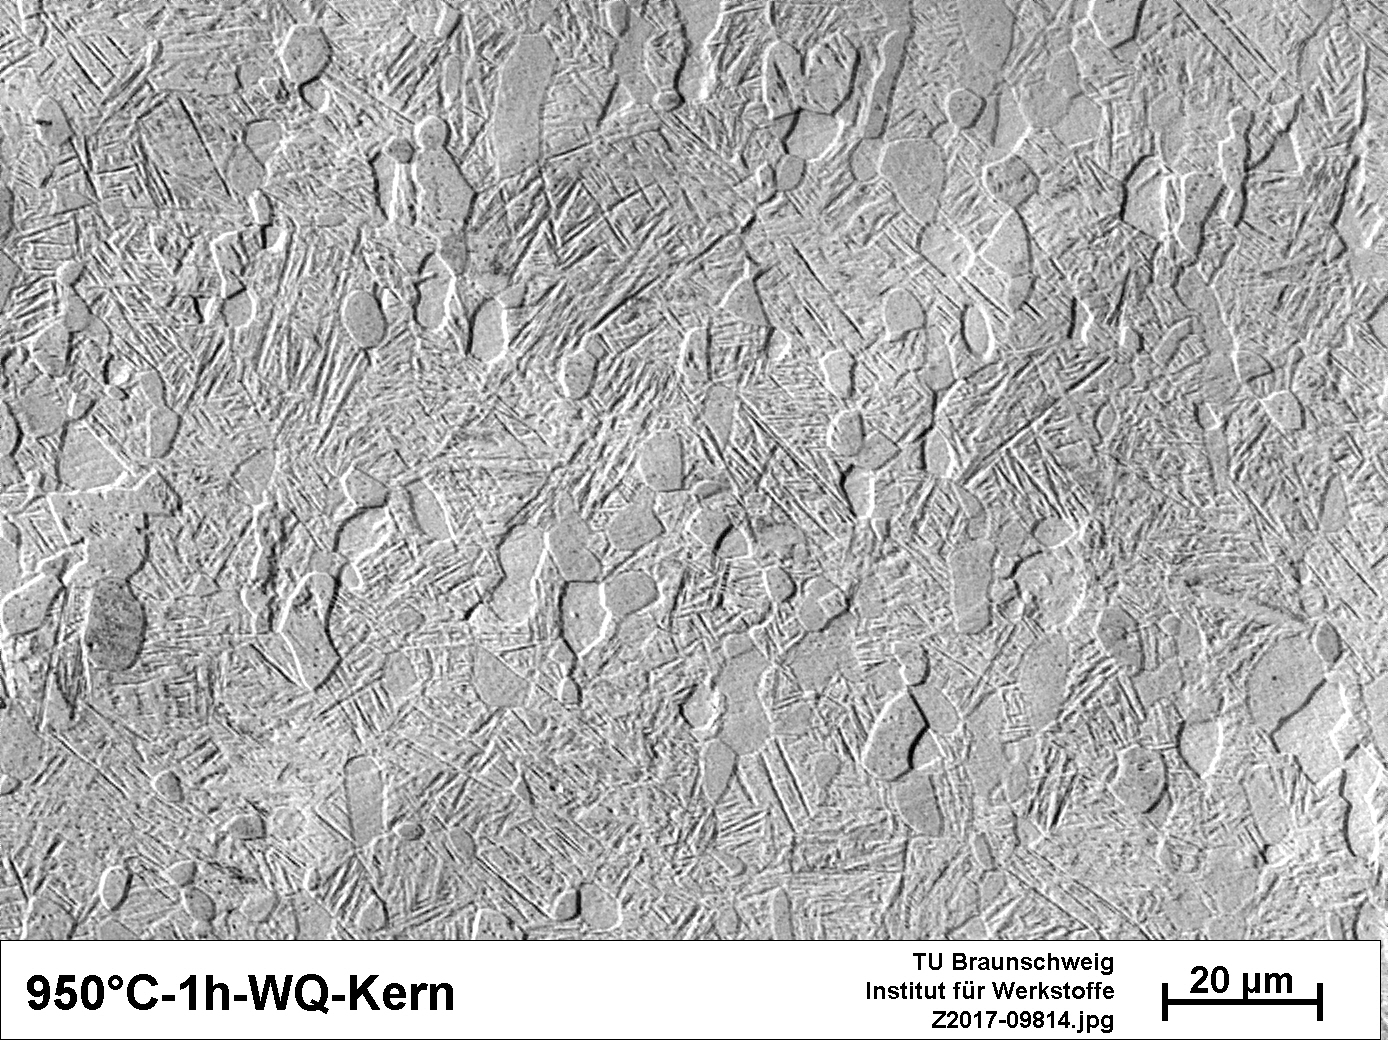
\includegraphics[width=0.33\textwidth]{Bilder/9501hwq.jpg}}
\caption{Primär Alpha-Martensit-Gefüge bei unterschiedlichen Glühtemperaturen}
\label{Alle Glühen}
\end{figure}

\newpage
\subsection{Abhängigkeit der Härte vom Primär-Alpha-Anteil} \label{Kapitel Abhängigkeit der Härte vom Primäralphaanteil}
Der Einfluss den der Alpha-Anteil auf die mechanischen Eigenschaften des Gefüges hat wird im Folgenden untersucht. Die Härteprüfung (siehe Kapitel \ref{Kapitel Härte}) dient hier als Hilfswert für die Festigkeitsabschätzung. Bei einer Prüfkraft von 10HV dringt der Prüfkörper in die Alpha Körner und den Martensit ein. Somit entsteht ein gemittelter Härtewert des Gefüges. Die Tabelle \ref{Härte in Abhängigkeit der Glühtemperatur} zeigt, dass mit sinkendem Alpha-Anteil die Härte zunimmt. Bei einem Anteil von ca. 20\% liegt der Härtewert bei 343 HV10. Die Härte steigt bei der Probe mit dem geringsten Alpha-Phasenanteil bis auf 357 HV10 an.



\subsection{Elementverteilung in den Phasen}
Die unterschiedliche Gewichtung der Phasenanteile im Gefüge wirkt sich auf die Verteilung der Legierungselemente aus. Mithilfe der EDX Analyse kann diese bestimmt werden (siehe Kapitel \ref{Kapitel EDX}). Die Abbildungen \ref{EDX Analyse der Phasen} zeigen die Analyse in einem Alpha-Korn und in der Martensit-Matrix. Die Elemente Titan, Aluminium und Vanadium werden für die Legierung Ti 6Al 4V berücksichtigt. Hierbei problematisch sind die charakteristischen Wellenlängen von Titan und Vanadium. Die einzelnen Peaks überlagern sich, sodass dem Titan ein gewisser Anteil Vanadium zugerechnet wird (siehe Abbildung \ref{Röntgenspektrum}). Der vorliegende Anteil an Vanadium ist höher als der Ermittelte. Aus mehreren Messungen wird der Mittelwert gebildet und die Verteilung kann dargestellt werden.

\begin{figure}
\subfigure[EDX Analyse im Alphakorn]{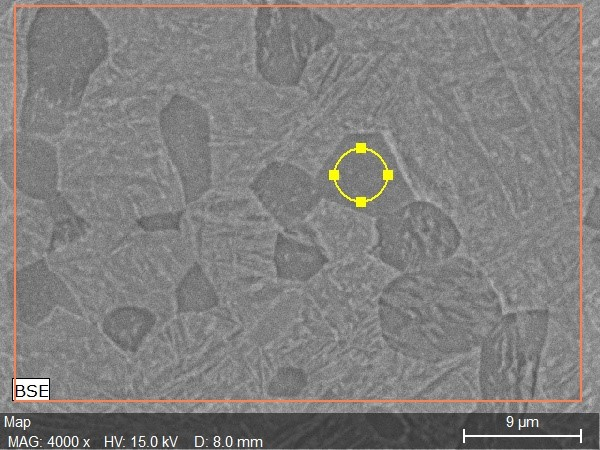
\includegraphics[width=0.4\textwidth]{Bilder/EDX1.jpg}}
\subfigure[EDX Analyse im Martensit]{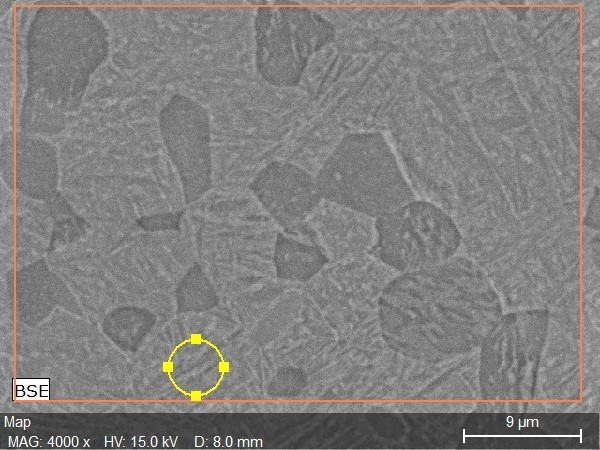
\includegraphics[width=0.4\textwidth]{Bilder/EDX2.jpg}}
\caption{EDX Analyse der Phasen}
\label{EDX Analyse der Phasen}
\end{figure}
\begin{figure}
\centering
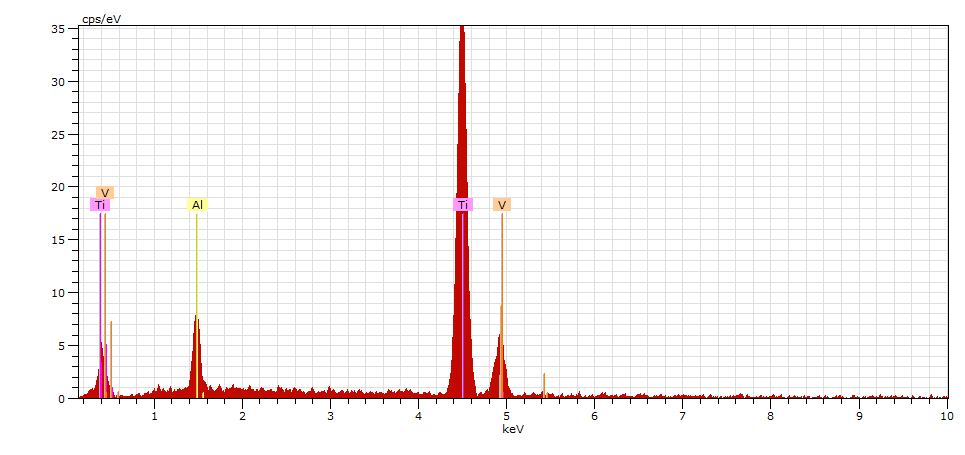
\includegraphics[width=0.66\textwidth]{Bilder/Roentgenspektrumti64.png}
\caption{Röntgenspektrum Ti 6Al 4V}
\label{Röntgenspektrum}
\end{figure}
\newpage
Die Tabelle \ref{Tabelle EDX Analyse} zeigt die Verteilung der Legierungselemente für die Proben mit einem Primär-Alpha-Anteil von 20\% und 6\%. Das Aluminium als Alpha-Stabilisator reichert sich in den Alpha-Körnern an. Mit sinkendem Alpha-Anteil ist ein größerer Anteil Aluminium im Korn gelöst. Die Löslichkeit des Vanadiums als Beta-Stabilisator im Alpha-Korn ist gering. Im metastabilen Martensit sind beide Stabilisatoren eingelagert, jedoch steigt der Vanadium-Anteil mit einem größeren Anteil der Alpha-Phase (siehe Kapitel \ref{Kapitel Diffusion von legierungselementen}).    
\begin{table}
\begin{tabular}{c|c|c|c|c}
Primär Alpha & \multicolumn{2}{c}{Primär Alpha Phase} & \multicolumn{2}{|c}{Martensit Phase} \\
\cline{2-5}
Anteil [\%] & Al [\%] & V[\%] & Al [\%] & V [\%] \\
\hline
20 & 5,90 & 0,31 & 5,31 & 2,11 \\
\hline
6 & 6,20 & 0,08 & 5,53 & 1,78 \\

\end{tabular}
\caption{EDX Analyse, Aluminium und Vanadium Anteile in Gewichtsprozent}
\label{Tabelle EDX Analyse}
\end{table}
\subsection{Bewertung der Ergebnisse}
Das eingestellte Gefüge, bestehend aus Primär-Alpha und Martensit besitzt eine größere Härte als der Ausgangszustand. Das Einstellen des Alpha-Anteils durch die Glühtemperatur führte zur Steigerung der Härte auf 357 HV10. Die Härte steigt mit sinkendem Anteil. Daraus resultiert die Frage, ob ein vollmartensitisches Gefüge eine noch größere Härte aufweist.

Die Variation der Phasenanteile hat einen Einfluss auf die Verteilung der Legierungselemente. Durch das ''element partitioning'' können sich große Anteile Aluminium im Alpha-Korn lösen oder der Anteil Vanadium im Martensit steigt. Diese Kenntnis über die Verteilung wird für das spätere Auslagern bzw. Altern benötigt. 

Die erzielten Ergebnisse korrelieren mit den Ergebnissen und Daten aus der Literatur. Aufbauend wird das Vollmartensitische Gefüge näher untersucht und eine Alterungsstrategie verfolgt.   

\newpage
\section{Festigkeitssteigerung durch Bildung und Zerfall des Vollmartensits (Jonas Veer)}\label{Kapitel Bildung und Zerfall des Vollmartensits}
Die Ergebnisse der ersten Wärmebehandlung zeigen, dass mit sinkendem Primär Alpha-Anteil die Härte steigt. Also sollte ein rein martensitisches Gefüge höhere Härtewerte aufweisen. 

Als Grundlage für die Strategie dienen die Quellen \cite{Mur1995} und \cite{Tarin1995}. In beiden Arbeiten wird ein vollmartensitisches-Gefüge erzeugt und anschließend der Zerfall von einem martensitischem Gefüge behandelt. Die Proben werden in der ersten Wärmebehandlung bei 1050°C für 30 Minuten geglüht und in Wasser abgekühlt um einen reinen Martensit einzustellen. Nach diesem Schritt besitzt die Probe eine Härte von 330 HV10. Im zweiten Schritt werden die Proben bei 400°C, 600°C, 700°C und 800°C und zu unterschiedlichen Haltezeiten geglüht um den Martensit in Alpha und Beta-Phase zerfallen zu lassen. 

\begin{figure}
\centering
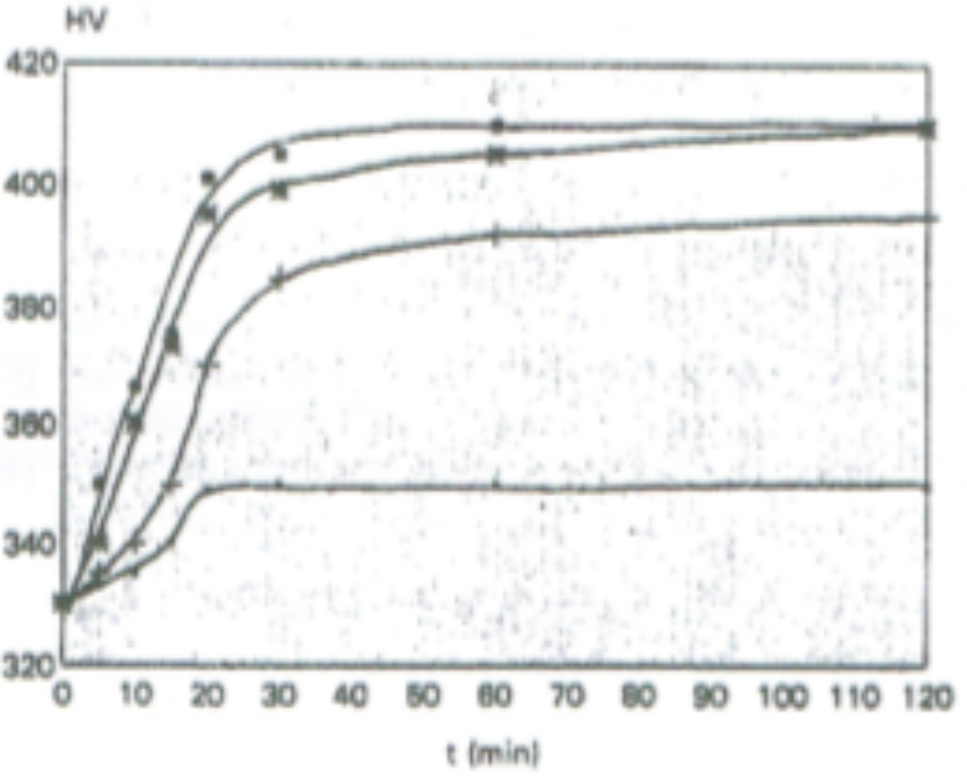
\includegraphics[width=0.5\textwidth]{Bilder/HaerteHaltezeitdiagramm.png}
\caption[Härte-Haltezeit Diagramm]{Härte-Haltezeit Diagramm für 400°C, 600°C, 700°C und 800°C \cite{Mur1995}}
\label{Härtehaltezeitdigramm}
\end{figure}

Die Abbildung \ref{Härtehaltezeitdigramm} zeigt, dass die Transformation der Martnesit-Phase zu Alpha- und Beta-Phase temperatur- und zeitabhängig ist. Die höchste Härte ergibt sich bei 800°C und einer Haltezeit von bis zu zwei Stunden. Sie liegt bei 410 HV10. Für 400°C ist erkennbar, dass die Umwandlung von Martensit zu Alpha- und Beta-Phase unvollständig ist und auch bei einer längeren Haltezeit nicht weiter voranschreitet. Die Härte erreicht nach ungefähr 30 Minuten bei 350 HV10 ihren Höhepunkt und bei längeren Zeiten nicht weiter ansteigt (siehe Abbildung \ref{Gefuegestruktur zweier Martensit Auslageungen}). Bei Temperaturen über 600°C schreitet die Transformation weiter voran, was sich auch in den Härtewerten von bis zu 410 HV10 wiederspiegelt. 

\subsection{Angestrebte Wärmebehandlung}
Aus den Quellen lässt sich schließen, dass eine zweistufige Wärmebehandlung aus Glühen bei 1050°C für 30 Minuten und einem Martensitzerfall bei 800°C für bis zu zwei Stunden eine hohe Härte und Festigkeit aufweist.

Um ein solches Gefüge einzustellen muss zunächst über der Betatransus Temperatur geglüht werden, sodass eine vollständige Umwandlung von Alpha- zu Beta-Phase stattfindet. Bei hohen Glühtemperaturen wird das Kornwachstum zu einem Problem. Die Temperatur sollte nur für eine kurze Zeit gehalten und so niedrig wie möglich gewählt werden. Auf Grund von unterschiedlichen Werten der Betatrasus Temperatur, die in der Literatur bei bis zu 1020°C liegt\cite{Tarin1995}, werden die Proben bei 1050°C geglüht und im Nachhinein mit Wasser abgeschreckt. Um das Kornwachstum zu steuern betragen die Haltezeiten 10 min und 30 min. 


Ziel ist es durch die Martensitplatten eine hohe Grenzflächendichte zu erzeugen und im zweiten Schritt diese Platten zu unterteilen, sodass der Martensit durch Zwillinge unterbrochen wird, was in Abbildung \ref{Gefuegestruktur zweier Martensit Auslageungen}(b) zu sehen ist, und so die Versetzungsbewegung durch die Martensit-Phase zu stören.

\begin{figure}
\subfigure[Gefügestruktur einer Probe geglüht bei 400°C für 60min]{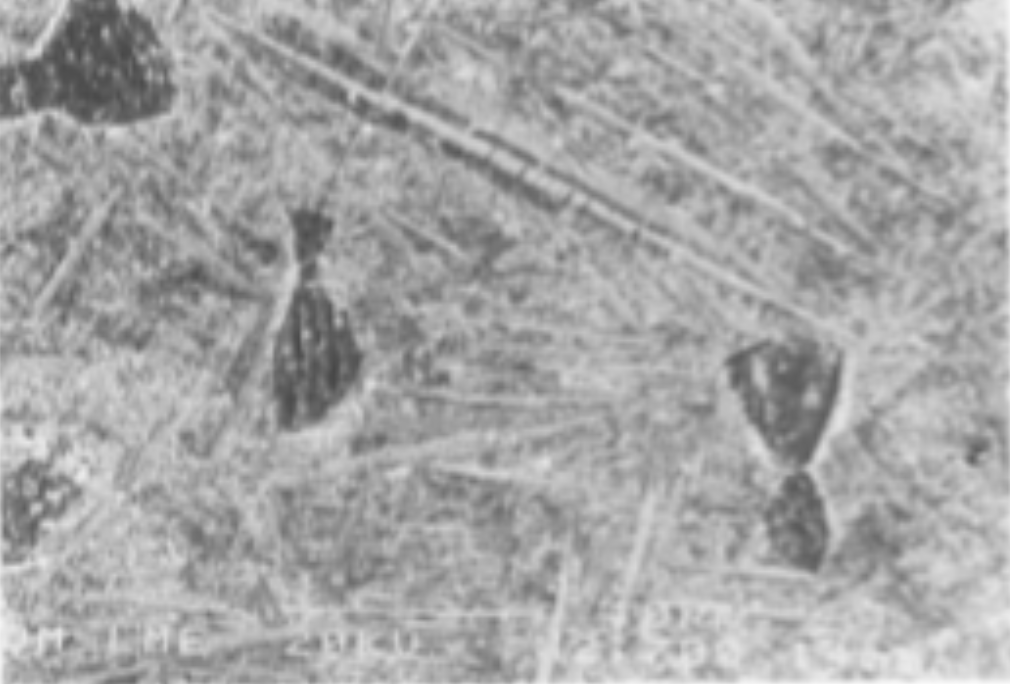
\includegraphics[width=0.5\textwidth]{Bilder/Gefuegestruktur4001h.png}}
\subfigure[Gefügestruktur einer Probe geglüht bei 700°C für 30min]{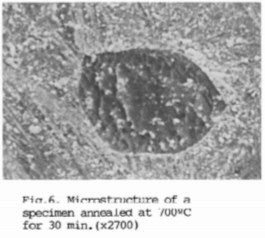
\includegraphics[width=0.5\textwidth]{Bilder/Gefuegestruktur70030min.png}}
\caption{Gefüge zweier Martensit-Auslagerungen}
\label{Gefuegestruktur zweier Martensit Auslageungen}
\end{figure}




\subsection{Ergebnisse und Bewertung der Wärmebehandlungen}
Es zeigt sich in der lichtmikroskopischen Untersuchung, dass der Einfluss der Glühzeiten auf das Beta-Kornwachstum sehr gering ist, da die Korngrößen im Martensit bei beiden Proben etwa bei 600 $\mu$m liegen (siehe Abbildung \ref{Korngroessenbestimmung Martensit}). Auch die Härtewerte sind mit 342HV10 (30min) und 346HV10 (10min) ungefähr gleich. 


\begin{figure}
\subfigure[1050°C 30min Wasser abgeschreckt]{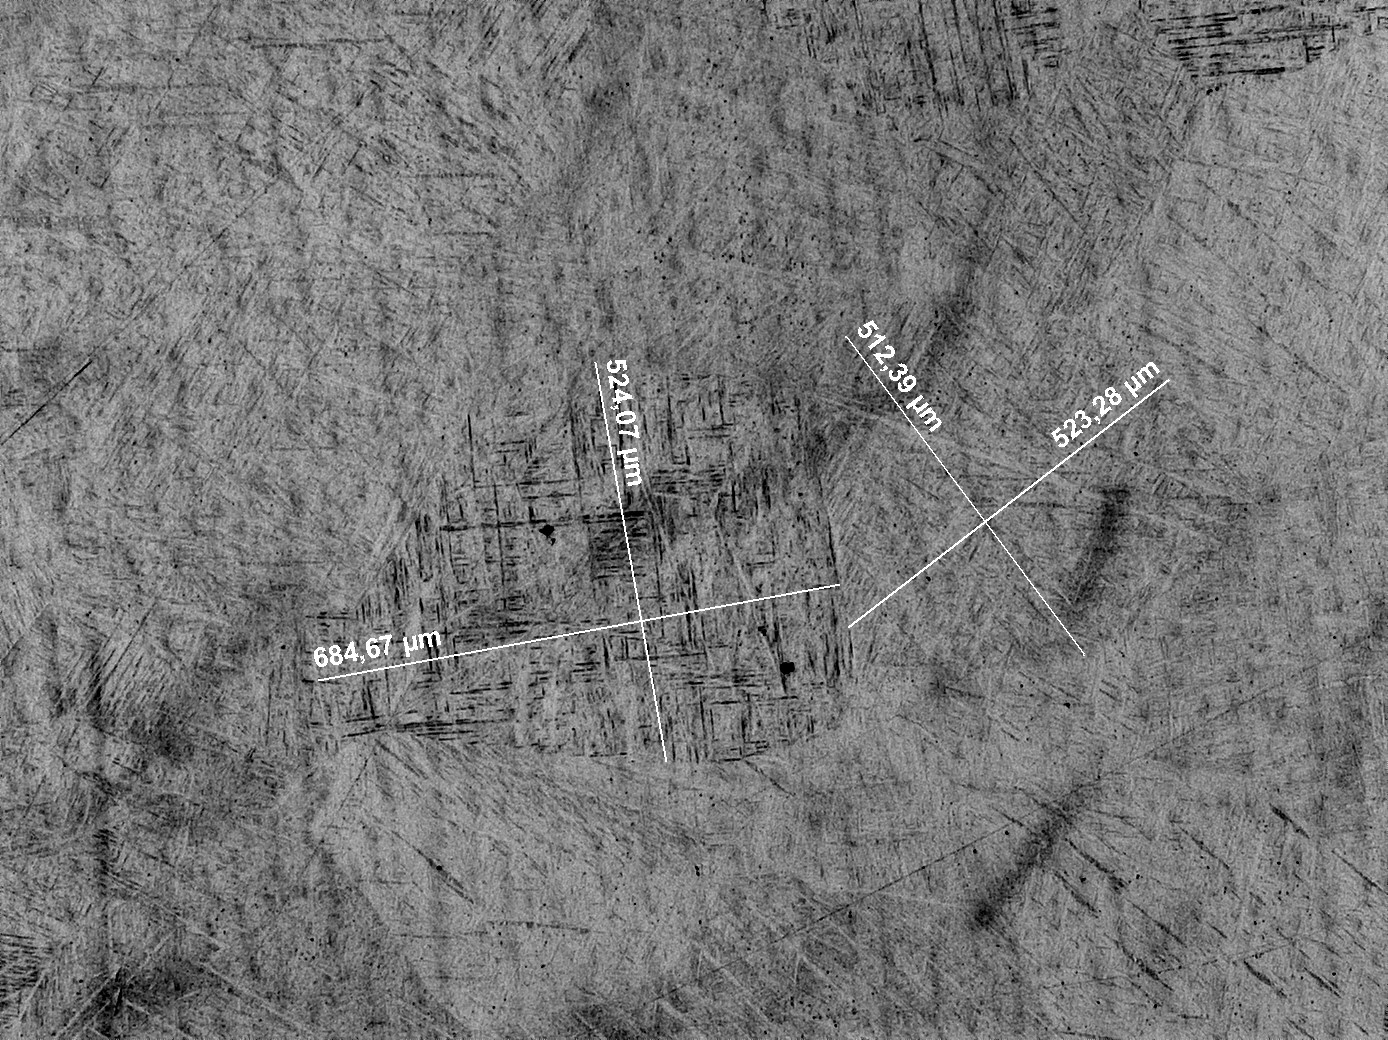
\includegraphics[width=0.5\textwidth]{Bilder/Korngroessemartensit.jpg}}
\subfigure[1050°C 10min Wasser abgeschreckt]{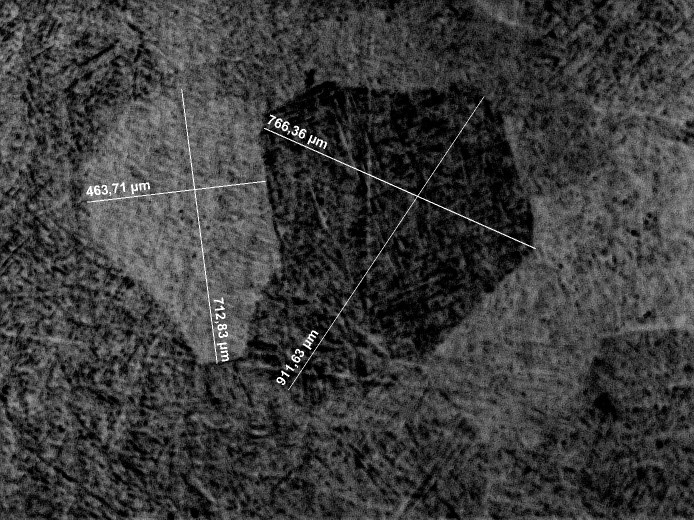
\includegraphics[width=0.5\textwidth]{Bilder/Korngroessemartensit1.jpg}}
\caption{Korngrößenbestimmung der ehemaligen Betakörner im Martensit}
\label{Korngroessenbestimmung Martensit}
\end{figure}

\newpage
Die Härtesteigerung um ca. 40 HV10 im Vergleich zum Ausgangsgefüge entsteht durch eine erhöhte Grenzflächendichte. Anders als im Eisen, in dem die Zwangslösung von Kohlenstoffatomen in einem tetragonal-raumzentrierten Gitter eine festigkeitssteigernde Wirkung hat, kommt es im martensitischem Titan nur marginal zu Gitterverzerrung durch die Zwangslösung von Vanadium in der Alpha-Phase die keinen Einfluss auf die Festigkeit hat. Entgegen der Erwartungen ist die Härte im Gegensatz zum Primären-Alpha-Martensit-Gefüge nicht weiter gestiegen, sondern ist um ca. 10 - 15 HV10 niedriger als die Probe 970°C-1h-WQ. Zu erklären ist das durch die langen Martensit-Nadeln, welche nicht mehr durch Primär-Alpha-Körner unterbrochen werden (siehe Abbildung \ref{Auslagerung des Vollmartensits}).
Bei den geglühten Proben ergibt die Härtemessung Werte von 325 HV10. Dieses Ergebnis liegt 20 HV10 unter dem reinen Martensit-Gefüge und 85 HV10 unter der Härte aus den Quellen.
Abbildung \ref{vergleich vollmartensit und auslagerung} zeigt, dass die Probe im ausgelagertem Zustand Grenzflächen verloren hat. Das Gefüge ist hat sich vergröbert. Die feinen Platten des Martensits sind in eine Gleichgewichtsphase aus Alpha und Beta zerfallen. 

\begin{figure}
\subfigure[Vollmartensit-Gefüge]{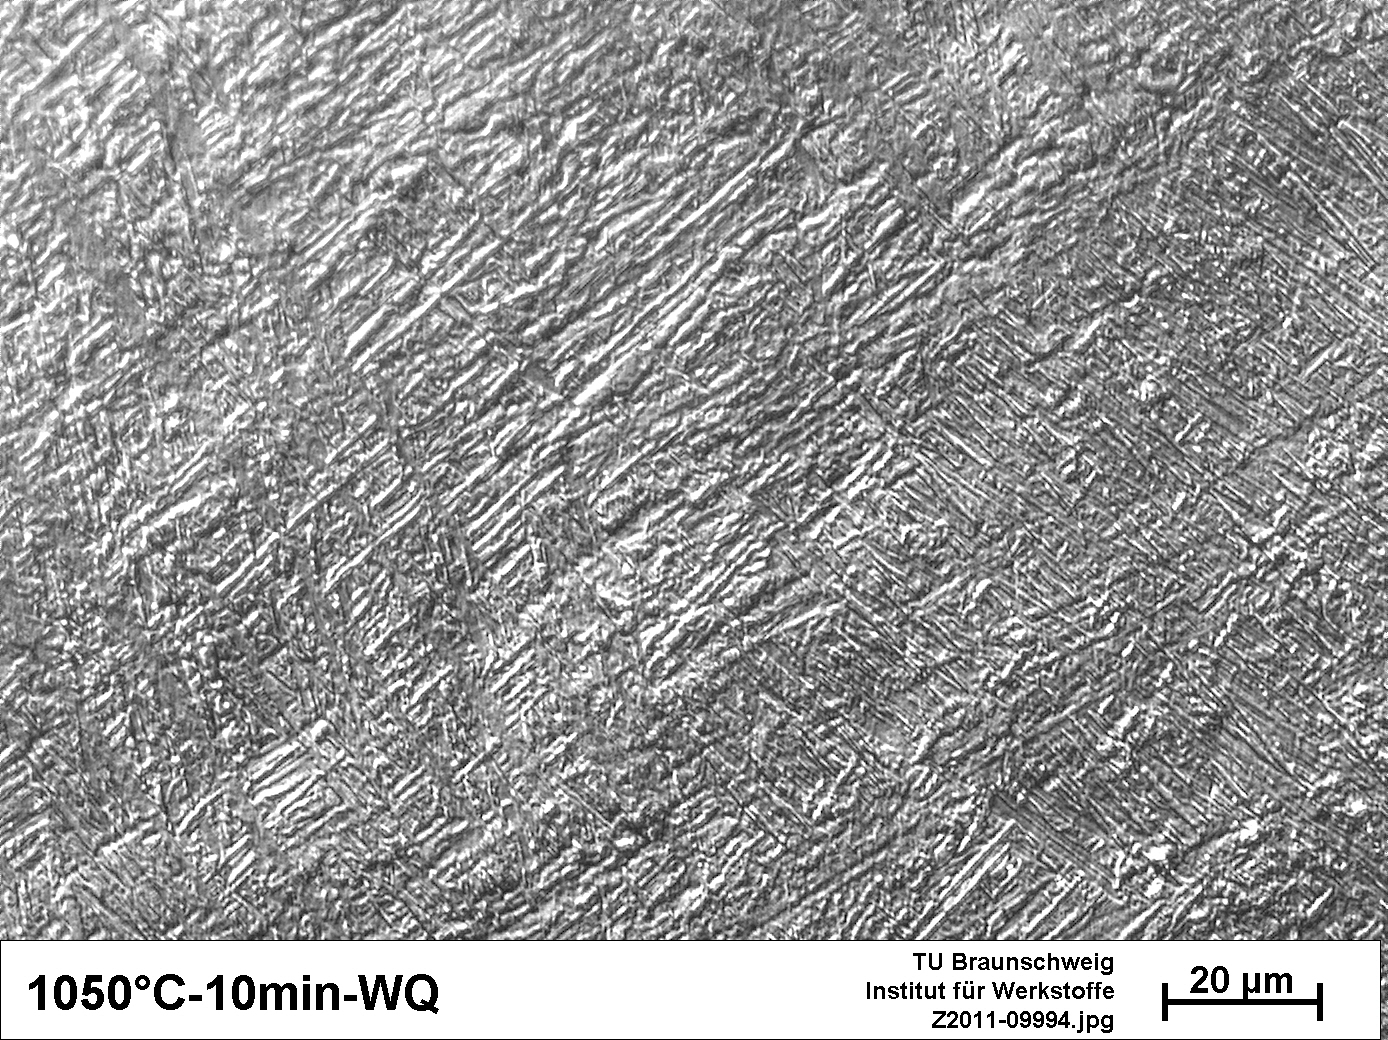
\includegraphics[width=0.5\textwidth]{Bilder/105010minwq.jpg}}
\subfigure[Ausgelagertes Vollmartensit-Gefüge]{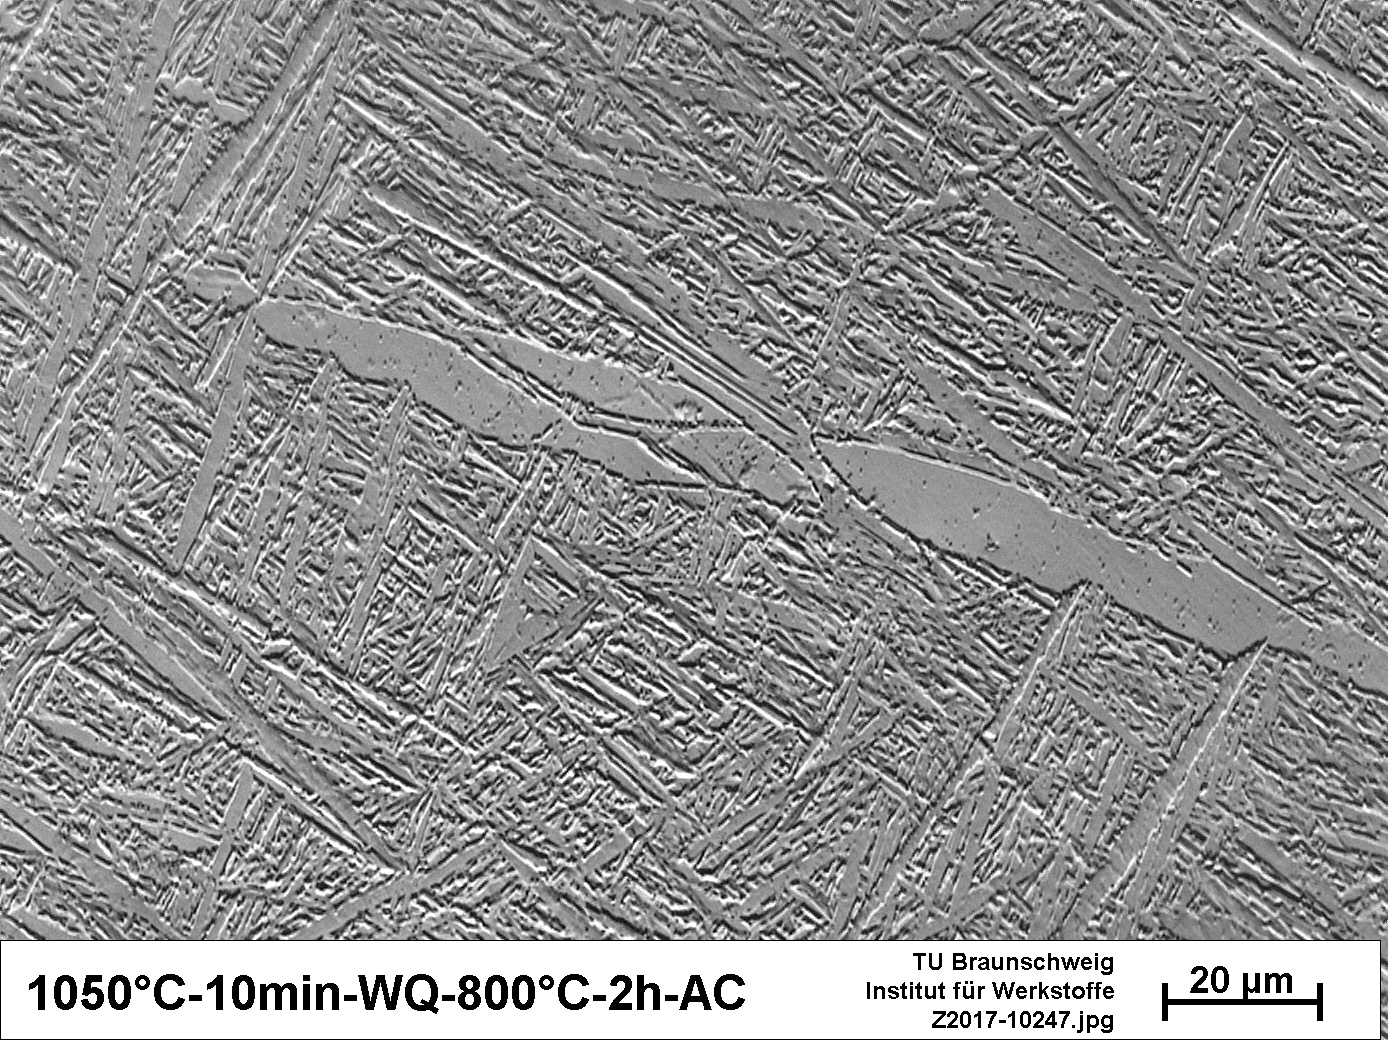
\includegraphics[width=0.5\textwidth]{Bilder/105010minwq8002hac.jpg}}
\caption{sichtbare Vergröberung des Zerfalls der Vollmartensit-Phase}
\label{vergleich vollmartensit und auslagerung}
\end{figure}
In Abbildung \ref{Auslagerung des Vollmartensits} ist der Vollmartensit im Vergleich zu der ausgelagerten Probe unter dem REM dargestellt. Der Martensit ist vollständig in die Alpha- und Beta-Phase zerfallen und es sind keine Martensit-Nadeln mehr zu erkennen. Die Alpha-Phase ist zu großen Körnern angewachsen. In diesen sind hellere Bereiche entstanden, welche aus Beta-Phase bestehen.

\begin{figure}
\subfigure[Probe Vollmartensit]{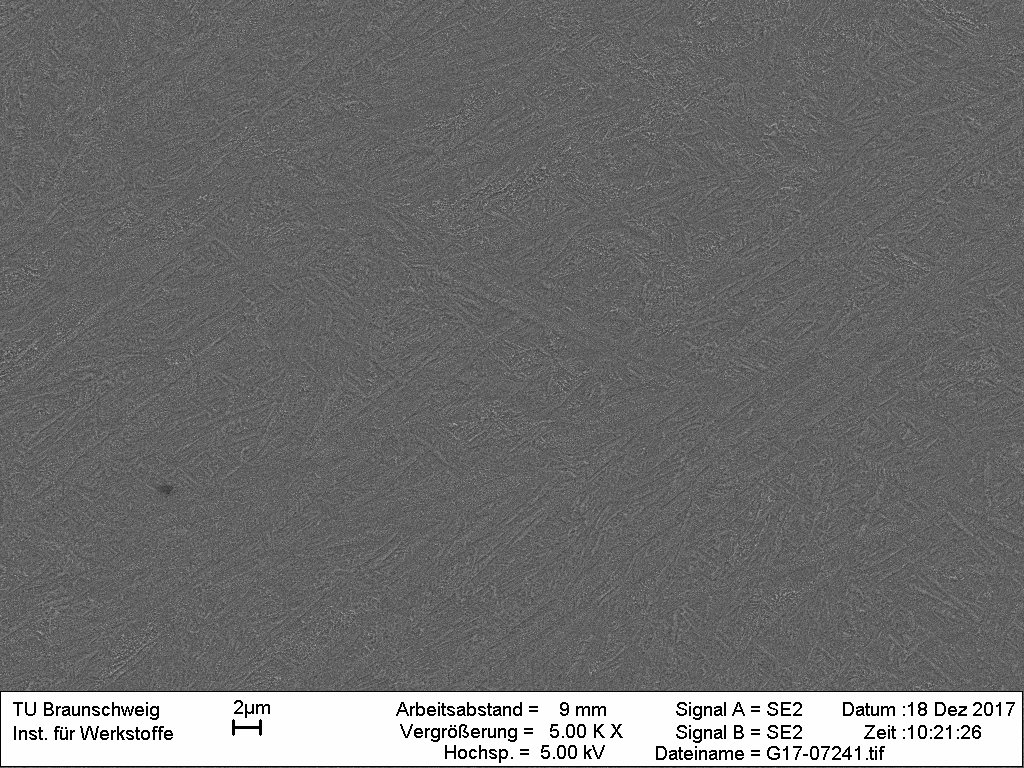
\includegraphics[width=0.5\textwidth]{Bilder/REMVollmartensit.jpg}}
\subfigure[Probe Martensitzerfall]{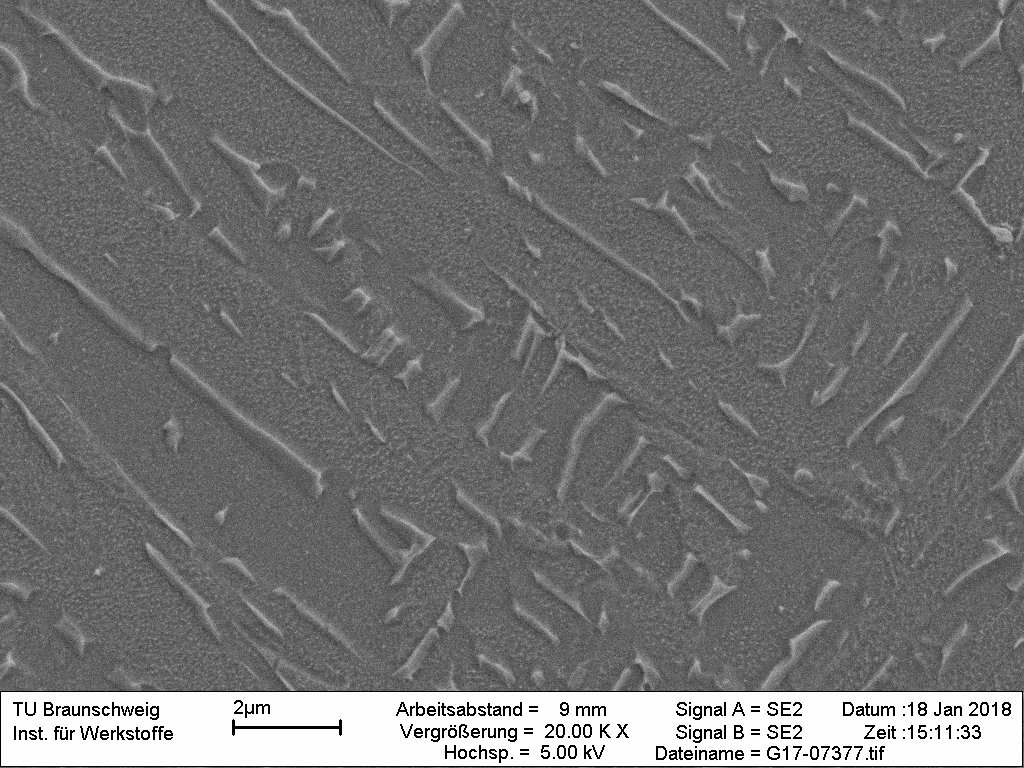
\includegraphics[width=0.5\textwidth]{Bilder/REMVollmartensitzerfall.jpg}}
\caption{Auslagerung des Vollmartensits}
\label{Auslagerung des Vollmartensits}
\end{figure}

\newpage


\section{Festigkeitssteigerung durch Auslagern von Primäralpha und Martensit (Tammo Stein)}\label{Primäralpha und martensit}
In zahlreichen vergleichbaren Untersuchungen wurde bereits eine Festigkeitssteigerung durch Auslagerung von primär Alpha-Martensit-Gefügen festgestellt. Auf Basis dieser Untersuchungen und von Ergebnissen der Wärmebehandlung aus Kapitel \ref{Festigkeitssteigerung durch Martensitbildung} werden die Parameter für diese Wärmebehandlung gewählt. Ziel dieser Behandlung ist, den metastabilen Martensit in sekundäre Alpha- und Beta-Phase zerfallen zu lassen. Die so entstehenen kleinen Bereiche sollen die mechanischen Eigenschaften beeinflussen und die Festigkeit erhöhen\cite{Gilbert2004}. Es konkurrieren jedoch zwei Mechanismen bei einer Alterung des Martensits. 

Zum einen werden die Nadeln innerhalb des Martensits breiter, sodass eine Abnahme der Härte aufgrund geringerer Grenzflächendichte folgt. Der andere Mechanismus ist der Zerfall des Martensits in feine Alpha- und Betakörner die sich innerhalb des Gefüges bilden. Diese feinen Körner sorgen für eine Festigkeitssteigerung. Es ist also das Ziel, die Vergröberung des Gefüges zu minimieren, während der Zerfall maximiert werden soll. 
\subsection{1. Wärmebehandlerung: Auslagerung mit dem Ziel eines zerfallenen Martensit}
Wärmebehandlungen wie in den Quellenangaben \cite{Gilbert2004} und \cite{Chen2008} geben Beispiele für erfolgreiche Glüh- und Alterungsprozesse. Sie dienen als Hilfsmittel für die Parameterwahl bei dieser Wärmebehandlung. Bei den Bespielen werden Glühtemperaturen von 950°C bis 970°C verwendet, sodass ein zweiphasiges Gefüge mit unterschiedlichen Primäralpha-Gehalten entsteht (siehe Kapitel \ref{Festigkeitssteigerung durch Martensitbildung}). 

Wie die Wärmebehandlung aus Kapitel \ref{Festigkeitssteigerung durch Martensitbildung} zeigt, wirkt sich ein geringer Primäralpha Anteil positiv auf die Härte beziehungsweise Festigkeit aus. Für den Zerfall des Martensits ist jedoch die Konzentration an Beta stabilisierender Elemente in der Martensit-Phase entscheidend. Eine hohe Konzentration an Vanadium in der Martensit-Phase wird angestrebt. Diese liegt nach den EDX-Ergebnissen aus Kapitel \ref{Festigkeitssteigerung durch Martensitbildung} niedriger, je kleiner der Primäralpha-Anteil ist. Demnach sind Proben mit einem höheren Primär Alpha-Anteil für eine Alterung besser geeignet \cite{Luetjering2007}.

Für die Alterung, mit anschließender Luftkühlung, wurde in den Behandlungen aus den Quellen eine Temperatur von 490°C bis 595°C und eine Haltezeit von 1 bis 8 Stunden angegeben. Da diese Spanne sehr groß ist und eine aussagekräftige Beurteilung der Ergebnisse für den gesamten Bereich unverhältnismäßig aufwendig sein würde, wurde eine Temperatur festgelegt und über die Haltezeit variiert.

So werden in einem ersten Schritt die Auswirkungen der unterschiedlichen Konzentrationen an Vanadium analysiert. Es wurden Wasser abgeschreckte Proben bei einer Glühtemperatur von 970°C und 950°C jeweils zwei und acht Stunden bei 520°C gealtert. So wird der größte und geringste Vanadium-Anteil berücksichtigt. Es werden also vier Proben verwendet, die ein vergleichbares Ergebnis liefern sollen. So kann eine Auswirkung der unterschiedlichen Vanadium-Konzentrationen gleichzeitig mit der Auswirkung der Haltedauer beobachtet werden und Rückschlüsse auf die entstehenden Eigenschaften getroffen werden.
\subsection{Ergebnisse der Auslagerung}
\subsubsection{970°C Auslagerung}
Auf den Gefügebildern mit dem Lichtbildmikroskop aus Abbildung \ref{970 alterung} sind kaum Unterscheide zu dem Ausgangsgefüge aus Abbildung \ref{Gefüge ohne Alterung}(a) zu sehen. Die Primäralpha Phase ist unabhängig von der Auslagerungszeit in ihrer Ausdehnung konstant geblieben. Der Martensit hat sich unter dem Lichtmikroskop nicht verändert. Falls die Martensit-Phase sich in ihrer Struktur verändert hat, ist dies nur unter einem REM zu sehen. Ein Zerfall würde sich nur in kleinen Bereichen äußern, die in dieser Vergrößerung nicht zu sehen sind. 


Die REM-Aufnahme aus Abbildung \ref{REM 970C und 950C}(a) zeigt das Gefüge von einem Abschrecken von 970°C. Wird diese Aufnahme mit denen nach dem Altern aus Abbildung \ref{REM 970C auslagerung} verglichen, fallen Unterschiede auf. Der gealterte Martensit hat eine ungleichmäßigere, ''körnigere''  Struktur als der nicht ausgelagerte. Diese Struktur ist bei der Probe mit längerer Haltezeit noch gröber. Zusätzlich hat sich an den Grenzflächen ein weißer Saum gebildet.
\begin{figure}
\subfigure[Glühen bei 970°C]{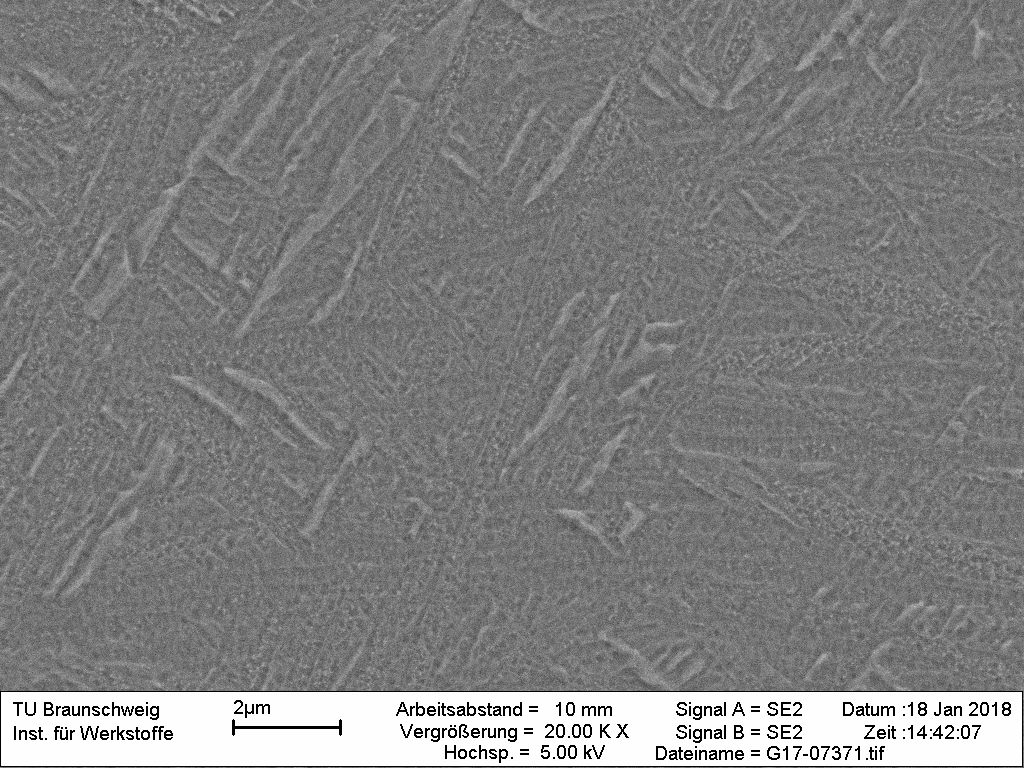
\includegraphics[width=0.5\textwidth]{Bilder/REM970C1hWQ.png}}
\subfigure[Glühen bei 950°C]{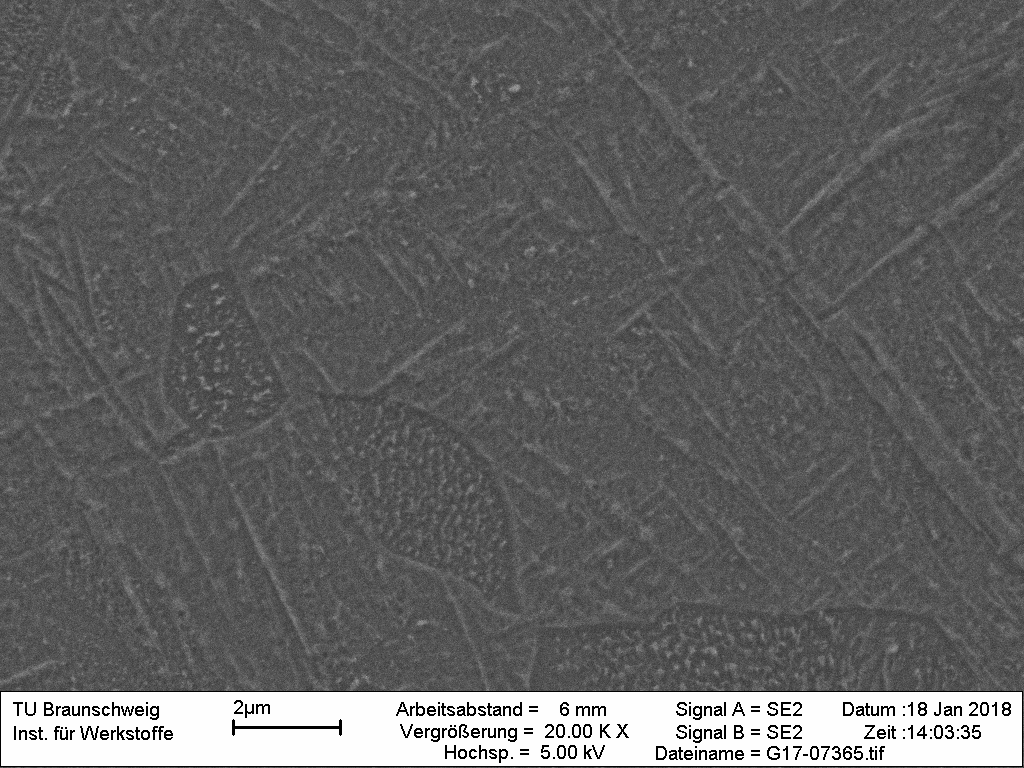
\includegraphics[width=0.5\textwidth]{Bilder/REM950C1hWQ.png}}
\caption{REM Bilder abschrecken von 950°C und 970°C}
\label{REM 970C und 950C}
\end{figure}


\begin{figure}
\subfigure[Zwei Stunden Alterung]{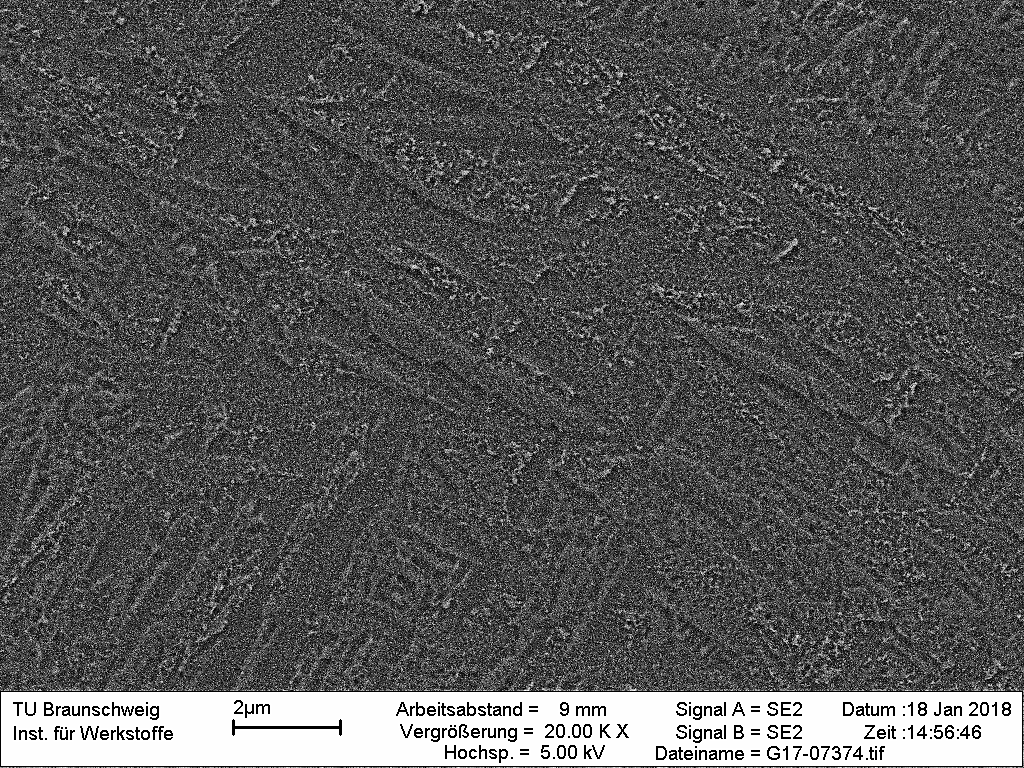
\includegraphics[width=0.5\textwidth]{Bilder/REM970C1hWQ520C2hAC.png}}
\subfigure[acht Stunden Alterung]{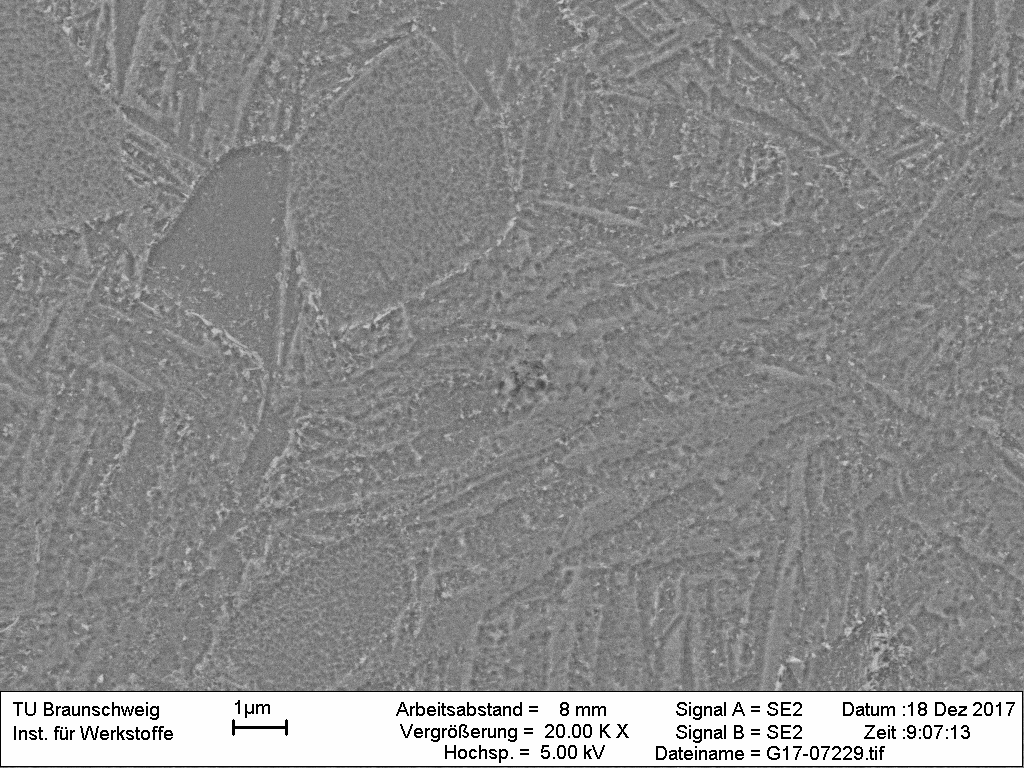
\includegraphics[width=0.5\textwidth]{Bilder/REM970C1hWQ520C8hAC.png}}
\caption{Gefüge der gealterten Proben Glühen bei 970°C}
\label{REM 970C auslagerung}
\end{figure}


Durch eine Härteprüfung lässt sich die Auswirkung der Alterung analysieren. Dabei wird das in Kapitel zwei beschriebene Verfahren angewendet. Für die Behandlungsreihe mit 970°C ergeben sich die Ergebnisse aus Tabelle \ref{heartepruefung970 inkl auslagern}. Ein Vergleich mit den Härtewerten der nicht ausgelagerten Probe aus Tabelle \ref{Hearte ohne Behandlung} zeigt keine Härtesteigerung. 
\subsubsection{950°C Auslagerung}
Wie auch schon bei den Proben bei 970°C sind unter dem Lichtmikroskop keine Unterschiede zwischen den ausgelagerten Proben und der unbehandelten Probe zu erkennen. Für eine genauere Analyse muss also ein REM herangezogen werden.

Die Bilder des REM aus Abbildung \ref{REM 950 2 und 8} zeigen das resultierende Gefüge nach den jeweiligen Haltezeiten. Es sind ähnliche Ergebnisse wie bei der Alterung der Glühtemperatur von 970°C zu erkennen. Der Martensit hat seine Struktur verändert. Die nach dem Abschrecken entstandenen Nadeln sind nur noch in kleinen Mengen zu sehen. Ein Großteil ist in vielen Stellen unterbrochen und gröber geworden. Die Struktur ist mit der Zeit noch gröber geworden und die Anzahl der Unterbrechungen ist größer geworden. Auch hier hat sich an den Grenzflächen ein weißer Saum gebildet,  jedoch ist dieser stärker ausgeprägt.
\begin{figure}
\subfigure[2 Stunden Haltezeit]{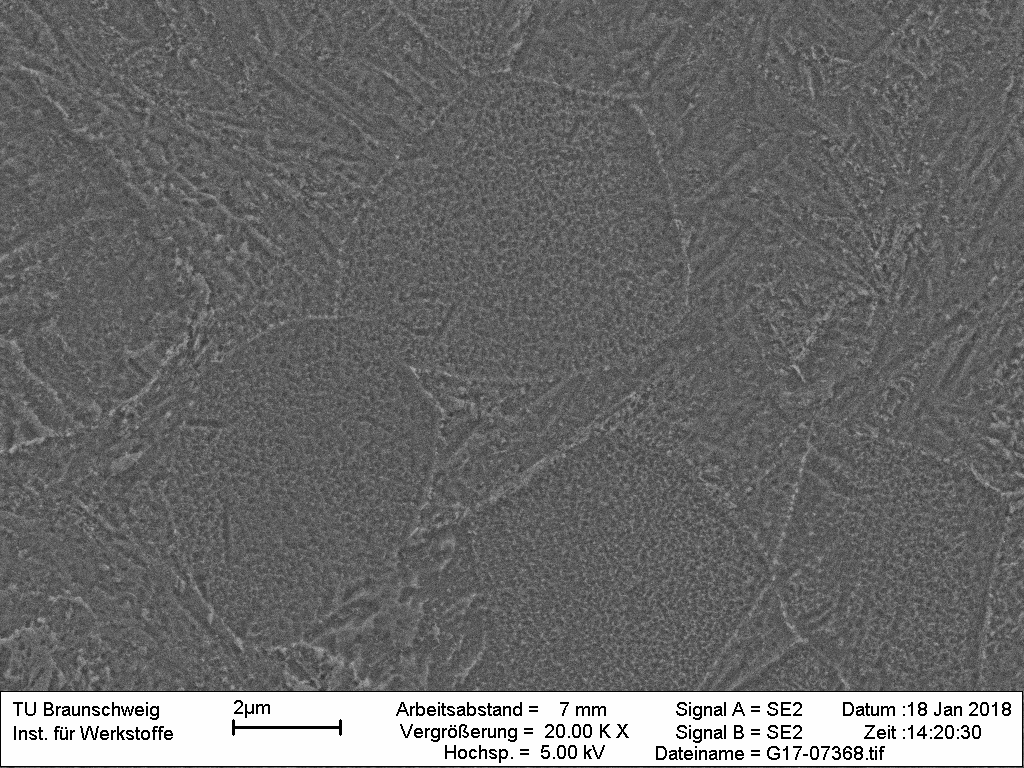
\includegraphics[width=0.5\textwidth]{Bilder/REM9501hWQ520C2hAC.png}}
\subfigure[8 Stunden Haltezeit]{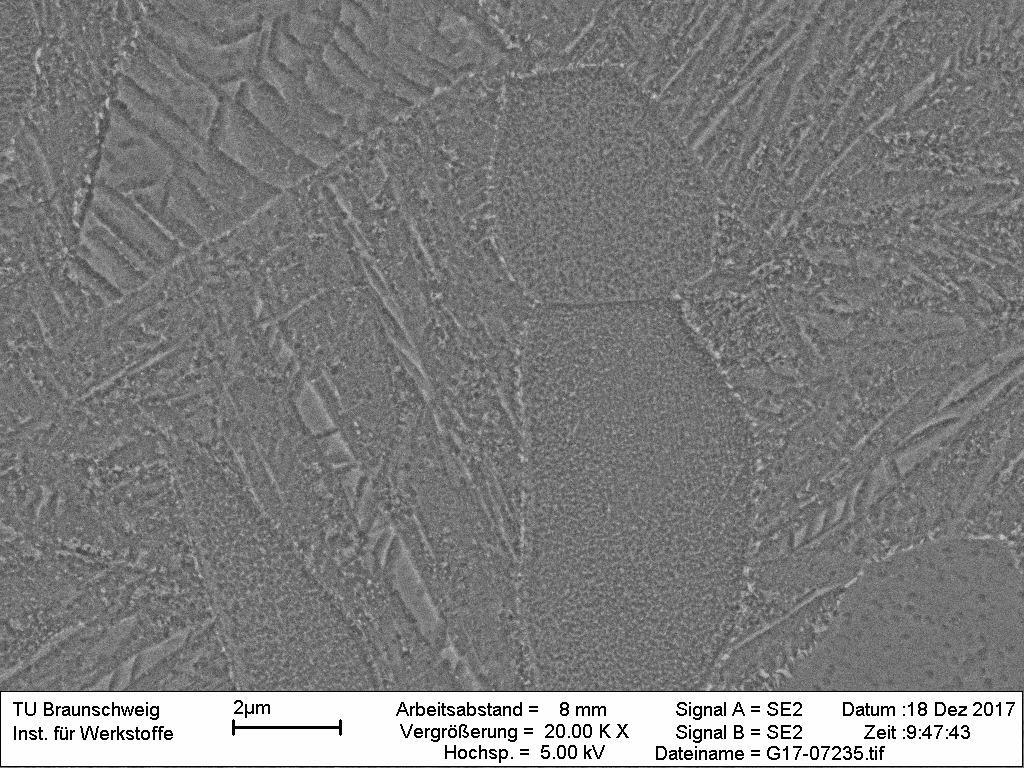
\includegraphics[width=0.5\textwidth]{Bilder/REM950C1hWQ520C8hAC.png}}
\label{REM 950 2 und 8}
\caption{Auslagerung der Glühtemperatur 950°C bei 2 und 8 Stunden}
\end{figure}

Bei den Proben, die mit 950°C geglüht und zwei beziehungsweise acht Stunden bei 520°C ausgelagert wurden, zeigt sich ein anderes Ergebnis der Härteprüfung als bei den Proben bei einer Glühtemperatur von 970°C. Wenn die Härtewerte nach der Alterung mit denen vorher verglichen werden, ist eine Härtesteigerung erkennbar. Die Werte aus der Tabelle \ref{950alterung} sind im Schnitt 10 HV10 höher als das Material vor der Behandlung. Die verwendeten Haltezeiten weisen keinen Unterschied hinsichtlich der Härte auf. Sie liegen für beide Zeiten bei circa 360 HV 10.
\begin{table}[t]	%Härtewerte ohne Auslagerung
\begin{tabular}{c|c|c}
Wärmebehandlung & Mittelwert in HV10 & Standardabweichung \\
\hline 
970°C 1h WQ	& 357 & 8,95\\
\hline
950°C 1h WQ & 343 & 6,68 \\


\end{tabular}
\caption{Härtewerte ohne Auslagerung}
\label{Hearte ohne Behandlung}
\end{table}
\begin{table}[t] 	%Härteprüfung 970°C Glühen und Auslagern
\begin{tabular}{c | c | c}
Haltezeit & Härte in HV10 & Standardabweichung \\
\hline
zwei Stunden & 358 & 2,58 \\
\hline
acht Stunden & 354 & 2,40 \\


\end{tabular}
\caption{Härteprüfung 970°C Glühen und Auslagern}
\label{heartepruefung970 inkl auslagern}
\end{table}
\begin{table}[t] 	%950 Alterung
\begin{tabular}{c|c}
\multicolumn{2}{c}{2h Auslagern} \\
\hline
Abstand in mm	& Härte in HV10 \\
0.01	&	352 \\
2.98	&	356 \\
5.94	&	356 \\
8.90	&	355 \\
11.86	&	358 \\
\hline
Mittelwert	&	355 \\
Max	&	358 \\
Min.	&	352 \\
Std.-abw.	&	2.43 \\

\end{tabular}
\begin{tabular}{c|c}
\multicolumn{2}{c}{8h Auslagern} \\
\hline
Abstand in mm	&	Härte in HV10 \\
0.02	&	357 \\
3.22	&	355 \\
6.42	&	358 \\
9.62	&	357 \\
12.82	&	354 \\
\hline
Mittelwert	&	356 \\
Max	&	358 \\
Min.	&	354 \\
Std.-abw.	&	1.83 \\

\end{tabular}
\caption{Härteprüfung 950°C Glühen und Auslagern}
\label{950alterung}
\end{table}
\begin{figure} 		%Gefüge Ohne Alterung
	\subfigure[Gefüge bei einer Glühungstemperatur von 970°C ohne Alterung]{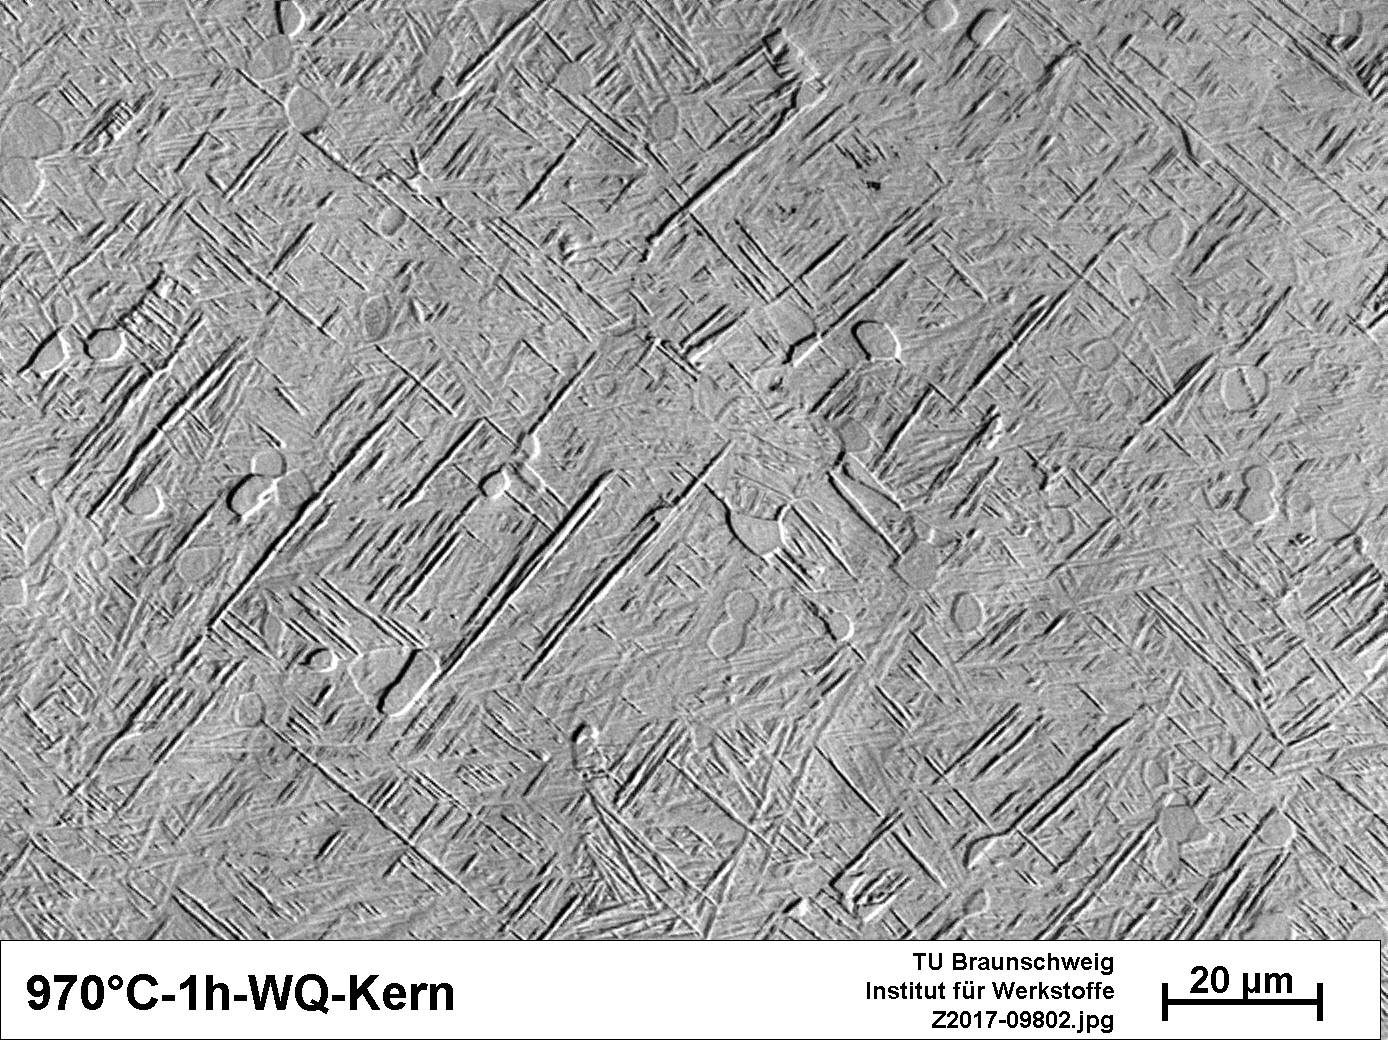
\includegraphics[width=0.49\textwidth]{Bilder/9701hwq.jpg}} 
    \subfigure[Gefüge bei einer Glühungstemperatur von 950°C ohne Alterung]{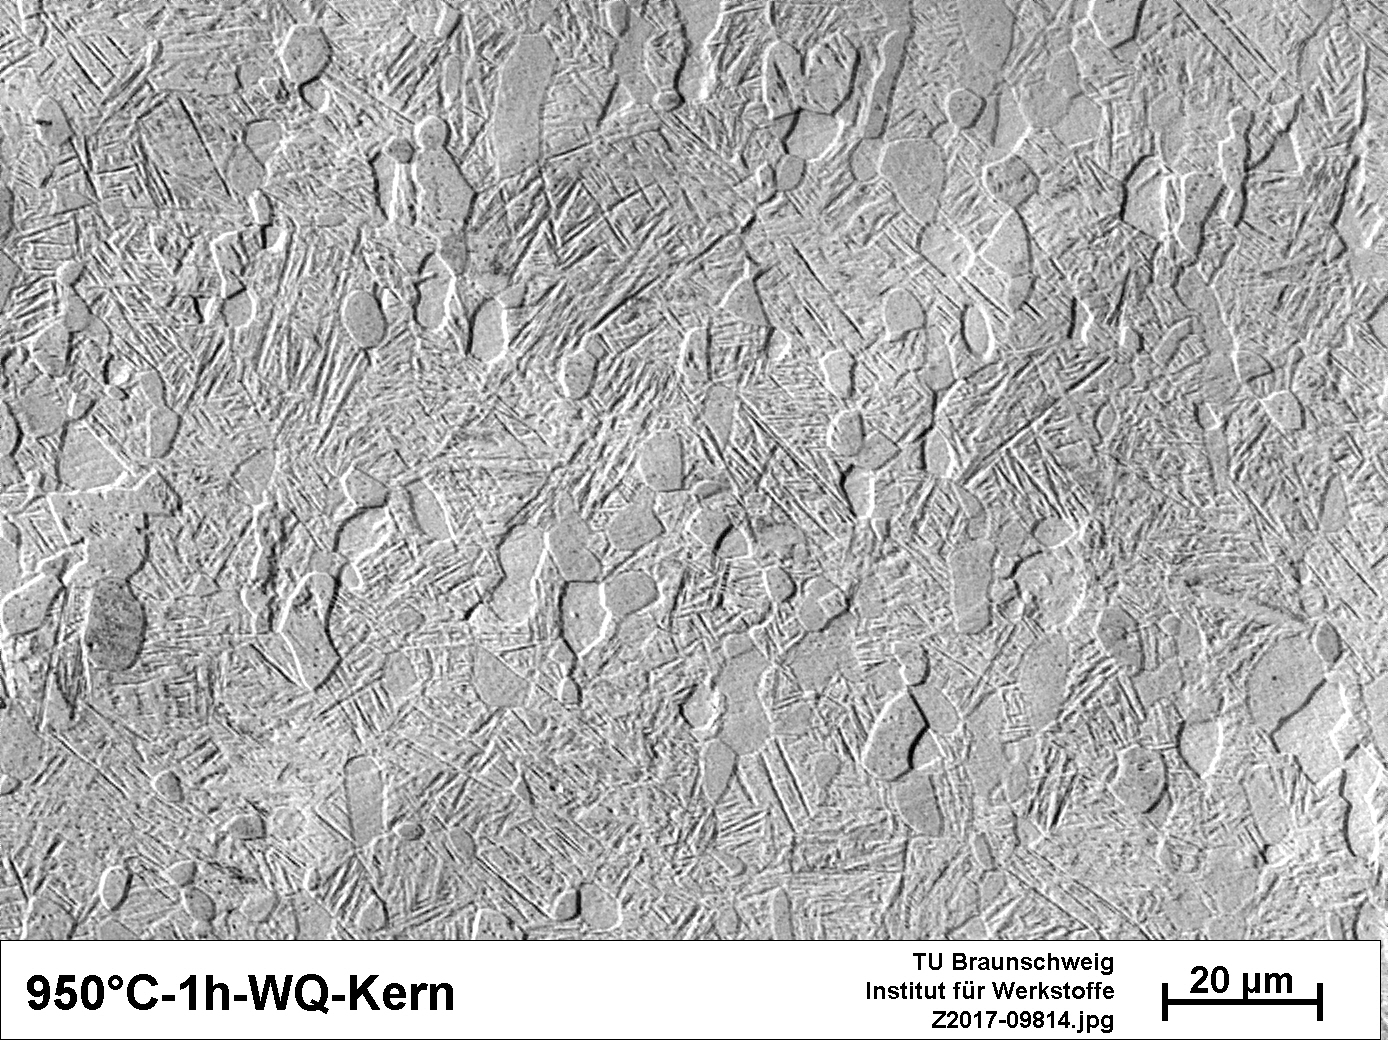
\includegraphics[width=0.49\textwidth]{Bilder/9501hwq.jpg}} 
	\caption{Gefüge ohne Auslagern}
	\label{Gefüge ohne Alterung}
\end{figure}
\begin{figure} 		%970°C und alterung
	\subfigure[Gefüge bei einer Glühungstemperatur von 970°C mit Auslagerung bei 520°C für 2h]{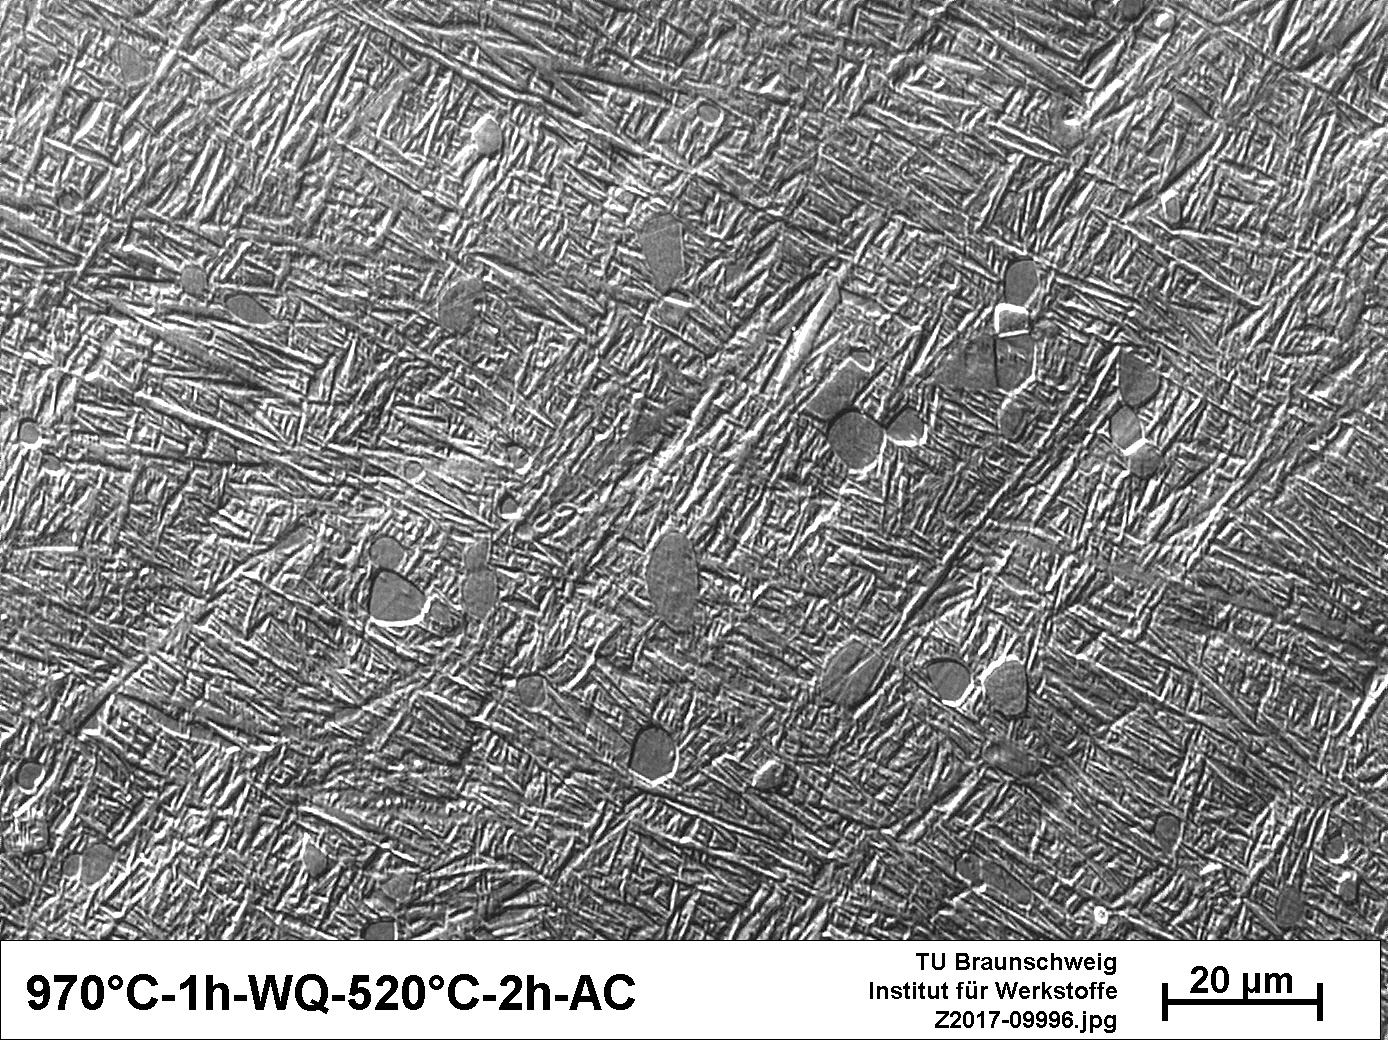
\includegraphics[width=0.49\textwidth]{Bilder/9701hwq5202hac.jpg}} 
    \subfigure[Gefüge bei einer Glühungstemperatur von 970°C mit Auslagerung bei 520°C für 8h]{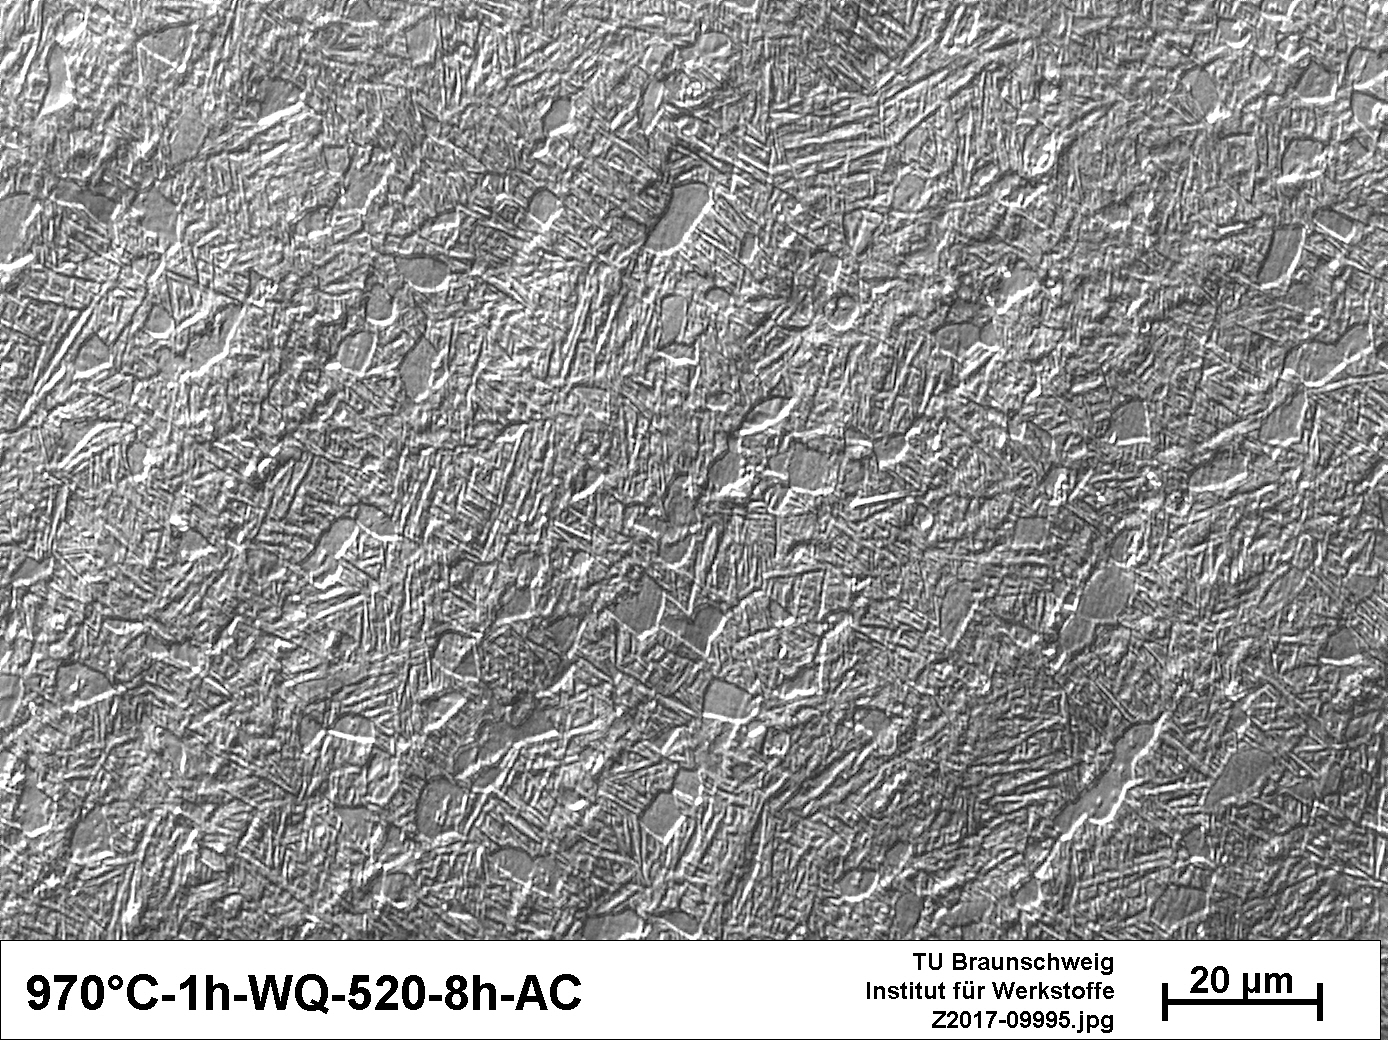
\includegraphics[width=0.49\textwidth]{Bilder/9701hwq5208hac.jpg}} 
    \caption{Gefüge mit einer Glühtemperatur von 970°C und unterschiedlichen Alterungszeiten}
    \label{970 alterung}
\end{figure}



\subsection{2. Wärmebehandlung: Verlängerte Haltezeit der Auslagerung}
Aus den Ergebnissen der ersten Wärmebehandlung lässt sich schließen, dass eine längere Haltezeit, innerhalb einer Auslagerung ausgehend von einer Glühtemperatur von 970°C, keine Festigkeitssteigerung hervorruft. Die Alterung der Probe mit einer Glühtemperatur von 950°C zeigt bereits eine Härtesteigerung von circa 3\%. Eine Zunahme der Härte bei längerer Haltezeit ist somit für die Proben mit einer Glühtemperatur von 970°C unwahrscheinlich. 

Da die kurzen Haltezeiten nur geringe Auswirkungen auf die Härte haben, werden längere Haltezeiten durchgeführt. Der Zerfall des Martensits kann so weiter fortschreiten, da während den verwendeten Haltezeiten die Diffusionsvorgänge möglicherweise nicht abgeschlossen werden konnten. Um zu prüfen, ob eine noch längere Haltezeit eine größere Härte steigernde Wirkung hervorruft, werden die Haltezeiten auf 16 und 24 Stunden angepasst. So lässt sich zeigen, ob der Zerfall des Martensits noch positiv hinsichtlich der Festigkeit statt finden kann. 



\begin{figure} %950°C und alterung
	\subfigure[Gefüge bei einer Glühungstemperatur von 950°C mit Auslagerung bei 520°C für 2h]		{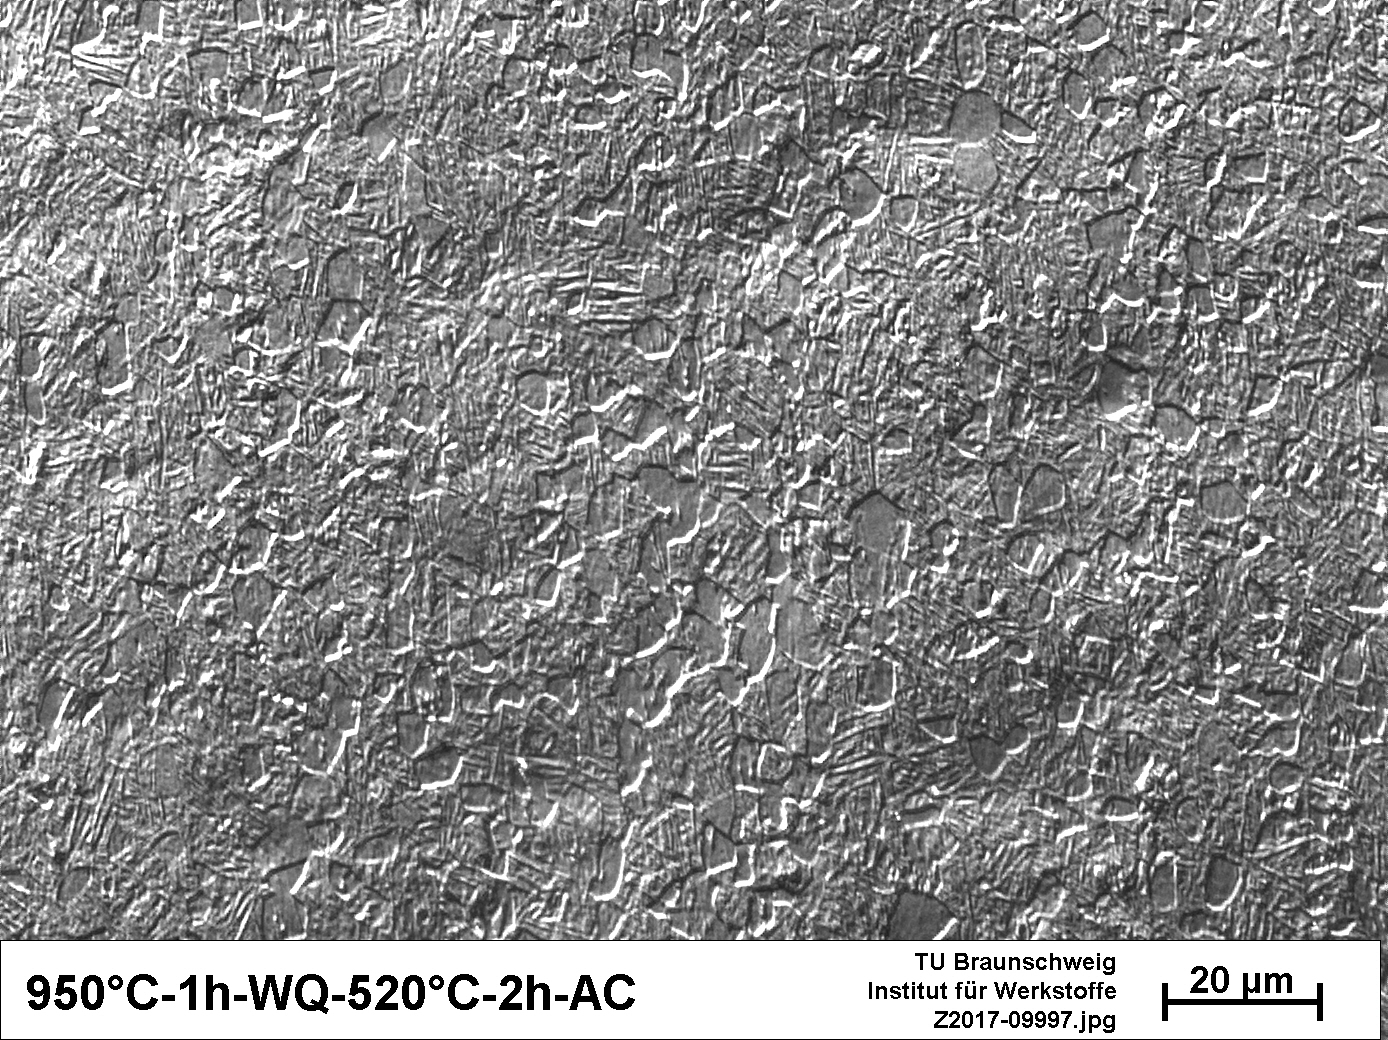
\includegraphics[width=0.49\textwidth]{Bilder/9501hwq5202hac.jpg}} 
    \subfigure[Gefüge bei einer Glühungstemperatur von 950°C mit Auslagerung bei 520°C für 8h]{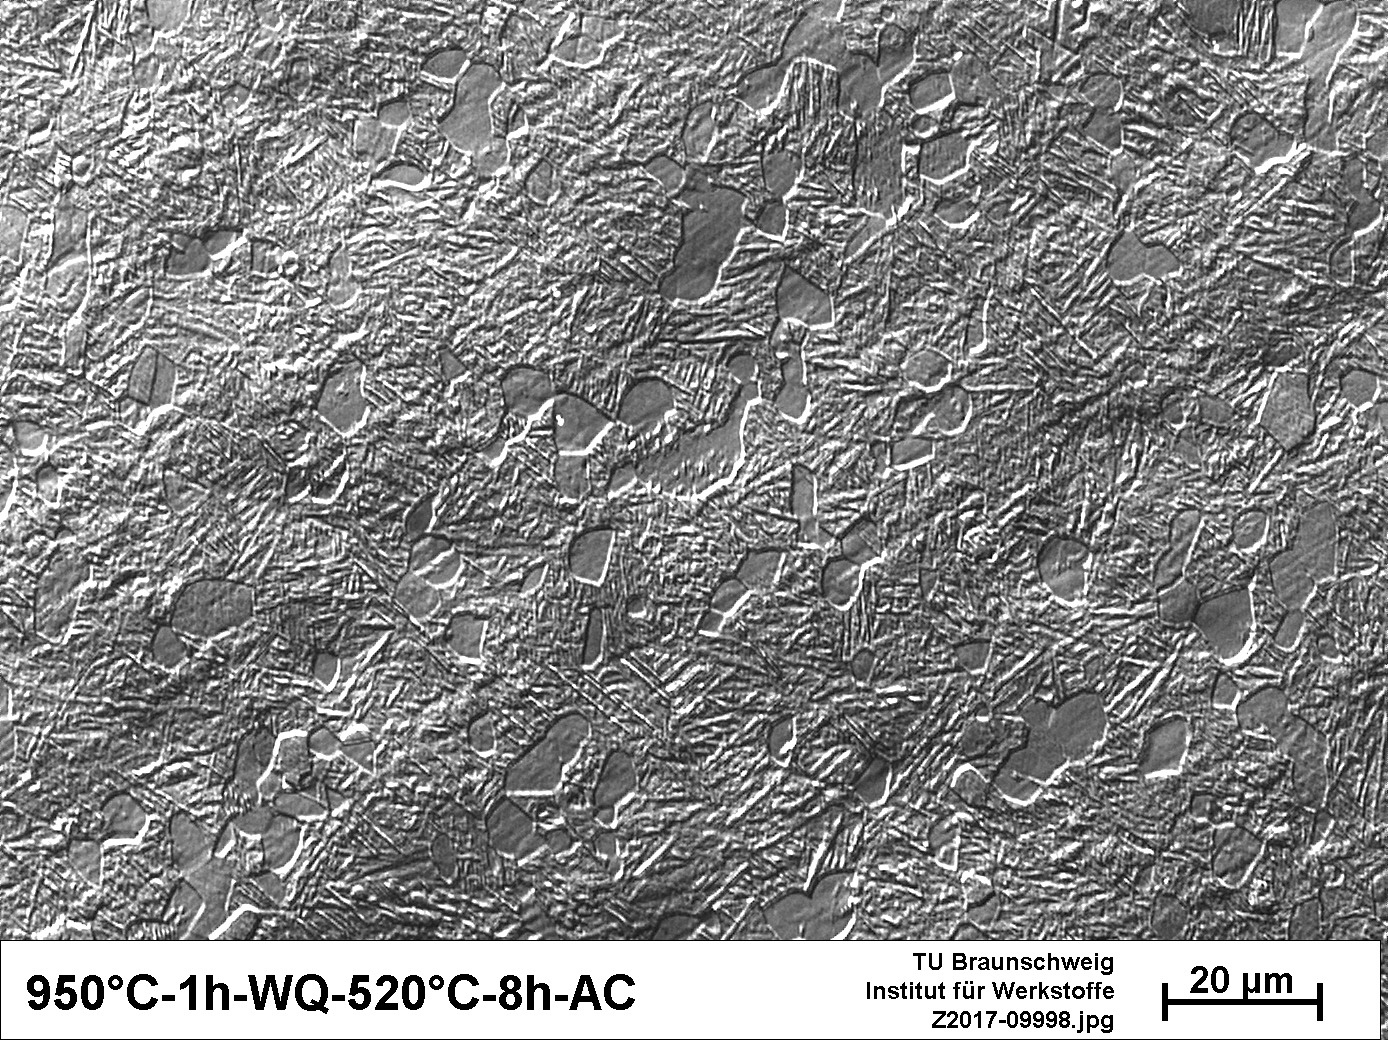
\includegraphics[width=0.49\textwidth]{Bilder/9501hwq5208hac.jpg}} 
    \caption{Gefüge mit einer Glühtemperatur von 950°C und unterschiedlichen Alterungszeiten}
    \label{Glühung950+alterung}
\end{figure}
\subsection{Ergebnisse mit längerer Haltezeit}
Die Härtewerte zeigen, dass aus einer längeren Haltezeit eine höhere Härte resultiert. Im Vergleich zu der Haltezeit von zwei Stunden zeigen die Ergebnisse aus Tabelle \ref{950 16 24} für eine Haltezeit von 16 und 24 Stunden eine nochmalige Härtesteigerung von 10 HV10. Die Härte nimmt also für längere Haltezeiten stetig zu. 

Aus den Gefügebildern mit dem Lichtmikroskop aus Abbildung \ref{950 lange auslagerung} ist keine qualitative Aussage über Veränderungen des Gefüges zu treffen. Dazu muss wie zuvor ein REM herangezogen werden.

Die Aufnahme aus Abbildung \ref{REM 950C 24h} zeigt eine REM-Aufnahme von dem 24 Stunden lang gealterten Gefüge. Das Martensit ist fast nicht mehr zu erkennen. Die ehemaligen Nadeln sind an vielen Stellen unterbrochen und als solche nicht mehr zu erkennen. Um das Alpha-Korn hat sich ein ausgeprägter Rand gebildet. Die für kürze Haltezeit beschriebene Vergröberung ist mit der Zeit noch einmal größer geworden.






\begin{figure}
\subfigure[Gefüge bei einer Glühungstemperatur von 950°C und 16 Stunden Alterung]{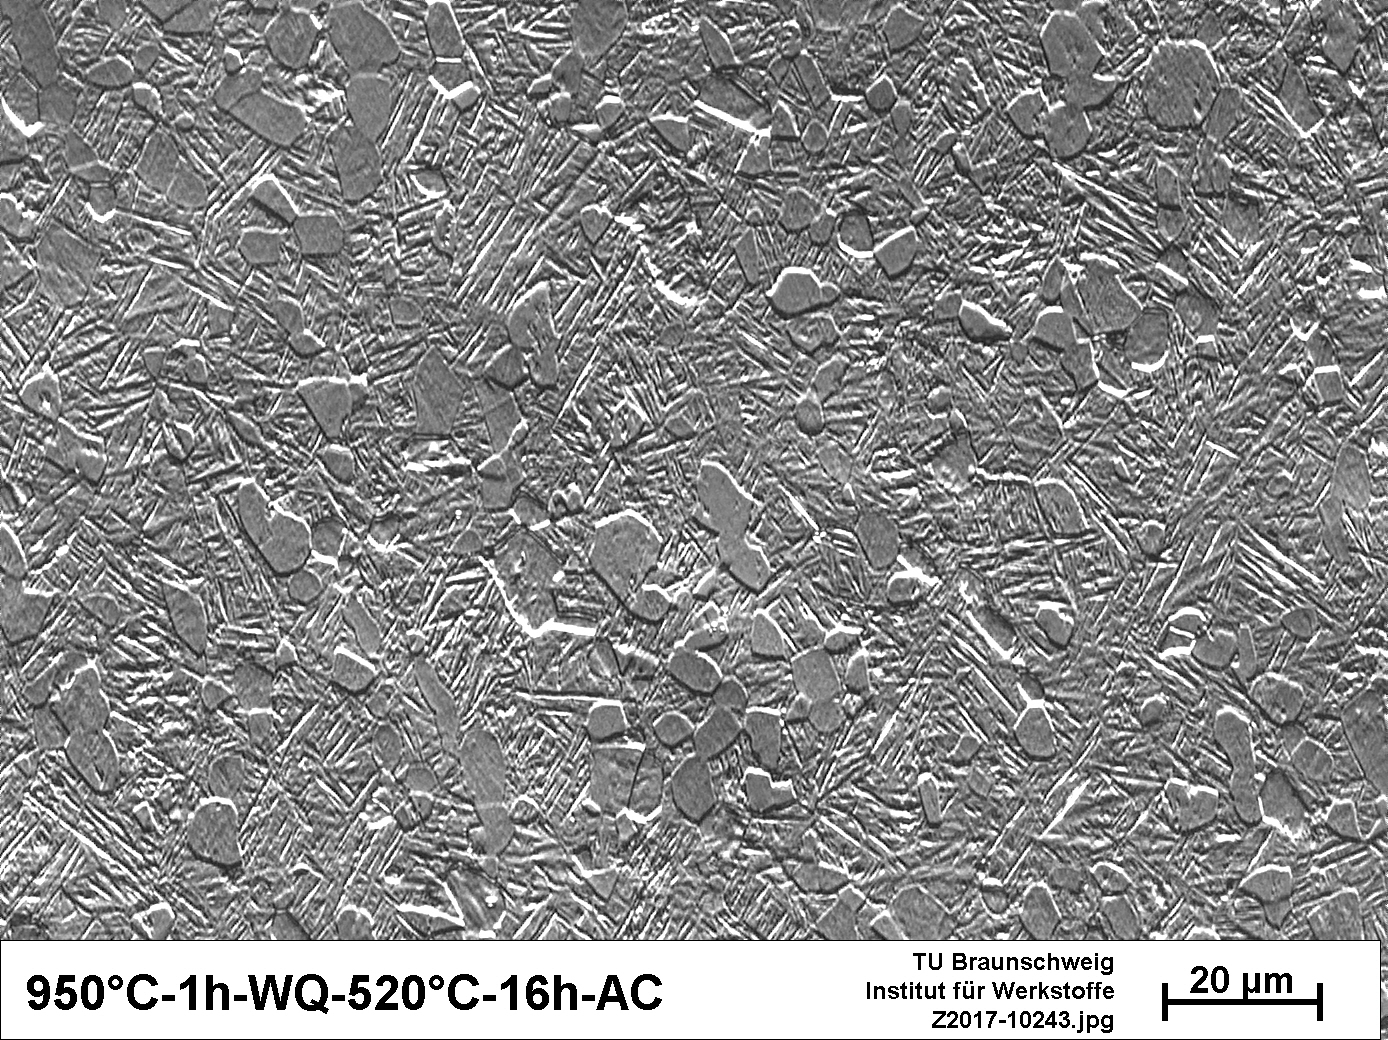
\includegraphics[width=0.49\textwidth]{Bilder/9501hwq52016hac.jpg}} 
    \subfigure[Gefüge bei einer Glühungstemperatur von 950°C und 24 Stunden Alterung]{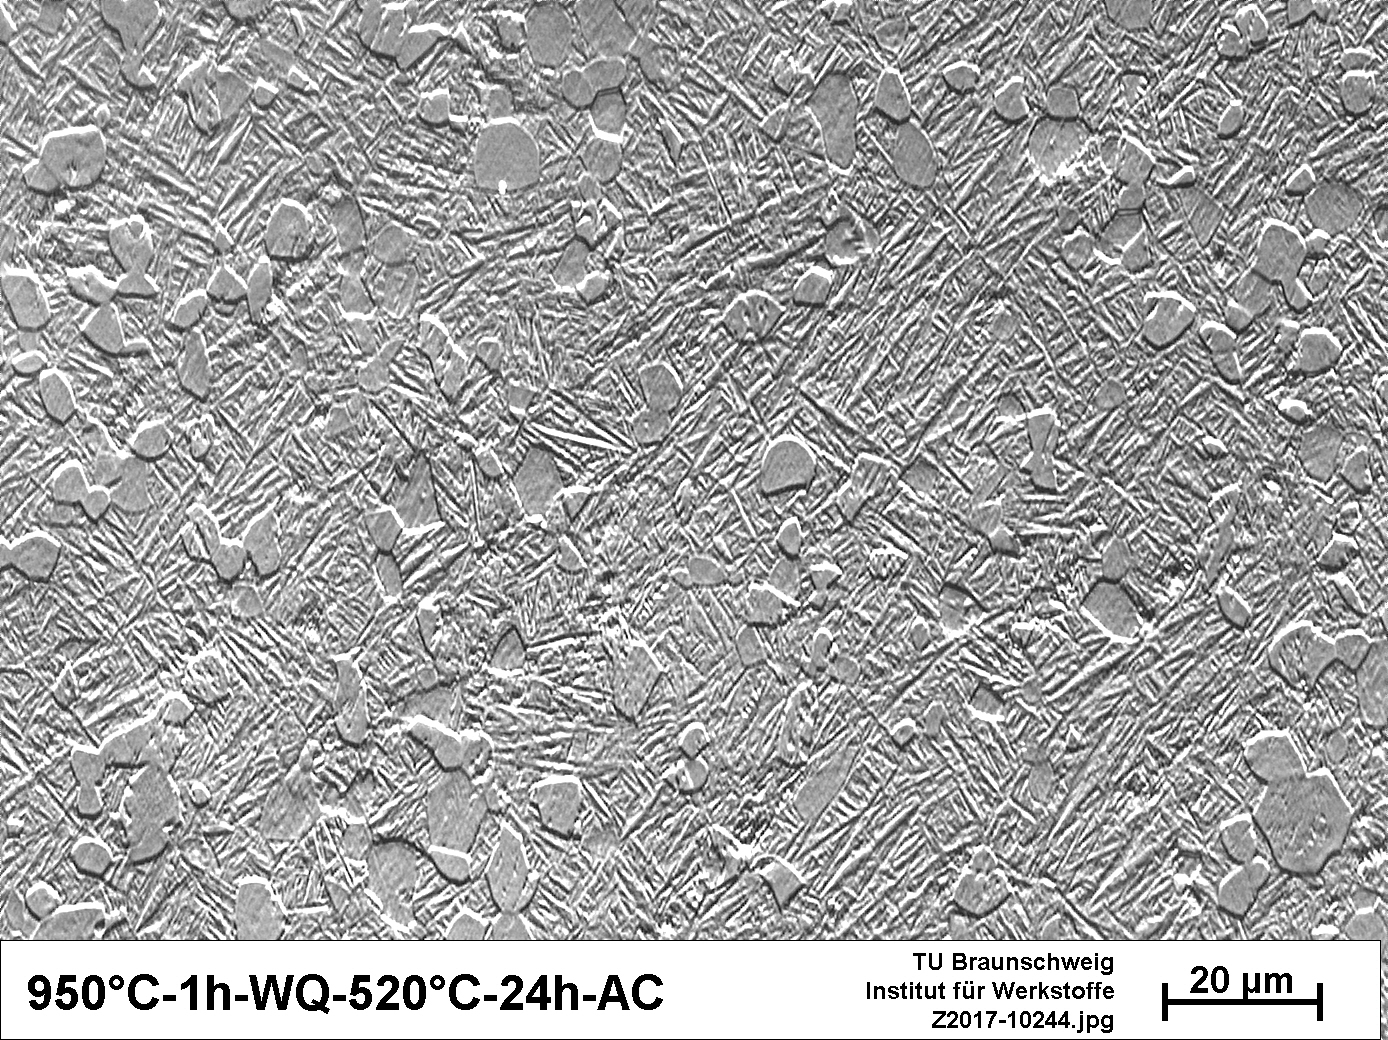
\includegraphics[width=0.49\textwidth]{Bilder/9501hwq52024hac.jpg}} 
	\caption{Gefüge bei 950°C bei 16h und 24h Auslagerung}
	\label{950 lange auslagerung}
\end{figure}

\begin{table}
\begin{tabular}{c|c}
\multicolumn{2}{c}{16h Auslagern} \\
\hline
Abstand in mm &	Härte in HV10 \\
0.02	&	359 \\
3.16	&	358 \\
6.31	&	362 \\
9.46	&	357 \\
12.60	&	360 \\
\hline
Mittelwert	&	359 \\
Max	&	362 \\
Min.	&	357 \\
Std.-abw.	&	1.79 \\
\end{tabular}
\begin{tabular}{c|c}
\multicolumn{2}{c}{24h Auslagern} \\
\hline
Abstand in mm	&	Härte in HV10 \\

0.02	&	362 \\
3.29	&	363 \\
6.55	&	363 \\
9.81	&	364 \\ 
13.07	&	363 \\
\hline
Mittelwert	&	363 \\
Max	&	364 \\
Min.	&	362 \\
Std.-abw.	&	0.803 \\
\end{tabular}
\caption{Härtewerte für eine Haltezeiten von 16 und 24 Stunden}
\label{950 16 24}
\end{table}

\begin{figure}
\centering
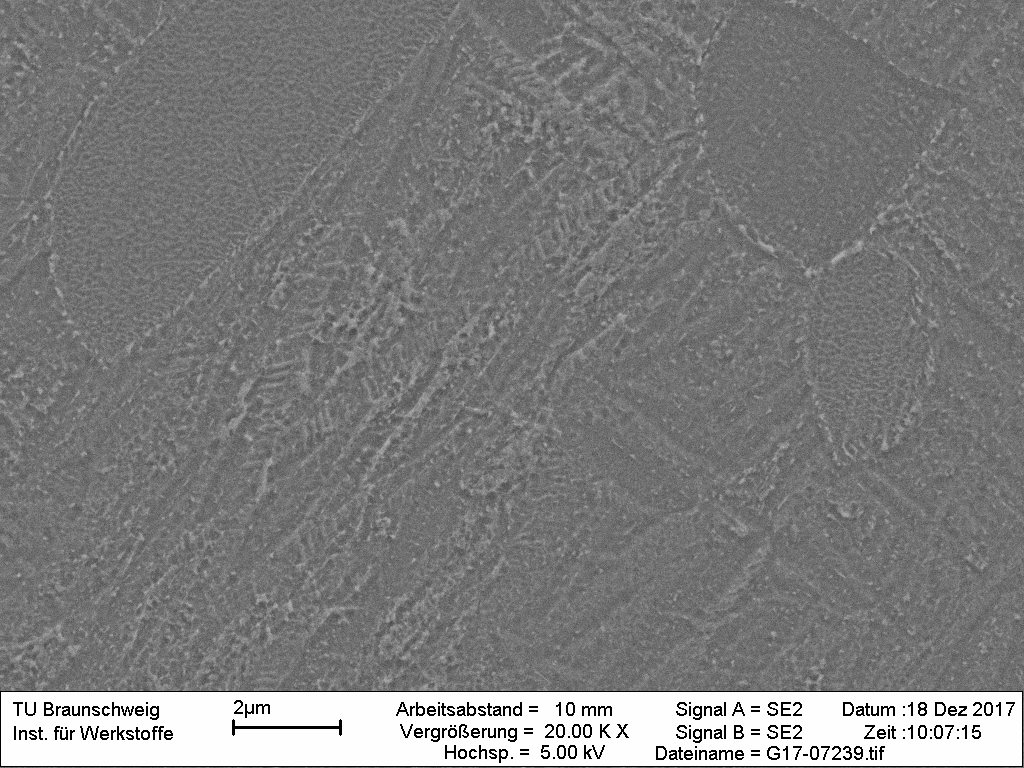
\includegraphics[width=0.66\textwidth]{Bilder/REM950C1hWQ520C24hAC.png}
\caption{REM Aufnahme: 950°C mit 24 Stunden Alterung}
\label{REM 950C 24h}
\end{figure}

\section{Ermittlung der Zugfestigkeit (Jannik Hansen)}\label{Kapitel ermittlung der Zugfestigkeit}

Für die Ermittlung der Zugfestigkeit wurden drei Gefügezustände ausgewählt. Die Zugversuche werden jeweils an zwei Proben durchgeführt und die gemittelte Zugfestigkeit des Gefüges zu bestimmen (siehe  \ref{Kapitel Zugversuch}). Ausgewählt wurden die Gefüge, mit der höchsten Härte. Das ist zum Einen das bei 970°C geglühte Primär Alpha-Martensit-Gefüge (Proben 4 und 5) und zum Anderen das für 24 Stunden gealtert,bei 950°C geglühte Primär Alpha-Martensit-Gefüge (Proben 6 und 7). Als drittes wurde ein vollmartensitisches Gefüge mit geringerer Härte geprüft (Proben 2 und 3). Zum Vergleich wird das Ausgangsgefüge gezogen (Probe 1).
\subsection*{Erwartungen}
Nach dem in Abschnitt \ref{Kapitel ti64} gegebenem Überblick dürften Werte für den Ausgangszustand zwischen 900 und 950 MPa erwartet werden. Die wärmebehandelten Proben sollten deutlich höher im Bereich von 1000 bis 1200 MPa liegen. Unter den wärmebehandelten Proben ist zu erwarten, dass die reinmartensitische Probe die mit der geringsten Festigkeit ist. Die bei 970°C geglühte Probe weist, von den einstufig geglühten Proben, den höchsten Härtewert auf. Höher war nur der Härtewert der bei 950°C geglühten, abgeschreckten und bei 520°C für 24 Stunden ausgelagerten Probe, bei der die höchste Zugfestigkeit zu erwarten ist.

\subsection*{Ergebnisse}

\begin{figure}
\centering
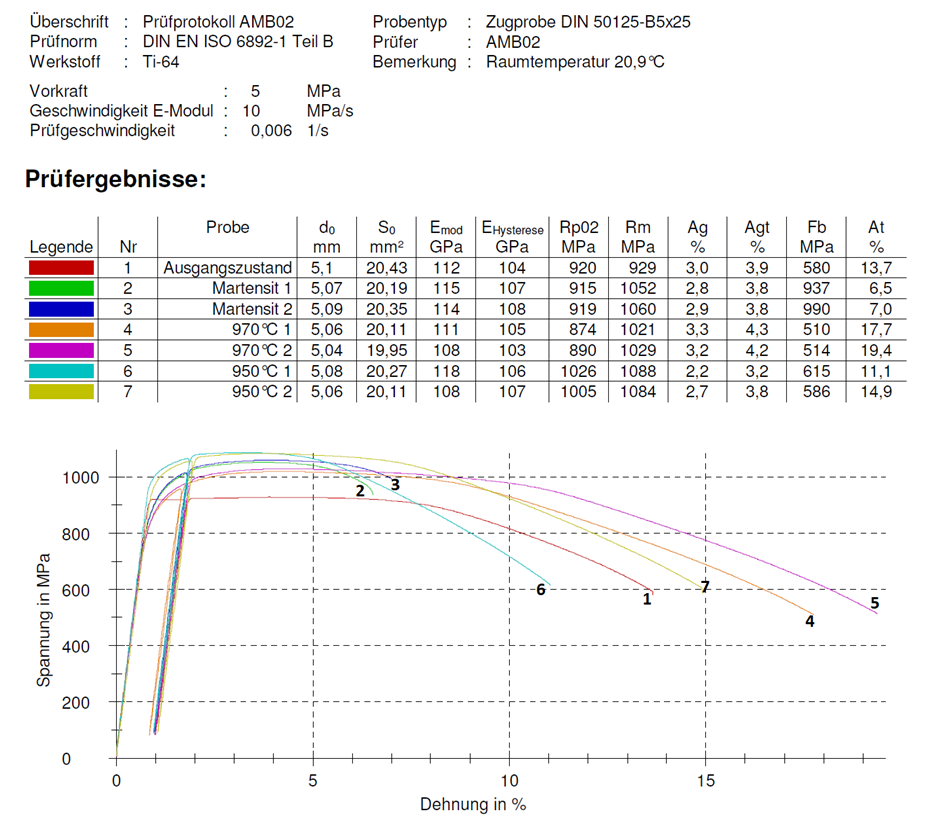
\includegraphics[angle=90, width=1\textwidth]{Bilder/haertepruefung.png}
\caption{Ergebnisse der Zugprüfungen}
\label{Ergebnisse der Zugpruefungen}
\end{figure}

Abbildung \ref{Ergebnisse der Zugpruefungen} zeigt im oberen Teil einen Ausschnitt aus dem Prüfprotokoll der durchgeführten Zugversuche. Darin sind die relevanten Werte E-Modul, Dehngrenze, Zugfestigkeit und Gesamtdehnung tabellarisch dargestellt. Die dort ermittelten Werte bestätigen die oben aufgestellten Vermutungen teilweise. Alle Proben haben eine höhere Zugfestigkeit als der Ausgangszustand. Die Proben 6 und 7 weisen die höchste Zugfestigkeit auf. Die rein martensitischen Proben 2 und 3 jedoch weisen eine höhere Zugfestigkeit als die Proben 4 und 5 auf. Der E-Modul liegt für alle Proben im Bereich von ungefähr 100 bis 115 GPa. Die Gleichmaßdehnung lag für alle Proben bei rund 3\%. Abbildung \ref{Ergebnisse der Zugpruefungen} zeigt im unteren Teil die während der Zugversuche aufgenommenen Spannungs-Dehnungskurven. Aus diesen lässt sich beispielsweise die Bruchdehnung ablesen. Für einen besseren Überblick wurden die Probennummern ergänzt.

Bei der Betrachtung des Graphen fällt zunächst die zweifache Bestimmung des E-Moduls mittels Hysterese Schleife auf.  Der Ausgangszustand erreicht eine Zugfestigkeit von 929MPa bei einer Bruchdehnung von rund 12,5\%. Das Ausgangsgefüge liegt somit im Bereich des oben bereits Erwarteten. Die voll-martensitischen Gefüge der Proben 2 und 3 erreichten gemittelt eine Zugfestigkeit von 1055MPa. Die Zugfestigkeit wurde durch das martensitische Gefüge also um 13,5\% gesteigert. Gleichzeitig sind diese Gefüge die sprödesten, sie erreichen eine Bruchdehnung zwischen 5,5\% und 6\%. Das spröde Werkstoffverhalten spiegelt sich an der Bruchfläche wieder. Diese Proben zeigten eine geringe Brucheinschnürung. Die Brucheinschnürung der anderen Proben war deutlicher ausgeprägt.

Die Proben 4 und 5 dagegen sind mit 16,5\% und 18,5\% Bruchdehnung am duktilsten. Die Bruchdehnung liegt damit sogar oberhalb des Ausgangszustandes. Sie erreichen mit gemittelten 1025MPa Zugfestigkeit eine Steigerung von nur 11\% gegenüber dem Ausgangszustand. Das ist auffällig, da das Primär Alpha-Martensit-Gefüge der Proben 4 und 5 eine höhere Härte aufweist, als das voll-martensitische Gefüge der Proben 2 und 3.

Die höchsten Zugfestigkeiten erreicht das ausgelagerte Primär Alpha-Martensit-Gefüge der Proben 6 und 7. Mit 1088MPa konnte die Zugfestigkeit gesteigert werden. Die Bruchdehnung streut hier mit 10,5\% und 14\% stärker als bei den anderen Proben, liegt im Mittel aber auf dem Niveau des Ausgangsgefüges. In Hinblick auf die Zugfestigkeit hat das ausgelagerte Primär Alpha-Martensit-Gefüge folglich mit knapp 17\% Steigerung gegenüber dem Ausgangszustand und gleichbleibender Duktilität am besten abgeschnitten. 

\chapter{Diskussion der erzielten Ergebnisse in Hinblick auf eine Gefügeoptimierung}
In diesem Kapitel werden die erzielten Ergebnisse näher erläutert. Es wird auf die Mechanismen die in den  einzelnen Wärmebehandlungen ablaufen eingegangen.

In jedem der Ansätze ging es um Festigkeitssteigerung durch eine erhöhte Grenzflächendichte. Diese wird durch ein feines Gefüge erzeugt. Die Versetzungen können bei einer großen Grenzflächendichte nur unter hohem Energieaufwand durch das Bauteil wandern. 
\section{Härtesteigerung durch das Primär-Alpha-Martensit-und Vollmartensit-Gefüge (Jannik Hansen)}\label{Kapitel einfluss des Primäralphaanteils}
Die in Kapitel \ref{Kapitel Abhängigkeit der Härte vom Primäralphaanteil} beschriebenen Ergebnisse der ersten Wärmebehandlung sollen nun diskutiert werden. Hierbei handelt es sich um ein Gefüge aus Primär Alpha und Martensit. Der Primär Alpha-Anteil sinkt mit steigender Glühtemperatur. Mit abnehmendem Primär Alpha-Anteil steigt die Härte.


Die Steigerung der Härte des Gefüges lässt sich zum einen auf die Bildung des Martensits zurückführen. Dennoch darf der Titan-Martensit nicht mit dem Stahl-Martensit gleichgesetzt werden. Da beim Titan-Martensit keine Zwangslösung eines Legierungselements auftritt, wie das beim Stahl mit Kohlenstoff der Fall ist, tritt keine nennenswerte Gitterverzerrung bei Titan auf. Damit verbunden sollte auch nur eine geringe Steigerung der Härte einhergehen. Die hier auftretende Erhöhung der Härte auf 343 HV10 (950°C-1h-WQ) ist dagegen signifikant höher als der Ausgangszustand mit 305 HV10. Es tritt also noch ein anderer Effekt auf.

Die erhöhte Grenzflächen, die aus dem feinen Martensit-Gefüge resultiert, erzeugt die Härtesteigeurng. Abbildung \ref{Vergleich Primäralpha martensit}(a) zeigt das Ausgangsgefüge, im Vergleich eingestellten Gefüge in (b). Die Martensit-Nadeln sind deutlich feiner verteilt als die Gefügebestandteile des Ausgangszustandes. Daraus resultiert eine höhere Anzahl von Grenzflächen zwischen Martensit-Nadeln.

\begin{figure}
\subfigure[Ausgangsgefüge]{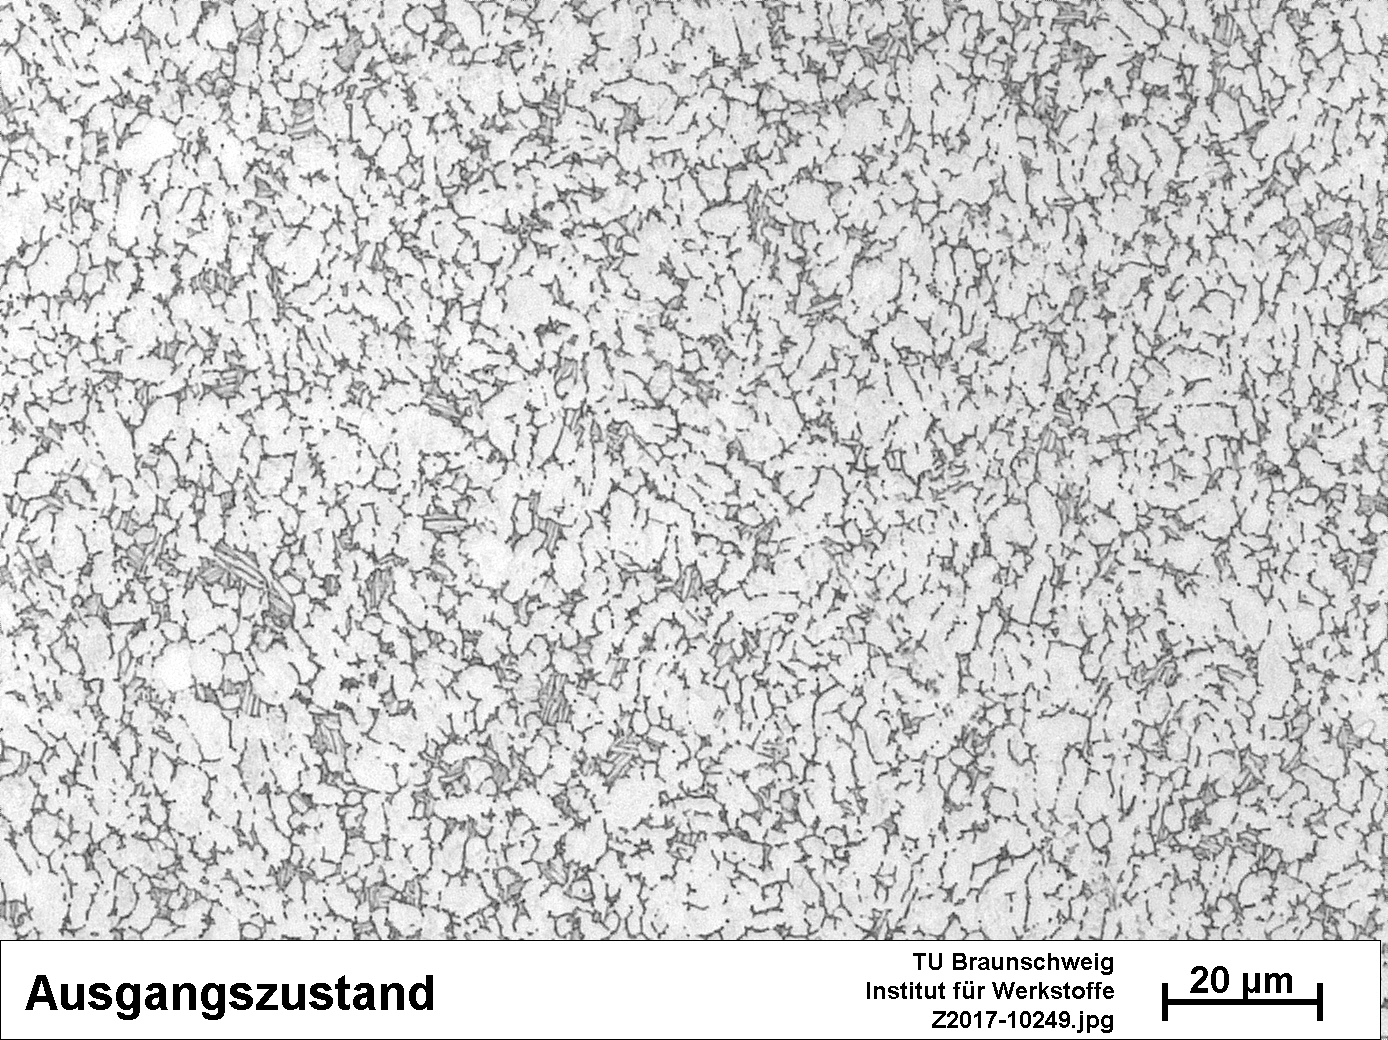
\includegraphics[width=0.5\textwidth]{Bilder/Ausgangsgefuege.jpg}}
\subfigure[Primäralpha + Martensit]{\includegraphics[width=0.5\textwidth]{Bilder/9501hwq.jpg}}
\caption{Vergleich zwischen Ausgangsgefüge und Primäralpha + Martensit}
\label{Vergleich Primäralpha martensit}
\end{figure}


Durch die erhöhte Grenzflächendichte werden die Versetzungsbewegungen am Voranschreiten gehindert. Eine erhöhte Spannung ist nötig damit die Versetzung durch das Gefüge wandert, was die Härte und Festigkeit steigert. Der größere Volumenanteil der Alpha-Körner (siehe Abbildung \ref{Vergleich Primäralpha martensit}(b)) wirkt sich negativ auf die Grenzflächendichte aus. Dies zeigt sich auch durch die Ergebnisse der Härteprüfung in Abschnitt \ref{Kapitel Abhängigkeit der Härte vom Primäralphaanteil}. 



\section*{Abnahme der Zugfestigkeit des Vollmartensit-Gefüges gegenüber dem Primär-Alpha-Martensit-Gefüge}
In Kapitel \ref{Kapitel Abhängigkeit der Härte vom Primäralphaanteil} wurde festgestellt, dass die ermittelte Härte mit sinkendem Primär Alpha-Anteil steigt. In Kapitel \ref{Kapitel einfluss des Primäralphaanteils} wurde die Härtesteigerung auf eine erhöhte Grenzflächendichte zurückgeführt. Demnach sind die in der Martensit-Matrix fein verteilten Martensit-Nadeln für die höhere Härte verantwortlich.
Es sollte somit ein vollmartensitisches Gefüge höhere Härtewerte besitzen.
Die Ergebnisse der Härteprüfung für ein vollmartensitisches Gefüge  widerlegen diese Aussage (siehe Kapitel \ref{Kapitel Bildung und Zerfall des Vollmartensits}). Die Härte ist im Verhältnis zum Gefüge mit einem geringen Alpha-Anteil gesunken. Gleichzeitig liegt die Härte auf dem Niveau der bei 950°C geglühten und wasserabgeschreckten Probe. Einen Überblick gibt Tabelle \ref{Tabelle Mittelwerte Härte für verschiedene Proben}.
\begin{table}
\begin{tabular}{c|c|c|c|c}
Probe & 950°C-WQ & 970°C-WQ & 1050°C-10min-WQ & 1050°C-30min-WQ \\
\hline
Härte[HV10] & 343 & 357 & 346 & 342 \\
\hline
Standardabweichung & 6,68 & 8,95 & 1,94 & 4,5 \\

\end{tabular}
\caption{Mittelwerte der Härte für verschiedene Proben}
\label{Tabelle Mittelwerte Härte für verschiedene Proben}
\end{table}

Die Martensit-Nadeln im vollmartensitischen Gefüge sind länger als die in dem Gefüge mit einem Rest an Alpha-Anteilen. Ein Vergleich der beiden Gefüge aus Abbildung \ref{Vollmartensit neben 960} macht dies ersichtlich. Die verbliebenen Alpha-Körner scheinen folglich das Wachstum der Martensit-Nadeln zu behindern. Der Anstieg der Härte wird also wie bereit in Kapitel \ref{Kapitel einfluss des Primäralphaanteils} gezeigt nicht nur von der Primär-Alpha-Phase behindert, sondern auch von zu großen Martensit-Nadeln. Zustände mit größter Härte würden also aus einem Gefüge mit einem geringen Alpha-Anteil entstehen. Die Probe mit einer Glühtemperatur von 970°C und einem Primär-Alpha-Anteil von circa 6\% kommt diesem sehr nahe.



\begin{figure}
\subfigure[Vollmartensit]{\includegraphics[width=0.5\textwidth]{Bilder/Vollmartensit.jpg}}
\subfigure[Abschrecken von 960°C]{\includegraphics[width=0.5\textwidth]{Bilder/9601hwq.jpg}}
\caption{Vollmartensit neben Primäralpha + Martensit Gefüge}
\label{Vollmartensit neben 960}
\end{figure}
Abbildung \ref{Vollmartensit neben 960} zeigt links eine oberhalb der Betatransus Temperatur geglühte und abgeschreckte Probe. Im Vergleich zur rechten Abbildung ist die deutlich gröbere Martensit-Matrix zu erkennen. Für die Länge der Martensit-Nadeln ist die Dauer und Temperatur des Glühens ausschlaggebend. Die maximale Länge der Martensit-Nadeln wird durch die größe eines ehemaligen Beta-Korns limitiert. Beim glühen oberhalb der Betatransus Temperatur ergibt sich nun folgende Schwierigkeit: Einerseits wird eine Temperatur oberhalb von Beta-Transus und ausreichend Zeit benötigt, um das gesamte Gefüge in die Beta-Phase umzuwandeln. Andererseits dürfen Temperatur und Haltezeit nicht zu hoch gewählt werden um das Wachstum der Beta-Körner zu minimieren. Die Temperatur hat einen größeren Einfluss auf die Diffusionsvorgänge und damit das Wachstum der Beta-Körner. [Mk2] Daher ist eine genaue Kenntnis der Beta-Transus-Temperatur des vorliegenden Materials für das Einstellen möglichst kleiner Beta-Körner notwendig.
Im Verlauf dieser Arbeit konnte die genaue Beta-Transus-Temperatur des Materials nicht bestimmt werden, weshalb für die rein martensitischen Proben Beta-Transus mit 1000°C angenommen wurde. Ein Lösungsglühen bei 50°C oberhalb Beta-Transus sollte die vollständige Umwandlung der Alpha-Phase bewirken. Vermuten lässt sich, dass die tatsächliche Beta-Transus-Temperatur unterhalb von 1000°C liegt. Eine Wärmebehandlung bei geringerer Temperatur als 1050°C wäre folglich ausreichend gewesen das Phasengemisch in Beta-Phase umzuwandeln. Daraus hätten demnach feinere Martensit-Nadeln erzeugt werden können. 


\section{Zerfall des Vollmartensits (Jonas Veer)}\label{Kapitel Zerfall des Vollmartensits}

Ziel ist es durch die Martensit-Nadeln eine hohe Grenzflächendichte zu erzeugen und im zweiten Schritt diese Nadeln zu unterteilen, sodass der Martensit durch Körner aus Alpha- und Beta-Phase unterbrochen wird, was in Abbildung \ref{Gefuegestruktur zweier Martensit Auslageungen} zu sehen ist. Die Körner stören die Versetzungsbewegung durch das Gefüge indem sie zusätzliche Grenzflächen bilden.

Der erste Wärmebehandlungsschritt bei 1050°C für 10 beziehungsweise 30 Minuten erzielten eine Verbesserung der Härte im Gegensatz zum Ausgangsgefüge.

Im zweiten Schritt der Wärmebehandlung wird der Martensit bei 800°C für zwei Stunden ausgelagert. Die Härte verbessert sich zwar im Vergleich zum Ausgangszustand (305 HV10) um 20 HV10, jedoch verliert es im Gegensatz zum unausgelagerten Martensit 20 HV10.

Der Zerfall ist in der Probe vollständig fortgeschritten und es lassen sich keine Martensit-Nadeln mehr erkennen. Das Ziel lediglich einen partiellen Zerfall des Martensits zu erzielen ist gescheitert. Durch einen partiellen Zerfall wären die Martensit-Nadeln durch Körner aus der Alpha und Beta Gleichgewichtsphase geteilt worden (siehe Abbildung \ref{Gefuegestruktur zweier Martensit Auslageungen}). Die Auslagerungstemperatur von 800°C war zu hoch oder die Haltezeit von zwei Stunden zu lang. 
Weitere Wärmebehandlung bei einer niedrigeren hätte einen unvollständigen Zerfall des Martensits zur Folge gehabt. Das Ziel der partiellen Unterbrechung der Platten durch Alpha- und Beta-Phase wäre steuerbar gewesen. 

Die Härtesteigerung im Vergleich zum Ausgangszustand kann auch hier durch eine hohe Grenzflächendichte in der Gleichgewichtsphase von Alpha und Beta erklärt werden. Die Beta-Körner sind längliche, feinverteilte Bereiche die sich in der Alpha-Phase.  
\section{Alterung des Martensits aus dem Primär-Alpha-Martensit-Gefüges (Tammo Stein)}
In der in Abschnitt \ref{Festigkeitssteigerung durch Martensitbildung} behandelten Wärmebehandlung ging es um den Zerfall des Martensits im Primär Alpha-Martensit-Gefüge. Dieser sollte in möglichst kleine Bereiche an Alpha- und Beta-Phase zerfallen. Nur so kann die Grenzflächendichte gegenüber dem Martensit erhöht werden. Der kritische Faktor war hierbei, inwiefern der Martensit zerfällt, während die Vergröberung als festigkeitsverringernder Prozess parallel abläuft. Ziel war es, diese konkurrierenden Prozesse so zu steuern, dass ein maximaler Festigkeitsgewinn entsteht. 

Ausgehend von den Ergebnissen der ersten Wärmebehandlung wurde festgestellt, dass ein niedriger Primäralpha-Anteil für eine Festigkeitssteigerung sorgt. Es würde also Sinn ergeben, das Gefüge mit dem geringsten Alpha-Anteil für die Alterung zu verwenden, um eine noch Höhere Härte zu erzielen. Wie bereits erwähnt entscheidet jedoch die Konzentration an Beta stabilisierenden Elementen in der Martensit-Phase ob ein festigkeitssteigernden Zerfall statt findet. In dem Gefüge mit wenig Primär-Alpha ist die Konzentration an Beta stabilisierenden Elementen auf Grund des großen Volummenanteils der Beta-Phase geringer als in Gefügen mit hohem Primär-Alpha-Anteil. Dies lässt darauf schließen, dass eine Auslagerung von Proben mit einer geringeren Glühtemperatur zu einer größeren Festigkeitssteigerung führt. Die Ergebnisse der Härteprüfungen zeigen genau den Fall. Proben mit einer Glühtemperatur von 970°C haben keine Festigkeitssteigerung erfahren, während die Proben mit einer Glühtemperatur von 950°C deutliche Festigkeitssteigerungen zeigen. So wird die am Anfang aufgestellte These bestätigt, dass für höhere Konzentrationen an Beta stabilisierenden Elementen eine Festigkeitssteigerung bei einer Alterung resultiert. 

Werden die Gefügebilder betrachtet, lässt sich das Ergebnis erklären. Bei der Auslagerung ausgehend einer Glühtemperatur von 970°C zeigt sich ein Zerfall des Martensits. Die ehemaligen Nadeln sind an vielen Stellen unterbrochen und es hat sich sekundäre Alpha- und Beta-Phase gebildet. Die entstandene Beta-Phase lässt sich den weißen Bereichen der REM Abbildungen zuordnen. Dieser Effekt ist bei der Haltezeit von acht Stunden noch stärker ausgebildet. Es ist allerdings auch zu beobachten, dass noch einige Nadeln unverändert vorliegen. Dies spricht für eine zu niedrige Haltezeit, da die Nadeln bei steigender Haltezeit eher zerfallen als bei einer kürzeren. Bei längeren Haltezeiten ist aber auch der konkurrierende Prozess stärker ausgeprägt. Bereits nach acht Stunden ist eine starke Vergröberung der Platten zu erkennen. Eine noch längere Haltezeit würde zu einem noch größeren Wachstum dieser Platten führen, sodass sich die Grenzflächendichte verringert und so die Festigkeit abnimmt. Eine Festigkeitssteigerung durch den Zerfall des verbleibenden Martensits ist also unwahrscheinlich, da die Vergröberung als Nebenprozess vorliegt. So ist auch die nicht vorhandene Festigkeitssteigerung zu erklären. Der Zerfall des Martensits liegt zwar vor und führt zu einer größeren Grenzflächendichte. Aber gleichzeitig resultiert durch die Vergröberung eine Abnahme der Grenzflächendichte. Es lässt sich also schließen, dass die beiden Prozesse aufgrund der konstanten Härtewerte in gleichen Maßen aufgetreten sind. 

Bei der Auslagerung ausgehend von einer Glühtemperatur von 950°C zeigt sich ein anderes Ergebnis. Die Härteprüfungen zeigen, dass aufgrund der Auslagerung eine Härtesteigerung von circa 10 HV10 resultiert ist. Bei einer Analyse der Gefügebilder dieser Proben werden die Unterschiede gegenüber den Proben mit einer Glühtemperatur von 970°C sichtbar. Bei einem Vergleich der Gefügebilder bei gleicher Haltezeit fällt auf, das die Nadeln bei der niedrigeren Glühtemperatur einen höheren Teilungsgrad besitzen. Außerdem sind die Nadeln nicht so grob geworden, wie die der hohen Temperatur. Die Aufteilung der Nadeln in kleine Bereiche erklärt die Festigkeitssteigerung der ausgelagerten Proben. Die Grenzflächendichte wird dadurch stark erhöht und so ist eine Ausbreitung der Versetzungen nur mit einem großen Energieaufwand möglich. 

Allerdings ist auch bei der niedrigeren Temperatur das Martensit-Gefüge noch deutlich zu erkennen. Bei einer Haltezeit von 24 Stunden ist der Martensit jedoch in großen Anteilen zerfallen. Die entstandene Beta-Phase ist in den Gefügebildern als helle Bereiche zu erkennen. Vermutlich wird sich auch sekundäre Alpha-Phase gebildet haben. Diese sind in der REM Aufnahme jedoch nicht zu erkennen. Die Martensit-Nadeln haben sich also so geteilt, dass die entstandenen Phasen immer abwechselnd vorliegen. So entsteht im Verhältnis zum nicht ausgelagerten Gefüge ein Gefüge mit mehr Grenzflächen, was zu der Festigkeitszunahme führt.

Der Martensit ist wegen der metastabilität der Phase zerfallen. Je mehr Beta stabilisierende Elemente der Martensit enthält, desto eher zerfällt dieser in Alpha- und Beta-Phase. Dadurch ist auch der Zerfall bei einer Probe mit geringerem Martensit-Anteil stärker ausgeprägt als der der hohen Temperaturen. Der konkurrierende Prozess tritt bei jeder Alterung auf. Die Vergröberung hatte jedoch geringeren Einfluss auf die Probe mit weniger Martensit-Phase, da die Martensit-Nadeln vorher zerfallenden sind. 


Die Ergebnisse des Zugversuchs zeigen gute mechanische Eigenschaften. Die Steigerung der Festigkeit wurde bereits erläutert. Die hohe Bruchdehnung ergibt sich aus der Duktilität der Probe. Diese ist aufgrund des Zerfalls des Martensits entstanden. Aus langen Nadeln haben sich kleine Bereiche an Alpha- und Beta-Phase gebildet. Die sind deutlich duktiler als die vorher vorhandene Martensit-Phase.


\section{Erkenntnisse aus dem Zugversuch (Jannik Hansen)}
\subsection{Schlussfolgerungen aus den im Zugversuch ermittelten Daten}
 Die Aufgabestellung stellt das Optimieren der Zugfestigkeit der Titanlegierung Ti 6Al 4V in den Fokus. Die Ergebnisse des Zugversuches haben gezeigt, dass mit dem ausgelagerten Primär Alpha-Martensit-Gefüge die höchste Zugfestigkeitssteigerung erzielt wird. Nicht nur wurde die Zugfestigkeit um knapp 160MPa gesteigert, sondern auch die Duktilität auf ähnlichem Niveau wie die des Ausgangsgefüges gehalten. Dennoch streuten die Bruchdehnungen dieses Gefüges am stärksten. Um allerdings bessere Aussagen treffen zu können sollte ein größerer Probenumfang gewählt werden.
\subsection{Diskussion der Korrelation zwischen Härte und Zugfestigkeit}
Die Ergebnisse aus Abschnitt \ref{Kapitel ermittlung der Zugfestigkeit} zeigen, dass die Zugfestigkeit mit der Härte steigt. Einzige Ausnahme bildeten die bei 970°C geglühten Proben. Hier wurde im Vergleich zu den bei 950°C geglühten und ausgelagerten Proben eine um 60 MPa geringer Zugfestigkeit gemessen. Die zuvor ermittelte Härte lag bei beiden Proben jedoch bei rund 360 HV10. Offensichtlich müssen die durch das Auslagern erfolgte Gefüge Änderung hier einer Rolle spielen. Eine Genaue Schlussfolgerungen auf die Zugfestigkeit durch ermittelte Härtewerte.
In Abschnitt \ref{Kapitel Härte} wird auf eine mögliche Korrelation zwischen dem für eine Probe ermittelten Härtewerten und der Zugfestigkeit geschlossen. Im Zuge dessen wurden zwei Möglichkeiten für eine Abschätzung aufgeführt. Im Folgenden sollen die Ergebnisse der Abschätzungen nach Zwicker [19] (Variante1) und der Autoren von Quelle [9] (Variante2) mit der tatsächlichen Zugfestigkeit verglichen werden. 
Die Ergebnisse der Abschätzungen werden in Tabelle \ref{Tabelle Zugfestigkeits härte korrelation} aufgeführt.
\begin{table}
\begin{tabular}{c|c|c|c|c|c}
Probe & Härte  & Variante 1  & Variante 1  & Variante 2 & Zugversuch  \\
& [HV10] & min. [MPa] & max. [MPa] & [MPa] & [MPa]\\
\hline
Ausgangszustand & 305 & 927 & 1047 & 856 & 929 \\
\hline
Martensit & 346 & 1052 & 1188 & 1003 & 1055 \\
\hline
970°C & 357 & 1085 & 1225 & 1042 & 1025 \\
\hline
950°C & 363 & 1103 & 1246& 1064 & 1085 \\
\end{tabular}
\caption{Ergebnisse der Zugfestgkeits-Härte-Korrelation}
\label{Tabelle Zugfestigkeits härte korrelation}
\end{table}
Die Ergebnisse zeigen, dass eine Abschätzung nach der von Zwicker vorgeschlagenen Methode mit einem Faktor von 0,31 annähernd die genaueste Abschätzung liefert. Nach der Variante der Messwert für die bei 970°C geglühte Probe einen Ausreißer darstellt. Die Korrelation zwischen Zugfestigkeit und Härtewert scheint dennoch nicht sonderlich gut. Ausschlaggebend hierfür ist, dass für die martensitischen Proben zwar geringere Härtewerte ermittelt wurde, deren Zugfestigkeit im Versuch jedoch oberhalb von der bei 970°C geglühten Proben liegen. Ein Funktionaler Zusammenhang kann so demnach nicht durch die oben behandelten linearen Zusammenhänge beschrieben werden. Der von Matthew J.D. Jr. in \cite{Donachie2001} getroffenen Aussage (siehe \ref{Kapitel Härte}) lässt sich folglich zustimmen. Für Titanwerkstoffe scheint es zumindest auf Basis der hier zugrundeliegenden Ergebnisse keine gute Korrelation zwischen Zugfestigkeit und Härte zu geben.
\chapter{Ausblick (Jonas Veer)}
Die Aufgabenstellung verlangt die Gefügeoptimierung einer Fanschaufel aus der Titanlegierung Ti 6Al 4V hinsichtlich der Maximierung der Zugfestigkeit. Dazu sollen drei Wärmebehandlungen durchgeführt werden. Hinsichtlich der Zugfestigkeit ist das Gefüge der Wärmebehandlung 950°C-1h-520°C-24h am besten.
Jedoch ist für die Auslegung einer Fanschaufel nicht nur die Zugfestigkeit als alleiniger Parameter zu berücksichtigen. Weitere Eigenschaften, die für die Wahl des optimalen Gefüges entscheidend sind, sind Bruchdehnung und Dauerfestigkeit.

Die Bruchdehnung ist mit 10,5\%-14,0\% sehr gut und liegt im Bereich des Ausgangsgefüges (12,5\%). 
Die Dauerfestigkeit lässt sich durch einen Dauerschwingversuch ermitteln. Ein Wöhlerversuch ist sehr zeitintensiv und bedarf besonders für Titanlegierungen eines hohen Zeitaufwands. Da Titan eine schlechte Wärmeleitfähigkeit besitzt muss ein solcher Versuch bei einer niedrigen Frequenz durchgeführt werden um eine Erwärmung des Kerns der Probe zu vermeiden. Um von einer dauerfesten Probe auszugehen muss ein Lastenwechsel von 107 erreicht werden.
Die Dauerfestigkeit kann jedoch auch von der Zugfestigkeit abgeschätzt werden. Es kann von Dauerfestigkeiten in der Größenordnung von 40\% bis 50\% der Zugfestigkeit für Titanlegierungen ausgegangen werden \cite{Luetjering2007}.

Im Verlauf des Projekts kam es schon früh zu einer einseitigen Festlegung auf die Strategie, die beinhaltet verschiedene Martensitanteile im Gefüge einzustellen und daraufhin den Martensit zerfallen zu lassen. Dadurch erfolgte ein Ausschluss anderer Wärmebehandlungen. Eine Diversifizierung und damit eine variantenreichere Auswahl an Gefügen wäre möglich gewesen (siehe Kapitel \ref{Abschnitt Gefügemerkmale}). 
Ein weiterer Zerfall des Vollmartensits bei unterschiedlichen Temperaturen hätte die Schlussfolgerung (Kapitel \ref{Kapitel Zerfall des Vollmartensits}) untermauert. Dies wäre ein sinnvoller Schritt gewesen, da die Quellen von einer Härte von bis zu 410 HV10 ausgingen und somit eine hohe Festigkeit in den Zugversuchen zu erwarten war. Eine Versuchsreihe mit Auslagerungstemperaturen von 600°C- 800°C mit Schritten von 50°C wäre durchzuführen.

Die Erfolgreichen Zugversuche zeigten, dass eine Spezialisierung auf eine Gefügeeinstellung aus verschiedenen Martensitbehandlungen sich nicht als nachteilig herausstellte. 

\bibliographystyle{plain}
\bibliography{literatur}
\listoffigures
\listoftables
\end{document}
